% !BIB program = biber
\documentclass[11 pt]{article}

\usepackage{verbatim}
\usepackage[a4paper,margin=1in]{geometry}
\usepackage{booktabs}
\usepackage{adjustbox}
\usepackage{kotex}
\usepackage{threeparttable}
\usepackage[normalem]{ulem}

\usepackage{tikz}
\usetikzlibrary{positioning,arrows.meta,calc}

\usepackage{afterpage} % To avoid any unnecessary page breaks
\usepackage{pdflscape} % To use rotated pages
\usepackage{rotating}
\usepackage{float}

\usepackage{caption}
\captionsetup{width=0.8\textwidth}
\captionsetup[table]{skip=8pt}

\usepackage{subcaption}

\newcommand{\sym}[1]{\ensuremath{^{#1}}}
\newcommand{\bh}[1]{\textcolor{purple}{#1}}
\newcommand{\ms}[1]{\textcolor{olive}{#1}}
\newcommand{\es}[1]{\textcolor{orange}{#1}}

%%% --- 새 Section 3 / Appendix 를 위한 추가 ---
% 1. TikZ 그림에서 쓰는 색
\definecolor{groupc}{RGB}{20,20,20}
\definecolor{memj}{RGB}{31,78,121}
\definecolor{memi}{RGB}{176,48,48}
\definecolor{sand}{RGB}{228,216,192}

% 2. \autoref 이름 (없으면 "Lemma 1" 대신 "1"로 출력됨)
\providecommand{\definitionautorefname}{Definition}
\providecommand{\lemmaautorefname}{Lemma}
\providecommand{\propositionautorefname}{Proposition}
\providecommand{\remarkautorefname}{Remark}

%%%%%%%%%%%%%%%%%%%%%%%%%%%%%%%%%%%%%%%%%%%%%%%%%%%%%%%%%%%%%%%%%%%%%%%%%%%%%%%%%%%%%%%%

\input{style}
% Keep PDF destinations unique when appendix page numbering restarts.
\hypersetup{hypertexnames=false}

\addbibresource{bib.bib}

\newcommand{\RR}{\mathbb{R}}

\usetikzlibrary{arrows,positioning,calc}
\newcommand\LM{\ensuremath{\mathit{LM}}}
\newcommand\IS{\ensuremath{\mathit{IS}}}
\newcommand\bbar{\rule{0.5em}{0.15mm}}

%\usepackage{lscape} % To use landscape pages

\setlength{\tabcolsep}{7pt} % This line is to use wider columns in tables. Default value: 6pt
\renewcommand{\arraystretch}{1.2} % This line is to use larger rows in tables. Default value: 1

\def\tcr{\textcolor{red}}
\def\tcb{\textcolor{blue}}
\def\tcw{\textcolor{brown}}

\tikzset{
    %Define standard arrow tip
    >=stealth',
    %Define style for boxes
    punkt/.style={
           rectangle,
           rounded corners,
           draw=black, very thick,
           text width=6.5em,
           minimum height=2em,
           text centered},
    % Define arrow style
    pil/.style={
           <-,
           thick,
           shorten <=2pt,
           shorten >=2pt,},
    % Node for explanation       
    punk/.style={
           rectangle,
           draw=white, thin,
           text width=17em,
           minimum height=2em,
           text centered}   
}

\makeatother
\geometry{left= 1 in, right= 1 in, top= 1 in, bottom= 1 in}



\renewcommand{\subsectionautorefname}{Section}
\renewcommand{\sectionautorefname}{Section}
\renewcommand{\subsubsectionautorefname}{Section}

%%%%%%%%%%%%%%%%%%%%%%%%%%%%%%%%%%%%%%%%%%%%%%%%%%%%%%%%%%%%%%%%%%%%%%%%%%%%%%%%%%%%%%%%

\begin{document}

\title{Rationality-Based Preference Aggregation\thanks{We have benefited from conversations with Matthew Chao, Wonki Cho, Federico Echenique, and Sung-Ha Hwang. We also thank Youngjae Hwang, Jieun Hong, Wonsik Ko, Jahyeon Koo, Eunjae Lee, Jiyeong Lee, and Myungkou Shin for their excellent research assistance. This paper is financially supported by Korea Development Institute Research Grant and Mid-Career Bridging Program through Seoul National University. Author names are in alphabetical order.} \\}

\author{
\begin{tabular}[t]{c@{\hskip 5em}c@{\hskip 5em}c}
 Syngjoo Choi\footnote{Department of Economics, Seoul National University. \href{mailto:syngjooc@snu.ac.kr}{syngjooc@snu.ac.kr}} &
 Byunghun Hahn\footnote{Department of Economics, Seoul National University. \href{mailto:bhhahn@snu.ac.kr}{bhhahn@snu.ac.kr}} &
 Booyuel Kim\footnote{Graduate School of Environmental Studies, Seoul National University. \href{mailto:booyuel@snu.ac.kr}{booyuel@snu.ac.kr}} \\[0.5em]
 Minseon Park\footnote{Department of Economics, University of Michigan. \href{mailto:minseonp@umich.edu}{minseonp@umich.edu}} &
 Yoonsoo Park\footnote{Division of Economics, Sookmyung Women's University. \href{mailto:yoonpark@sm.ac.kr}{yoonpark@sm.ac.kr}} &
 Euncheol Shin\footnote{College of Business, Korea Advanced Institute of Science and Technology, \href{mailto:eshin.econ@kaist.ac.kr}{eshin.econ@kaist.ac.kr}} 
\end{tabular}
}


\date{
\today
}

\maketitle

\sloppy%avoids the breakage of words at the end of lines, by adjusting spaces between words inside the lines

\onehalfspacing

\begin{abstract}

We study how individual rationality shapes collective choice using a panel experiment with randomly assigned pairs. We develop a nonparametric revealed-preference distance that measures how closely collective choices align with each member’s individual choices without requiring rationalizable behavior or parametric utility assumptions. Collective choices are substantially closer to those of the more rational member, a pattern robust to placebo and disjoint-choice tests. Collective rationality, however, depends on both members: the CCEIs of the higher- and lower-CCEI members positively predict group CCEI, with the latter especially important. The results link individual rationality to preference aggregation and collective decision quality.


%We study how individual rationality affects group decision making using large-scale experiments with randomly assigned pairs. We develop a nonparametric revealed preference measure of bargaining power that applies to all subjects without requiring rationality or parametric utility functions. More rational individuals exert substantially greater influence on group decisions. Group decision quality increases with the rationality of the more rational member and decreases with the gap between members. The advantage of rational members is larger when communication is easier. Results establish causal effects of rationality on both bargaining power and collective choice quality.
%Many economic decisions are made by groups, yet models typically assume groups behave as single rational agents. We investigate how individual rationality shapes collective outcomes using large-scale experiments with 1,304 middle school students in South Korea randomly assigned into pairs to make repeated choices under risk. We introduce a novel nonparametric revealed-preference measure of bargaining power derived from the Critical Cost Efficiency Index (CCEI). Our measure quantifies how closely group choices align with each member's preferences without requiring parametric utility assumptions or restricting analysis to highly rational subjects. More rational individuals exert substantially greater influence: the revealed preference distance is 35-44 percentage points lower for the more rational member. Group decision quality increases with the most rational member's CCEI but decreases with the rationality gap between members. Individual rationality is the primary determinant of bargaining power, outweighing risk preferences, cognitive ability, friendship, and demographics. These findings establish causal effects of individual rationality on both the distribution of influence within groups and the quality of collective decisions.
\end{abstract}

\strut

\textbf{Keywords:} Revealed preference; Collective choice; Preference aggregation; Economic rationality; Group decision making; Experiment

\strut

%\pagebreak%breaks to the next page

\doublespacing %makes space between lines to be double, use singlespacing for space 1

%%%%%%%%%%%%%%%%%%%%%%%%%%%%%%%%%%%%%%%%%%%%%%%%%%%%%%%%%%%%%%%%%%%%%%%%%%%%%%%%%%%%%%%%

\section{Introduction}
\label{sec:introduction}
\input{intro_v2.tex}



%%%%%%%%%%%%%%%%%%%%%%%%%%%%%%%%%%%%%%%%%%%%%%%%%%%%%%%%%%%%%%%%%%%%%%%%%%%%%%%%%%%%%%%%%%%%%%%%%%%%%%%%%%%%%%

\section{Experiment and Data Collection}
\label{sec:data_collection}

We conducted large-scale lab-in-the-field experiments in 12 middle schools in Daegu, the fourth-largest city in South Korea, in coordination with the Daegu Metropolitan Office of Education. Data were collected in two waves, in August  and December 2016. Each wave consisted of two components: (i) individual and group decision-making experiments under risk and (ii) surveys measuring individual and social factors that may shape group decision-making. We administered the same experiment and survey modules in both waves. We rented laptops and set them up in participating classrooms. All sessions were computerized through oTree \citep{Chenetal:2015:JBEF} on these laptops connected to a classroom Wi-Fi router; \autoref{fig:photoshoot} in the Appendix shows a photograph from the fieldwork.

% TODO: Instructions PDF is present but not included; verify its version (20 choices versus 18 in the paper) before citing the appendix.
The experiment was conducted in four randomly selected classes per school, and the same four classrooms participated in both waves.\footnote{The number of seventh-grade classrooms ranged from six to nine across schools.} Four trained research assistants ran sessions concurrently across classrooms. To minimize differences in implementation across classes, we used standardized presentation slides and scripts, and the same research assistant visited the same classroom in both waves. See appendix XXX for slides and scripts distributed to experimenters. Any remaining differences across classrooms or experimenters are absorbed by class fixed effects included in the regression specifications.

In total, the decision-making experiment was completed by 1,572 students at baseline, 1,425 of whom also participated at endline. After excluding 121 students, our main analysis sample consists of 1,304 students in 652 pairs with valid matched-pair data in both waves.\footnote{The exclusions comprise 101 students whose partners changed across waves, four students in pairs with incomplete baseline choice records, six students in pairs with invalid collective choices, and ten students excluded for XXX.}


%%%%%%

\subsection{Experimental Design}
\label{subsec:design}

Our experimental design closely follows \citet{Choietal:2007:AER}. Each subject made a series of portfolio choices under risk. There were two equally likely states of nature, $s \in \{r, b\}$, and two corresponding Arrow securities. A choice is represented by $(x_r, x_b)$ on a normalized linear budget, $p_r x_r + p_b x_b = 1$, where $x_s \geq 0$ is the demand for the security paying in state $s$ and $p_s > 0$ is its price. Experimenters explained this choice environment using the red-blue urn analogy: one ball would be drawn from an urn containing equal numbers of red and blue balls, and each security would pay only if a ball of the corresponding color was drawn. \autoref{fig:decition_problem_example} illustrates the choice environment.

Each subject first completed 18 individual decision rounds with randomly drawn budget sets. In each round, the computer drew a budget by sampling axis intercepts between 300 KRW and 3,000 KRW, with at least one intercept of at least 1,500 KRW.\footnote{The average exchange rate in 2016 was 1,161 KRW per USD.} Subjects moved the mouse along the budget line; a small box next to the cursor displayed the monetary value of the current portfolio, and a click confirmed the choice. A new budget was drawn independently in each round. Appendix \autoref{fig:screenshot} shows a screenshot of the experimental interface.

After the individual rounds, subjects were randomly matched into within-classroom pairs to make 18 collective decisions in the same choice environment. Random matching within classrooms allows us to study collective decision-making while eliminating concerns from endogenous partner selection. One member of each pair relocated to the partner's desk. Pairs had 90 seconds for unrestricted discussion before the collective rounds began, and no guidance was given on how to reach agreement. Collective decisions were over \textit{common allocations}: if a collective portfolio was selected for payment, both members received the same payoff. We informed subjects of this rule before deliberation.

Subjects received no feedback during the experiment. At the end, the computer randomly selected one individual round and one collective round for payment. Each subject's experimental payment was the sum of earnings from these two selected rounds. Subjects were informed only of their total payoff and could not separately identify the payments from individual and collective choices. Payments were made in electronic money redeemable at roughly 10,000 convenience stores nationwide. After a 10-minute break, subjects completed the survey described in \autoref{subsec:complementary_survey}.

We close this subsection with three remarks on the experimental design.  First, individual rounds always preceded collective rounds. We deliberately kept this order fixed; it allowed us to measure each participant's individual choices before deliberation with a partner could affect those choices, and it avoided the logistical disruptions that would have resulted from randomizing the order across sessions. Although we find small differences between individual and collective decisions, how individual and collective choices differ on average is not our main object of interest. Rather, our questions concern how individual choices map into group's choices.\footnote{Differences between individual and collective decisions have been studied using either between-subject \citep[e.g.,][]{CooperandKagel:2005:AER, charness2007individual, shupp2007risk} or within-subject \citep[e.g.,][]{masclet2009group, deck2012risk} designs. Papers examining how individual decisions aggregate into collective decisions typically use a sequential design like ours \citep[e.g.,][]{ambrus2015individual, Palmaetal:2011:TD}.}
Second, the classroom setting provides meaningful interpersonal interaction while retaining the experimental control needed to study our central question of how individual rationality shapes collective decisions. We matched students randomly within classrooms, so partner characteristics were not determined by endogenous partner choice. Had we recruited established couples to study our research question, any relationship between individual rationality and collective choices might also have reflected assortative matching or couple-specific decision making protocols developed over time \citep[e.g.,][]{bateman2005experiment, browning2014economics, Palmaetal:2011:TD}. At the same time, pairing classmates rather than strangers preserved a familiar social context in which communication and deliberation could naturally occur. %, unlike designs that recruit subjects who are unfamiliar to each other \citep[e.g.,][]{ambrus2015individual, Baillonetal:2016:JRU, bone1999groups, charness2007individual, CooperandKagel:2005:AER, deck2012risk}. 
Finally, to approximate real-world group deliberation, we allowed pairs to communicate continuously and freely throughout the collective-choice task without imposing a particular communication protocol.

%%%%%%%%%%%%%%

\subsection{Complementary Survey}
\label{subsec:complementary_survey}

Following the decision-making experiment, we conducted a survey. To begin with, we elicited participants' perceptions of how closely collective choices reflected their preferences using two survey questions: (i) ``During the collective choice experiment, whose preferences were most reflected in the final choices?'' and (ii) ``If you had individually made decisions under the same choice environments as in the group experiment, how similar do you think those decisions would have been?'' In \autoref{subsec:magnitude}, we use these responses to compare revealed-preference distance with participants' self-reported alignment between individual and collective choices.

We further collected measures of individual and social factors that may shape group deliberation.

We first measured students' cognitive and non-cognitive skills. Cognitive skills were measured using a five-question mathematics test designed by the Korea Institute for Curriculum and Evaluation, the government body responsible for national standardized tests and the college entrance examination. The questions were based on the national middle-school curriculum. %On average, students answered 2.6 questions correctly. 
Non-cognitive skills were measured using Big Five personality items.

We also elicited friendship networks within each class. Each student was presented with a roster of classmates and asked to nominate up to ten best friends. Based on these responses, we computed the number of nominations made (out-degree) and received (in-degree); both measures average about 4.6 nominations. We also constructed indicators for whether the two members of each pair had a one-sided or mutual friendship link.%\footnote{Thanks to its low cost of implementation, the friendship survey was administered to all registered seventh-grade students in the 12 schools. 2,749 students participated in the baseline friendship survey, and 2,589 completed it at endline.}

% TODO: A summary-statistics table for the classroom survey measures is not included in the current appendix.
We further asked students about their perceptions of classroom-level factors. The questions covered teaching practices, such as how often teachers encouraged classroom participation or discussions, and the classroom social environment, including how easy students found it to collaborate with classmates and whether they perceived any classmate as socially excluded. See  Appendix Table XXX for the summary statistics of these survey measures. 

\begin{comment}
\begin{table}[H]
\centering
\caption{Summary Statistics Of Survey Measures}\label{tab:summary_stats}
\begin{threeparttable}
\begin{tabular}{lccc}
\toprule
& (1) & (2) & (3) \\
                         & Mean & SD & Observations \\
\midrule
%\multicolumn{4}{l}{\emph{Panel A: Experimental measure}} \\
%\hspace{1em}Risk Aversion              & 0.322   & 0.134 & 1,304 \\
%\addlinespace
%\multicolumn{4}{l}{\emph{Panel B: Survey measures}} \\
Male                       & 0.608   & 0.488 & 1,304 \\
Height                     & 163.5 & 8.187 & 1,304 \\

Friendship Network: & & & \\
\hspace{2em}Out-Degree                 & 4.630   & 2.535 & 1,304 \\
\hspace{2em}In-Degree                  & 4.623   & 2.692 & 1,304 \\
Math Score                 & 2.657   & 1.515 & 1,286 \\
Big Five Personality: & & & \\
\hspace{2em}Outgoingness               & 3.570   & 1.006 & 1,286 \\
\hspace{2em}Openness                   & 3.568   & 0.865 & 1,286 \\
\hspace{2em}Agreeableness              & 2.848   & 0.744 & 1,286 \\
\hspace{2em}Conscientiousness          & 3.386   & 0.859 & 1,286 \\
\hspace{2em}Emotional stability        & 2.500   & 0.810 & 1,286 \\
\bottomrule
\end{tabular}
\end{threeparttable}
\begin{minipage}{\textwidth}
{\footnotesize \emph{Notes}: Values are from the baseline survey. Friendship measures are based on a friendship survey in which students could nominate up to ten best friends given a classroom roster. The reduced sample size for math score and Big Five measures is due to survey nonresponse.}
\end{minipage}
\end{table}
\end{comment}

%%%%%%%%%%%%%%%%%%%%%%%%%%%%%%%%%

\section{Measurements}\label{sec:measurement}

This section constructs the measures used in our analysis. The starting point is consistency, and \autoref{subsec:rationality} measures how close each individual's and each pair's choices are to utility maximization. The same revealed-preference logic then extends from one dataset to several, and \autoref{subsec:rpd} develops our central measure, an index that reads a pair's collective choices against its members' individual choices and attributes the group's decisions to individuals' preferences. \autoref{subsec:risk_aversion} adds a nonparametric measure of risk attitudes, which the analysis below uses to describe choices and to compare preferences within a pair. Proofs are collected in Appendix~\ref{appendix:rpd}.

%%%%%
\subsection{Consistency with Utility Maximization}\label{subsec:rationality}

In the experiment of \autoref{sec:data_collection}, a subject chooses a portfolio of two Arrow securities, one paying in each of two equally likely states. A choice is a payoff vector $x = (x_r, x_b) \in \mathbb{R}^2_{+}$ purchased at price vector $p = (p_r, p_b) \in \mathbb{R}^2_{++}$, and each subject, and later each group of a pair, makes a sequence of such choices on randomly drawn budgets. A \emph{dataset} is a finite collection of observations $(x, p) \in \mathbb{R}^2_{+} \times \mathbb{R}^2_{++}$. A dataset $\{ (x^{k}, p^{k}) \}_{k=1}^{K}$ describes $K$ purchases of a payoff vector $x^{k}$ at a price vector $p^{k}$ with income $p^{k} \cdot x^{k} = 1$, where the normalization of income is without loss of generality. In our experiment, a dataset collects the choices of one subject or of one group, so every individual dataset and every collective dataset has $K = 18$. We write $\mathcal{D}$ for a dataset when we need to name it.

Our first measure asks how close a dataset is to being explained by the maximization of a single utility function. A dataset $\{ (x^{k}, p^{k}) \}_{k=1}^{K}$ is said to be \emph{rationalizable} if there exists a continuous, concave, and strictly increasing function $u : \mathbb{R}^2_{+} \to \mathbb{R}$ such that, for all $k$ and all $y \in \mathbb{R}^2_{+}$, $u(x^{k}) \geq u(y) $ whenever $p^{k} \cdot x^{k} \geq p^{k} \cdot y$. In words, a dataset is rationalizable if some single well-behaved utility function makes every chosen payoff vector optimal in its budget. Revealed preference provides a way to determine whether such a utility function exists. For $e \in (0,1]$ and observations $k$ and $l$, write $x^{k} \mathrel{R^{0}_{e}} x^{l}$ if $p^{k} \cdot x^{l} \leq e \, (p^{k} \cdot x^{k}) = e$, and $x^{k} \mathrel{P^{0}_{e}} x^{l}$ if the inequality is strict. At $e = 1$, we write these relations as $R^{0}$ and $P^{0}$, these are the familiar direct revealed preference relations, since $x^{k} \mathrel{R^{0}} x^{l}$ says that $x^{l}$ was affordable when $x^{k}$ was purchased. Lowering $e$ contracts each budget uniformly by a common factor and so deletes revealed preference comparisons, retaining only those in which $x^{l}$ costs at most a fraction $e$ of the expenditure on $x^{k}$.

\begin{definition}\label{def:eviol}\normalfont
An \emph{$e$-violation} of a dataset is a sequence of observations $k_1, \dots, k_n$ with $x^{k_1} \mathrel{R^{0}_{e}} x^{k_2}, \dots, x^{k_{n-1}} \mathrel{R^{0}_{e}} x^{k_n}$ and $x^{k_n} \mathrel{P^{0}_{e}} x^{k_1}$, and its \emph{support} is the set $\{k_1, \dots, k_n\}$. The dataset satisfies \emph{$e$-GARP} if it admits no $e$-violation.
\end{definition}

A $1$-violation is a violation of standard GARP, and $1$-GARP is GARP itself. Afriat's theorem states that a dataset is rationalizable if and only if it satisfies GARP \citep{Afriat:1967:IER, varian1982nonparametric}. Since GARP is a binary test, we follow the literature and measure how closely a dataset complies with it by the critical cost efficiency index (CCEI) of \citet{afriat1972efficiency}, defined as 
\begin{align*}
e^{*} = \sup\bigl\{ e \in (0,1] : \text{the dataset satisfies } e\text{-GARP} \bigr\}.
\end{align*}
The CCEI is the largest fraction to which all budgets can be uniformly contracted while the surviving revealed preference comparisons remain acyclic. A dataset satisfying GARP has $e^{*} = 1$, and lower values indicate more severe violations. A violation of GARP is equivalent to the possibility of a money pump, a cycle of trades that the decision maker accepts and that returns her to her original payoff with less wealth \citep{echenique2011money}. In this regard, we refer to $1 - e^{*}$ as the cost of inconsistency. 

%%%%%%%%%%%%%

\subsection{Revealed-Preference Distance}\label{subsec:rpd}

Our central measure assesses whose preferences are reflected in a group's choices. \autoref{fig:rp_example_v8} provides a simple example of the comparison between two datasets. Panels (A) and (B) plot two datasets, each of which satisfies GARP. Panel (C) combines one observation from each dataset. Since each chosen payoff could have been chosen under the other observation's budget, the two observations together create a violation of WARP. Therefore, there is \emph{no} single utility function that rationalizes \emph{both} datasets. Failure of joint rationalizability is direct evidence that the two datasets reveal different preferences, and our index quantifies the degree to which a member's dataset and the group's fail to be jointly rationalizable.

\begin{figure}[H]
\centering
\newcommand{\ptmk}[3]{\node[circle, fill=#3, draw=white, line width=.8pt, inner sep=2.1pt] at (#1,#2) {};}
\newcommand{\panelframe}{%
  \draw[dashed, gray!55, line width=.5pt] (0,0) -- (8.0,8.0);
  \draw[->, black!65, line width=.6pt] (0,0) -- (8.9,0);
  \draw[->, black!65, line width=.6pt] (0,0) -- (0,8.9);
  \node[font=\scriptsize, anchor=north] at (8.6,-0.15) {$x_r$};
  \node[font=\scriptsize, anchor=east]  at (-0.15,8.6) {$x_b$};}
\caption{Two Rationalizable Datasets That Are Not Jointly Rationalizable}\label{fig:rp_example_v8}
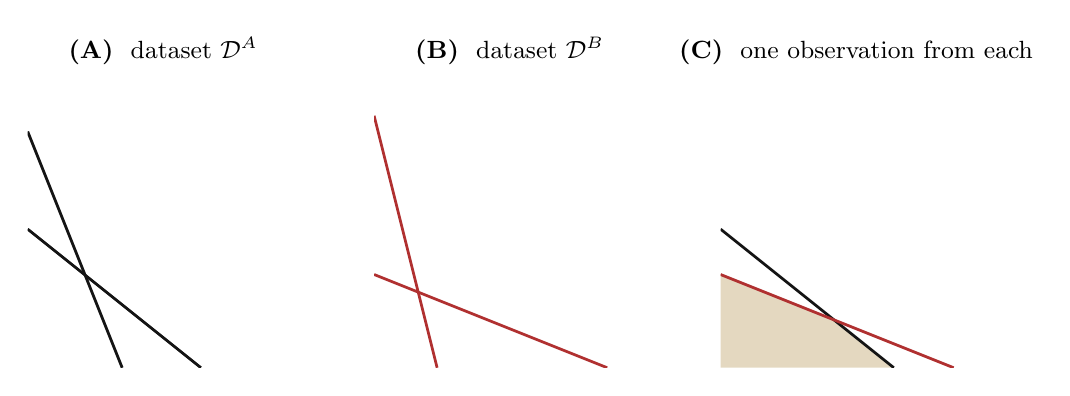
\begin{tikzpicture}[x=0.40cm, y=0.40cm]
\begin{scope}
  \begin{scope}
    \clip (0,0) rectangle (8.6,8.6);
    \draw[groupc, line width=1pt] (0,4.4) -- (5.5,0);
    \draw[groupc, line width=1pt] (0,7.5) -- (3,0);
  \end{scope}
  \panelframe
  \ptmk{4.1905}{1.0476}{groupc}
  \ptmk{1.1538}{4.6154}{groupc}
  \node[font=\small, anchor=south] at (4.3,9.3) {\textbf{(A)}\ \ dataset $\mathcal{D}^{A}$};
\end{scope}
\begin{scope}[xshift=4.4cm]
  \begin{scope}
    \clip (0,0) rectangle (8.6,8.6);
    \draw[memi, line width=1pt] (0,2.96) -- (7.4,0);
    \draw[memi, line width=1pt] (0,8) -- (2,0);
  \end{scope}
  \panelframe
  \ptmk{2.6331}{1.9067}{memi}
  \ptmk{1.3}{2.8}{memi}
  \node[font=\small, anchor=south] at (4.3,9.3) {\textbf{(B)}\ \ dataset $\mathcal{D}^{B}$};
\end{scope}
\begin{scope}[xshift=8.8cm]
  \begin{scope}
    \clip (0,0) rectangle (8.6,8.6);
    \fill[sand] (0,0) -- (0,2.96) -- (3.6,1.52) -- (5.5,0) -- cycle;
    \draw[groupc, line width=1pt] (0,4.4) -- (5.5,0);
    \draw[memi, line width=1pt] (0,2.96) -- (7.4,0);
  \end{scope}
  \panelframe
  \ptmk{4.1905}{1.0476}{groupc}
  \ptmk{2.6331}{1.9067}{memi}
  \node[font=\small, anchor=south] at (4.3,9.3) {\textbf{(C)}\ \ one observation from each};
\end{scope}
\end{tikzpicture}

\begin{minipage}{\textwidth}
\vspace{6pt}
{\footnotesize \emph{Notes}: The dashed diagonal is the certainty line. Panels (A) and (B) each plot two choices, with budget lines and chosen payoff vectors, and each dataset satisfies GARP on its own. In Panel (C), which gathers one observation from each dataset, the shaded region is the set of payoff vectors that are affordable at both budgets. Both chosen payoff vectors lie inside it, so each payoff was affordable when the other was chosen. Thus, WARP is violated. Note that no choice violates first-order stochastic dominance.}
\end{minipage}
\end{figure}

In our experiment, each group is a pair of subjects. Fix a pair $g$ with members $N = {i,j}$, and let $\mathcal{D}^{i}$, $\mathcal{D}^{j}$, and $\mathcal{D}^{g}$ be the datasets of the two members' individual choices and of the pair's collective choices. For $S \subseteq N$, let $\mathcal{D}^{Sg} = \bigl( \bigcup_{m \in S} \mathcal{D}^{m} \bigr) \cup \mathcal{D}^{g}$ denote the merged dataset. By construction, each observation of $\mathcal{D}^{Sg}$ comes either from the individual dataset $\bigcup_{m \in S} \mathcal{D}^{m}$ or from the group dataset $\mathcal{D}^{g}$.

If $\mathcal{D}^{Sg}$ satisfies GARP, one utility function rationalizes the group's dataset together with those of the members in $S$. If not, each $e$-violation of $\mathcal{D}^{Sg}$ is supported either within one of the two datasets or across both. A violation supported within one dataset carries no information about the relation between the members and the group: within $\mathcal{D}^{g}$, it records an inconsistency of the group itself, while within the individual dataset, it records an inconsistency of a member or a disagreement among the members. By contrast, a violation involving observations from both datasets reflects a conflict between the members in $S$ and the group, and these are the violations our measure counts.

\begin{definition}\label{def:cross}\normalfont
An $e$-violation of $\mathcal{D}^{Sg}$ is \emph{cross} if its support contains observations from both the individual dataset $\bigcup_{m \in S} \mathcal{D}^{m}$ and the group dataset $\mathcal{D}^{g}$, and \emph{within-dataset} otherwise.
\end{definition}

Our measure of disagreement applies the logic of the CCEI to cross violations alone, asking how much the budgets must be contracted before all cross violations disappear.

\begin{definition}\label{def:cost}\normalfont
For $S \subseteq N$, the \emph{cross-consistency threshold} of $\mathcal{D}^{Sg}$ is defined as
\begin{align*}
e^{\times}_{Sg} = \sup\bigl\{ e \in (0,1] : \mathcal{D}^{Sg} \text{ admits no cross } e\text{-violation} \bigr\}.
\end{align*}
The corresponding \emph{cross-consistency cost} of $\mathcal{D}^{Sg}$ is $c_{Sg} = 1 - e^{\times}_{Sg}$.
\end{definition}

The cost $c_{Sg}$ is the analogue of $1 - e^{*}$, excluding within-dataset violations. It has a direct expenditure interpretation: $c_{Sg}$ is the smallest fraction by which all budgets must be uniformly contracted to eliminate all cross violations. Thus, $c_{Sg} = 0$ means that the choices of the members in $S$ and the group generate no cross violation, while a larger $c_{Sg}$ indicates a more severe disagreement, in the sense that a larger reduction in expenditure is required to restore cross-consistency. In \autoref{fig:rp_example_v8}, if $\mathcal{D}^{A}$ is the group's dataset and $\mathcal{D}^{B}$ is member $i$'s, the violation in panel (C) is cross and is the only violation of the merged dataset, and so $c_{ig}$ measures the cost of eliminating that single conflict. Increasing $S$ adds observations to the individual dataset and removes none, so cross violations can only accumulate and the cost weakly increases.

\begin{lemma}\label{lem:game}
$c_{\varnothing g} = 0$, and $c_{Sg} \leq c_{S'g}$ whenever $S \subseteq S' \subseteq N$.
\end{lemma}

\autoref{lem:game} gives the collection of costs $\{c_{Sg}\}_{S \subseteq N}$ the structure of a monotone cost game. The total cost $c_{Ng}$ captures the disagreement revealed when both members' datasets are considered together with the group dataset. Our next step is to define a cost-sharing rule that attributes this total cost to the two members according to their respective contributions to it.

A cost-sharing rule assigns the total cost of a cost game to its members. A member's marginal contribution is the additional cross-consistency cost generated by adding her dataset to a given merged dataset. We consider three standard axioms. Efficiency requires that the two cost shares sum to $c_{Ng}$. Symmetry requires that two members with the same marginal contributions receive equal shares. Marginality requires that a member's share depend only on the marginal costs generated by adding that member's dataset.

\begin{proposition}\label{prop:shapley}
The three axioms uniquely determine the following cost-sharing rule:
\begin{align*}
\varphi_{ig} = \tfrac{1}{2} c_{ig} + \tfrac{1}{2}\bigl( c_{Ng} - c_{jg} \bigr) \quad \text{and} \quad \varphi_{jg} = \tfrac{1}{2} c_{jg} + \tfrac{1}{2}\bigl( c_{Ng} - c_{ig} \bigr).
\end{align*}
\end{proposition}

The resulting rule is the Shapley value. For member $i$, the two terms in $\varphi_{ig}$ are her marginal contributions under the two possible orders in which the members' datasets can be merged into the group dataset: $c_{ig}$ when $i$ is added first and $c_{Ng} - c_{jg}$ when $i$ is added second. The Shapley value averages these two contributions. This characterization is due to \citet{young1985monotonic}, and each axiom has a natural interpretation in terms of the data. Efficiency requires the shares to exhaust the pair's revealed disagreement with the group, so the cost-sharing rule is a decomposition of the total cost among the members. Symmetry requires that members be distinguished only by their choices. Thus, two members whose datasets conflict with the group's choices in the same way receive the same cost share, regardless of their identities. Marginality requires that a member answer only for the conflicts her own dataset adds, so her share is identified by comparing the merged data with and without her choices and does not move with disagreement in which her choices play no part. The dummy property follows, so a member whose dataset adds no cross violation at any stage receives a share of zero.

The total cost $c_{Ng}$ varies across pairs, so the cost shares from Proposition 1 are not directly comparable across pairs. Thus, we normalize each member’s share by the pair’s total cost.

\begin{definition}\label{def:index}\normalfont
Suppose $c_{Ng} > 0$. Then, the \emph{revealed-preference distance index} of member $i$'s dataset from the group dataset is
\begin{align}\label{eqn:I_ig}
I_{ig} = \frac{\varphi_{ig}}{c_{Ng}} = \frac{\tfrac{1}{2}\, c_{ig} + \tfrac{1}{2}\bigl( c_{Ng} - c_{jg} \bigr)}{c_{Ng}},
\end{align}
and $I_{jg}$ is defined symmetrically. If $c_{Ng} = 0$, then the index is undefined.\footnote{In our sample, $c_{Ng}$ is zero only 24 groups, making less than 2\% of the analysis sample.
%24total 1,204 pair-level observations. %(8 baseline, 16 endline, 24/1204=0.019=2\%).
}
\end{definition}

The index expresses each member's cost share relative to the pair's total cross-consistency cost. The following proposition summarizes its basic properties.

\begin{proposition}\label{prop:properties}
Suppose $c_{Ng} > 0$. Then, the following hold.
\begin{enumerate}
\item[(i)] $I_{ig} + I_{jg} = 1$ and $I_{ig} \in [0,1]$.
\item[(ii)] $I_{ig} \geq I_{jg}$ if and only if $c_{ig} \geq c_{jg}$.
\item[(iii)] If no cross $e$-violation of $\mathcal{D}^{Ng}$ for any $e \in (0,1]$ involves member $i$'s dataset, then $I_{ig} = 0$.\footnote{The converse need not hold, and an example is provided in the appendix.}
\end{enumerate}
\end{proposition}

The proposition gives the index a simple interpretation. A lower $I_{ig}$ means that member $i$ accounts for a smaller share of the pair's total cross-consistency cost, so the group's choices lie closer to her revealed preferences. Thus, the index captures whose revealed preferences the group's choices more closely follow, without imposing any structure on the deliberation that produced those choices.

We close this subsection with two remarks. First, our construction of the index is not specific to a group of two members. Although we state the index for $|N|=2$ to match our data, the same construction applies to any finite set of members $N$. In this case, \autoref{lem:game} yields a monotone cost game, \autoref{prop:shapley} pins down the cost-sharing rule, and the normalized index of member $m$ is $I_{mg} = \tfrac{\varphi_{mg}}{c_{Ng}}$. \autoref{prop:properties} also extends to this setting. For example, part (i) holds with $I_{ig} + I_{jg}$ replaced by the sum of the shares of all members.

Second, the construction can also be defined using inconsistency measures other than CCEI. Note that CCEI is used only to assign a cost to the cross violations of a merged dataset. Replacing it with the largest money-pump cost of a cross violation \citep{echenique2011money} or the Houtman--Maks index \citep{houtman1985determining} leaves \autoref{lem:game} intact; consequently, our index can be defined analogously. Formal statements, together with an example of an inconsistency measure to which the construction does not apply, are provided in the appendix.

\paragraph{Refinement of the Index} By discarding violations that arise entirely within either the individual or collective dataset and retaining only cross violations, our revealed-preference distance index isolates disagreement across the two sides. But because both individual CCEI and the distance index are derived from revealed-preference comparisons, the choices of a higher-CCEI individual may be mechanically closer to collective choices. 

To this end, we further refine our revealed preference distance measure by constructing a placebo distance measure. %We first randomly match each pair to the group choices of each of all other pairs from the same wave and class. Both members of the original pair are matched to the same placebo group at a time. We retain the members' original individual choices and whether they have higher or lower CCEI within the pair, but recompute the revealed-preference distance index using the reassigned group choices. 
To formally define the placebo distance measure, for each pair $g=(i,j)$ in wave $t$, let $\mathcal{G}_t(g)$ denote the set of
all other pairs observed in the same wave. For each donor pair
$g'\in\mathcal{G}_t(g)$, we retain members $i$ and $j$'s individual choices
but replace their own pair's collective choices with the collective choices
of donor pair $g'$.\footnote{When the donor-specific placebo distance is undefined because the total cross-consistency cost is zero, we set it to $0.5$. Results excluding such donors are nearly identical.} We then recompute the revealed-preference distance and
denote member $i$'s resulting placebo distance by
$\widetilde I_{ig}(g')$. For each pair, we compare both members with the same set of unrelated collective choices, so that their placebo benchmarks continue to sum to one.

We define member $i$'s mean placebo benchmark as
\begin{equation}\label{eq:placebo}
M_{ig}
=
\frac{1}{|\mathcal{G}_t(g)|}
\sum_{g'\in\mathcal{G}_t(g)}
\widetilde I_{ig}(g').
\end{equation}

In the following analysis, we either use the placebo-normalized revealed-preference distance $
I^*_{ig}=I_{ig}-M_{ig}$ or control for $M_{ig}$ to examine whether individual CCEIs explain the revealed preference index above and beyond the mechanical dependency.  Because the same donors are used for both members, $M_{ig}+M_{jg}=1$ and $I^*_{ig}+I^*_{jg}=0$. A negative value of $I^*_{ig}$ therefore means that the collective choices of member $i$'s own pair are more closely aligned with her individual choices than would be predicted by her relative alignment with other pairs' collective choices.
 
 
%%%%%%%%%


\subsection{Collective Rationalizability}
\label{subsec:collective_rationalizability}

We now ask whether the group's choices can be explained by the members' preferences. Specifically, we ask whether the group's choices maximize a weighted sum of two utility functions, each of which must also rationalize the corresponding member's individual choices. We consider two cases: either the weight may vary across collective decisions, or it must remain constant.

Let $s=1,\ldots,N_m$ index member $m$'s choices and $t=1,\ldots,T$ index the group's choices. For $\bar e_m\in(0,1]$, let $\mathcal U_m(\bar e_m)$ be the set of continuous, concave, and strictly increasing utility functions that rationalize member $m$'s choices at efficiency level $\bar e_m$; that is, for every $s=1,\ldots,N_m$, $u_m(x_m^s)\geq u_m(y)$ whenever $y\in\mathbb R_+^2$ and $p_m^s\cdot y\leq\bar e_m$. Note that $\mathcal U_m(\bar e_m)\neq\varnothing$ whenever $\bar e_m$ is strictly smaller than member $m$'s CCEI, and also at the CCEI itself when it is attained. Holding these individual restrictions fixed, we contract the group's budgets as in the definition of the CCEI. For $\eta\in(0,1]$, we say that the group's choices are \emph{Pareto efficiently rationalizable with varying weights (PERVW) at level $\eta$} if there exist $u_i\in\mathcal U_i(\bar e_i)$, $u_j\in\mathcal U_j(\bar e_j)$, and weights $a_t\in(0,1)$ such that, for every $t$,
\begin{align}\label{eqn:collv2_fit}
a_t u_i(x^t)+(1-a_t)u_j(x^t)\geq a_t u_i(y)+(1-a_t)u_j(y)
\quad\text{whenever}\quad y\in\mathbb R_+^2 \text{ and } p^t\cdot y\leq\eta .
\end{align}
We say that the group's choices are \emph{Pareto efficiently rationalizable with a constant weight (PERCW) at level $\eta$} if, in addition, $a_t=a\in(0,1)$ for all $t$.\footnote{For the index values defined below, restricting the weights to $(0,1)$ is without loss of generality. Allowing weights of $0$ and $1$ leaves both suprema unchanged, so the varying-weight index also covers the case in which the members take turns deciding, whereas a constant endpoint weight assigns every decision to the same member. This equivalence concerns only the index values: exact rationalizability at a given $\eta$ may require an endpoint weight. The proof is given in the appendix.}

We now define the measures:
\begin{definition}\label{def:collv2_indices}\normalfont
Conditional on the specified individual calibrations, define
\begin{align}
\mathrm{CEIV}_g(\bar e_i,\bar e_j) &= \sup\{\eta\in(0,1] \vert \text{the choice data is PERVW at level $\eta$} \}, \nonumber \\
\mathrm{CEIC}_g(\bar e_i,\bar e_j) &= \sup\{\eta\in(0,1] \vert \text{the choice data is PERCW at level $\eta$} \}.
 \label{eqn:collv2_indices}
\end{align}
\end{definition}
The two indices have the same expenditure interpretation as the CCEI. One minus each index is the infimum budget contraction needed to rationalize the collective choices by the corresponding weighted sum. 

\begin{figure}[ht]
\centering
\caption{Individual Preferences and a Collective Choice}
\label{fig:collv2_mrs}
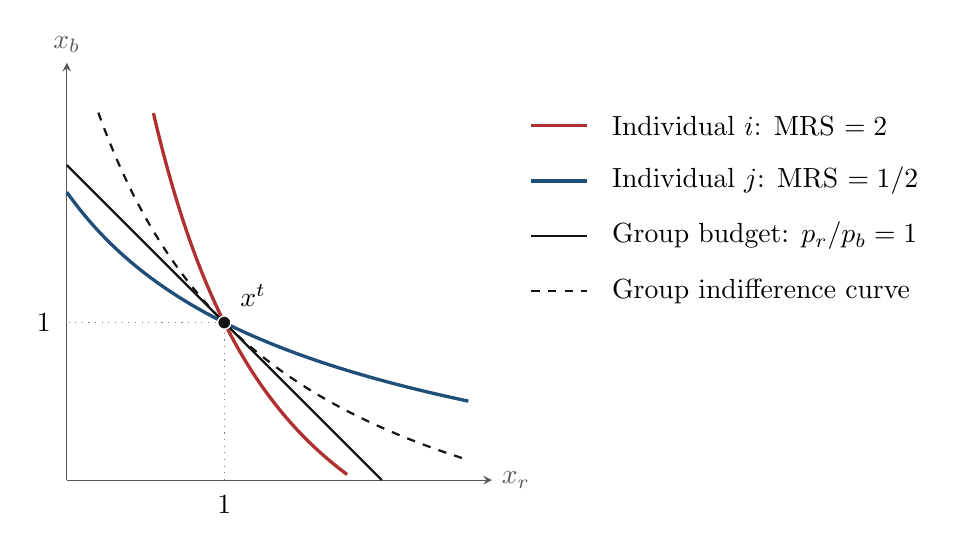
\begin{tikzpicture}[x=2cm,y=2cm,>=stealth,font=\fontsize{10}{12}\selectfont]
  \draw[->,black!65] (0,0) -- (2.7,0) node[right] {$x_r$};
  \draw[->,black!65] (0,0) -- (0,2.65) node[above] {$x_b$};
  \draw[groupc,thick] (0,2) -- (2,0);
  \draw[memi,very thick,domain=0.55:1.78,samples=100]
    plot (\x,{8/((1+\x)^2)-1});
  \draw[memj,very thick,domain=0:2.55,samples=100]
    plot (\x,{sqrt(8/(1+\x))-1});
  \draw[groupc,thick,dashed,domain=0.2:2.55,samples=100]
    plot (\x,{4/(1+\x)-1});
  \draw[dotted,gray] (1,0) -- (1,1) -- (0,1);
  \filldraw[fill=groupc,draw=white,line width=.5pt] (1,1) circle (2.4pt);
  \node[anchor=south west] at (1.04,1.04) {$x^t$};
  \node[anchor=north] at (1,-.04) {$1$};
  \node[anchor=east] at (-.04,1) {$1$};
  \draw[memi,very thick] (2.95,2.25) -- (3.30,2.25);
  \node[anchor=west] at (3.4,2.25) {Individual $i$: MRS $=2$};
  \draw[memj,very thick] (2.95,1.90) -- (3.30,1.90);
  \node[anchor=west] at (3.4,1.90) {Individual $j$: MRS $=1/2$};
  \draw[groupc,thick] (2.95,1.55) -- (3.30,1.55);
  \node[anchor=west] at (3.4,1.55) {Group budget: $p_r/p_b=1$};
  \draw[groupc,thick,dashed] (2.95,1.20) -- (3.30,1.20);
  \node[anchor=west] at (3.4,1.20) {Group indifference curve};
\end{tikzpicture}
%\begin{minipage}{\textwidth}
%\vspace{6pt}
%{\footnotesize\emph{Notes}: $u_i(x)=2\log(1+x_r)+\log(1+x_b)$, $u_j(x)=\log(1+x_r)+2\log(1+x_b)$, and $a_t=1/2$. At $x^t=(1,1)$, the collective indifference curve is tangent to $(x_r+x_b)/2=1$. The Lindahl split is $\pi_i^t=(1/3,1/6)$ and $\pi_j^t=(1/6,1/3)$, summing to $p^t=(1/2,1/2)$. The picture concerns exact rationalization at an interior choice; contracted comparison budgets do not require tangency at the observed bundle.}
%\end{minipage}
\end{figure}

Notably, only the group budgets are contracted, while the individual utility functions remain fixed and all observations are retained. \autoref{fig:collv2_mrs} illustrates the restriction on the members' utility functions. For this illustration, we assume that $u_i$ and $u_j$ are differentiable and that $x^t\gg0$ maximizes their weighted sum on the original group budget ($\eta=1$). The first-order condition is $
a_t\nabla u_i(x^t)+(1-a_t)\nabla u_j(x^t)=\kappa_t p^t$ for some $\kappa_t>0$. The group's willingness to trade must lie between the two individuals' willingness to trade, evaluated at the group bundle $x^t\gg0$. To see this, let $\mathrm{MRS}_m=\partial_r u_m/\partial_b u_m$ and write the condition as
\begin{align*}
\frac{p_r^t}{p_b^t}
 =\theta_t\mathrm{MRS}_i(x^t)+(1-\theta_t)\mathrm{MRS}_j(x^t),
\qquad
\theta_t=\frac{a_t\partial_bu_i(x^t)}{a_t\partial_bu_i(x^t)+(1-a_t)\partial_bu_j(x^t)}.
\end{align*}
The weight $\theta_t$ depends on the members' marginal utilities at the chosen bundle, so it may vary even when the aggregation weight $a_t$ is constant.

The following proposition gives conditions for collective rationalizability that can be tested on the observed data, without assuming differentiability. Let $\mathcal R_m$ index the individual and collective bundles for member $m$, with $z_m^s=x_m^s$ and $z_m^{g_t}=x^t$.

\begin{proposition}\label{prop:collv2_afriat}
Fix $\eta\in(0,1]$ and $(\bar e_i,\bar e_j)$. The following are equivalent:
\begin{enumerate}
\item[(i)] The group choice is PERVW.
\item[(ii)] There exist $v_m^r,\beta_m^t\in\mathbb R$, $\lambda_m^s,\kappa_t>0$, $h_m^t\gg0$, and $a_t\in(0,1)$, such that
\begin{align}
v_m^r&\leq v_m^s+\lambda_m^s(p_m^s\cdot z_m^r-\bar e_m),&&\forall m,s,r,\label{eqn:collv2_I}\\
v_m^r&\leq\beta_m^t+h_m^t\cdot z_m^r,&&\forall m,t,r,\label{eqn:collv2_S}\\
a_th_i^t+(1-a_t)h_j^t&=\kappa_t p^t,&&\forall t,\label{eqn:collv2_P}\\
a_t\beta_i^t+(1-a_t)\beta_j^t+\kappa_t\eta
&\leq a_tv_i^{g_t}+(1-a_t)v_j^{g_t},&&\forall t.\label{eqn:collv2_B}
\end{align}
\end{enumerate}
\begin{enumerate}
\item[(iii)] There exist personalized prices $\pi_m^t\gg0$ and expenditures $\tau_m^t$ with
\begin{align*}
\pi_i^t+\pi_j^t=p^t,\qquad
\tau_i^t+\tau_j^t=\eta,\qquad
0<\tau_m^t\leq\pi_m^t\cdot x^t,
\end{align*}
such that each augmented dataset
\begin{align*}
\widetilde{\mathcal D}_m
=\{(p_m^s,x_m^s,\bar e_m)\}_{s=1}^{N_m}
\cup\{(\pi_m^t,x^t,\tau_m^t)\}_{t=1}^{T}
\end{align*}
satisfies adjusted GARP. A row $(P,z,w)$ reveals $z$ weakly preferred to $z'$ if $P\cdot z'\leq w$, strictly if $P\cdot z'<w$; adjusted GARP excludes a directed cycle with a strict comparison.
\end{enumerate}
\end{proposition}

Part (iii) gives the revealed-preference interpretation of CEIV. Each collective choice is added to both members' datasets, with personalized prices that sum to the market price. The augmented data must satisfy GARP for each member. These personalized prices are Lindahl prices: they support the same collective bundle from the perspective of each member and need not describe actual payments. In the differentiable case illustrated above, $\pi_i^t=a_t\nabla u_i(x^t)/\kappa_t$ and $\pi_j^t=(1-a_t)\nabla u_j(x^t)/\kappa_t$. The expenditures $\tau_m^t$ allow the two members' comparison budgets to contract by different proportions.

%These indices assume that the members' preferences remain the same between individual and collective decisions. A low value may therefore reflect a change in preferences or noise in the individual data, as well as a failure of the collective model. The indices also depend on the individual calibrations. Holding the observations fixed, lowering either calibration allows more utility functions and hence weakly increases both indices. A relation between these indices and the members' CCEIs may therefore partly arise from the calibration rule, although this does not determine the sign of a regression coefficient because choices also differ across groups. As with the CCEI, an index of one need not imply exact rationalizability on the original budgets, since the supremum may not be attained.

\noindent \textbf{Remarks.} Our measure builds on revealed-preference tests of collective consumption \citep{cherchye2007,cherchye2011}. In particular, \citet{cherchye2020caring} use individual and joint choices to test a collective model with stable individual preferences, and \citet{bruyneel2012restricted} compare models with different restrictions on bargaining weights. We allow for inconsistency in the individual choices using each member's CCEI and then measure how much the group budgets must be contracted for a collective explanation. Both members evaluate the same group payoff vector. In this setting, any finite group dataset can be rationalized if the members' utilities are unrestricted. The individual data therefore make the model testable.

The relation between the three group indices follows from their definitions. A constant weighted sum is a special case of a varying weighted sum, and it is also a single utility function that rationalizes the group dataset. Thus, suppressing the individual calibration arguments,
\begin{align}
\mathrm{CEIC}_g\leq\min\{\mathrm{CCEI}_g,\mathrm{CEIV}_g\}.
\label{eqn:collv2_order}
\end{align}
Group CCEI and CEIV need not be ordered. The former requires a single group utility, while the latter requires compatibility with the individual choices but allows the aggregation weight to vary. CEIC may also be strictly smaller than both.\footnote{\autoref{app:collv2_examples} gives examples with $(\mathrm{CCEI}_g,\mathrm{CEIV}_g,\mathrm{CEIC}_g)=(1/2,1,1/2)$ and $(1,1/2,1/2)$; in the latter, the collective supremum is not attained. A third example has individual CCEIs, group CCEI, and CEIV all equal to one, but CEIC strictly below one.} The difference CEIV$-$CEIC therefore measures how much more of the group budgets can be retained when the weight is allowed to change. It does not measure the size of changes in the weight, which is not identified by these indices.

%%%%%%%%%

%\subsection{Risk Aversion}\label{subsec:risk_aversion}

%Our analysis also uses a simple nonparametric measure of risk attitude, both to describe choices and to compare preferences within a pair. For each observation $k$, let $ra^{k}$ denote the demand share of the more expensive security, so that $ra^{k} = \tfrac{x^{k}_{r}}{x^{k}_{r}+x^{k}_{b}}$ when $p^{k}_{r} > p^{k}_{b}$ and $ra^{k} = \tfrac{x^{k}_{b}}{x^{k}_{r}+x^{k}_{b}}$ when $p^{k}_{b} > p^{k}_{r}$. Since the two states are equally likely, a risk-neutral or risk-seeking decision maker buys only the cheaper security and obtains $ra^{k} = 0$, an extremely risk-averse one buys the fully insured payoff and obtains $ra^{k} = \tfrac{1}{2}$, and any decision maker who respects first-order stochastic dominance obtains $ra^{k} \in [0, \tfrac{1}{2}]$. Averaging $ra^{k}$ across a subject's 18 individual purchases gives the individual measure $RA_{i}$, and averaging across a pair's 18 collective purchases gives the group measure $RA_{g}$.

%%%%%%%

\section{Data Description and Balance Check}

This section establishes the empirical foundation for the analyses that follow. We first describe the distributions of the experimental measures introduced in \autoref{sec:measurement}. In particular, variation in CCEIs and revealed-preference distance suggest a scope to examine how these are related. 

Next, the specification and interpretation developed in the previous section relies on the random assignment of partners. Our fixed-effects analysis also relies on within-individual changes among students observed in both waves. Selective attrition could distort the relationship between changes in individual rationality and group decision outcomes by determining which individuals and pairs remain in the sample. We therefore assess the implementation of within-class random assignment and examine whether inclusion in the analysis sample is associated with baseline rationality and other individual characteristics.


\subsection{Summary Statistics}
\autoref{tab:ccei_summary} reports summary statistics for the measures constructed in \autoref{sec:measurement}, separately for the two waves. The mean individual CCEI is 0.900 at baseline and 0.932 at endline, and the mean group CCEI is 0.912 and 0.936, respectively. These values are comparable to those reported in prior portfolio-choice experiments: \citet{Choietal:2007:AER} and \citet{Choietal:2014:AER} report mean individual CCEIs of 0.881 and 0.954, while \citet{GonzalezJimenezMueller2025SSRN} report a mean CCEI of 0.926 for choices made by pairs. There is substantial dispersion in both individual and group CCEIs, with the standard deviation ranges from 0.12 to 0.14; the analysis below exploits this heterogeneity in individual and group decision-making quality. Mean individual risk aversion $RA_{i}$ is 0.322 at baseline and 0.297 at endline; the corresponding group means, 0.297 and 0.265, are slightly lower.\footnote{See \autoref{fig:cdf_ind_group_ccei} and \autoref{fig:cdf_ind_group_ra} for the full distributions of these measures.}\footnote{Pooling both waves, 20.8\% of the 70,416 individual and collective choices in the main analysis sample violate first-order stochastic dominance, counting each collective choice once. A violation occurs when more of the strictly more expensive security is purchased.} The mean and standard deviation of group CEIVs are 0.924, 0.946 and 0.118, 0.109 in baseline and endline, respectively, showing that pairs overall choices whose deviation from efficiency is moderate but also there is substantial heterogeneity across pairs.

\begin{table}[h]
\centering
\caption{Summary Statistics Of Experimental Measures}
\label{tab:ccei_summary}
\begin{tabular}{lcccccc}
\toprule \hline
\input{tables_2025/table_ccei_summary_IminusM}
\end{tabular}
\begin{minipage}{\textwidth}
{\footnotesize \emph{Notes}: Individual measures are reported at the student-wave level; group measures are reported at the pair-wave level. Risk aversion is the average demand share of the more expensive Arrow security. CCEI is the Critical Cost Efficiency Index, described in \autoref{subsec:rationality}. CEIV is the varying-weight collective rationalizability index, described in \autoref{subsec:collective_rationalizability}. The placebo-adjusted distance is $I^*_{ig}=I_{ig}-M_{ig}$, where $M_{ig}$ is the mean placebo benchmark in \autoref{eq:placebo}, averaging distances to all 651 non-own pairs in the same wave and assigning undefined donor distances one half. Its number of observations is smaller because actual distance $I_{ig}$ is undefined when the denominator in \autoref{eqn:I_ig} is zero.}
\end{minipage}
\end{table}

The placebo-adjusted revealed-preference distance $I^*_{ig}=I_{ig}-M_{ig}$ has a mean of 0.000 in both waves. Both actual distance and the placebo benchmark sum to one within a pair, so the two adjusted distances sum to zero and the pooled mean is zero by construction. The dispersion statistics are more informative. The standard deviation is 0.247 at baseline and 0.302 at endline, and the tenth and ninetieth percentiles are $-0.326$ and $0.326$ at baseline and $-0.413$ and $0.413$ at endline. Negative values indicate that a member's own group choices are closer to her individual choices than the placebo benchmark predicts; positive values indicate the reverse. These statistics use the 1,288 student-wave observations with defined actual distance at baseline and 1,272 at endline. \autoref{fig:hist_bargaining_index} in the appendix reports the pooled distributions separately for higher- and lower-CCEI members.
\autoref{section:results} examines whether this dispersion in revealed-preference distance is systematically related to individual rationality and other individual characteristics.

%%%%%%%%%%

\subsection{Empirical Specification}
We next present our empirical specifications and explain how we interpret the coefficients of interest.

First, to examine how individual rationality relates to revealed-preference distance between individual and group choices in \autoref{sec:main_results}, we estimate the following regression equation:

\begin{align}\label{eqn:individual_distance}
I_{igt} = \alpha + \beta_1\, Higher CCEI_{it} + \rho M_{igt} + X'_{igt} \gamma + \tau_c + \varepsilon_{ict},
\end{align}
The indicator $Higher CCEI_{it}$ equals one if individual $i$'s CCEI is at least as high as her partner's at time $t$ and zero otherwise. When the two members have identical individual CCEIs, both are classified as higher-CCEI members. There are 174 pair-wave observations with ties, comprising 13.9\% of the 1,256 pair-wave observations in the balanced revealed-preference-distance regression sample used in \autoref{tab:pref_agg_ccei}. Alternatively, we also estimate a regression equation where we replace $Higher CCEI_{it}$ with the $CCEI_{it}-CCEI_{-it}$, which is the difference between the individual's CCEI and their partner's CCEI. $M_{igt}$ is the mean placebo distance defined in \autoref{eq:placebo}, and we let the data decide its coefficient, $\rho$. $X_{igt}$ includes individual observable characteristics, within-pair differences in those characteristics, gender composition of the pair, and furthermore friendship-network controls. Missing values in math scores and Big Five traits are imputed with zeros, and corresponding missing indicators are included. The pooled specifications include class fixed effects $\tau_c$, and standard errors are clustered at the class level.

With partners randomly assigned, our estimate of $\beta_1$ tells us whose revealed preferences their collective choices more closely follow when individuals with different levels of rationality come together to make decisions. Random assignment of partners rules out any biases in $\beta_1$ that can arise from endogenous partner selection: more rational individuals cannot systematically choose partners who are especially receptive to their suggestions or with whom they have already established a decision-making protocol.

Taking this question one step further, one might ask whether $\beta_1$ captures an effect attributable to rationality as measured by CCEI or a combined effect involving other individual characteristics. For example, more rational individuals may also have greater cognitive ability, and both features may help explain why collective choices follow their preferences. Our primary question concerns individuals with the characteristics that naturally accompany their measured rationality. From this perspective, correlations between CCEI and other characteristics are part of the phenomenon of interest. Our estimate of $\beta_1$ remains informative about whose revealed preferences collective choices follow when individuals with different levels of rationality make decisions together, to the extent that the associations between CCEI and other characteristics remain comparable.

Nevertheless, examining what CCEI captures beyond other characteristics helps clarify the content of measured rationality and how changes in rationality might translate into changes in collective choices. We pursue this question in two ways. First, we include observable individual and pair characteristics in $X$. These controls also include the frequency of corner and equal-allocation choices. Although such decision rules are one form of making rational decisions, these may be particularly easy to communicate to a partner. Controlling for these patterns allows us to assess whether relative rationality remains informative beyond these specific forms of choice behavior.

Second, we exploit the two-wave panel to examine whether changes in relative rationality within the same pair are accompanied by changes in revealed-preference distance. To this end, we replace class fixed effects in Equation~\eqref{eqn:individual_distance} with individual fixed effects and omit time-invariant controls. This specification absorbs stable individual characteristics, both observable and unobservable, such as persistent confidence and communication ability. It provides a demanding test by removing all between-individual variation. Under the assumption that changes in relative rationality are unrelated to unobserved changes affecting group decisions conditional on observed changes, one can interpret $\beta_1$ as the causal effect on revealed-preference distance attributable to relative rationality as measured by CCEI, rather than the confounding influence of other individual characteristics.

Moving onto the question on how both members' rationalities affect the quality of group decision making,  we estimate the following regression to quantify the connection between group CCEI and the two members' CCEIs, conditional on observed individual and pair characteristics:
\begin{align}\label{eqn:CCEI_reg}
CCEI_{gct} = \alpha + \beta_1\, CCEI_{max,gt} + \beta_2\, CCEI_{min,gt} +  X'_{gt}\gamma + \tau_c + \varepsilon_{gct},
\end{align}
where $CCEI_{gct}$ is the CCEI of pair $g$ in class $c$ at time $t$, $\text{CCEI}_{\text{max},gt}$ is the larger of the two individual CCEIs, $\text{CCEI}_{\text{min},gt}$ is the smaller of the two individual CCEIs, $X_{gt}$ includes within-pair characteristics (gender composition, height, math scores, Big Five traits, and friendship measures), and $\tau_c$ denotes class fixed effects. Standard errors are clustered at class level.

As discussed above, random assignment of partners rules out endogenous group formation as an explanation for the relationships captured by $\beta_1$ and $\beta_2$. Our primary question again concerns how individuals of varying rationality make collective decisions. To further examine whether these relationships are attributable to rationality as measured by CCEI beyond other individual characteristics, we follow the same two approaches: controlling for observable individual and pair characteristics $X$ and estimating fixed-effects specifications that absorb stable characteristics of the paired individuals.

% what happens to group decision making when individuals of varying rationality come together? To what extent any effect of rationality is attributable rationality per se rather than other individual chracteristics?
\subsection{Randomization Test and Sample Attrition}

Next, we test that the within-classroom random assignment of pairs was successfully implemented, which is the basis for our causal interpretation of how individual characteristics shape group decisions. Specifically, we run the following regression equation:
\begin{align}\label{eqn:randomization}
y_{i} = \beta\, y_{-i} + \tau_{c(i)} + \varepsilon_{ic(i)},
\end{align}
where $y_i$ is the baseline characteristic of one randomly selected member within each pair, $y_{-i}$ is the same characteristic for that member's partner, and $\tau_{c(i)}$ are class fixed effects. Standard errors are clustered at the class level. If randomization was properly implemented, partner characteristics should not predict each other within a pair (i.e., $\beta = 0$). We focus on baseline characteristics because the four-month gap between waves may have allowed initial pairings to affect endline characteristics, for example through friendships formed after exposure to the partner. Columns (1) and (2) of \autoref{tab:attrition_balance} report the randomization test. Across all twelve variable outcomes---two experimental measures (CCEI and risk aversion) and ten survey measures (gender, height, math score, in- and out-degree, and the Big Five traits)---no estimate is statistically significant at the 5\% level. The joint Wald test fails to reject the null that all twelve coefficients are zero ($\chi^{2}(12) = 8.93$, $p = 0.709$).

\begin{table}[h!]
\centering
\caption{Randomization Test and Sample Attrition}
\label{tab:attrition_balance}
\begin{tabular}{lcccccc}
\toprule \hline
\input{tables_2025/table_attrition_balance}
\end{tabular}
\begin{minipage}{\textwidth}
{\footnotesize \emph{Notes}: Columns (1) and (2) report the coefficient and $p$-value from regressions of one randomly selected pair member's baseline characteristic on the partner's corresponding baseline characteristic, controlling for class fixed effects. The randomization-test joint statistic is a Wald test that all twelve partner-characteristic coefficients are jointly zero. Columns (3) and (4) report baseline means for all students who participated in the baseline decision-making experiment and for students in the analysis sample, respectively. Column (5) reports the analysis-sample mean minus the baseline mean. $p$-values in column (6) come from two-sample $t$-tests. For math score and Big Five personality measures, means and attrition $p$-values are computed among students with nonmissing valid values (baseline $N=1,546$; analysis-sample $N=1,286$); all other rows use the full available samples reported in the $N$ row. The same valid-value restriction is used for the corresponding randomization-test regressions. The joint test for sample attrition regresses an indicator for inclusion in the analysis sample on all listed characteristics and tests that all coefficients are jointly zero.}
\end{minipage}
\end{table}


Now, let us turn to sample attrition. The experiment and surveys were administered during regular school days as part of school activities, so wave-to-wave attrition mainly reflects absence or transfer to another school or one student from each odd-numbered class not being assigned to a pair. These leave us 1,425 students who completed the experiment in both waves. Applying the matched-pair and data-cleaning restrictions described in \autoref{sec:data_collection} excludes a further 121 students and leaves a final analysis sample of 1,304 students. \autoref{tab:attrition_balance} compares all baseline experiment participants with the analysis sample. The two samples are similar across experimental and survey measures, and none of the differences is statistically significant at the 5\% level.

Taken together, these checks support the implementation of within-class random assignment and provide no evidence of systematic selection into the analysis sample based on baseline rationality or other observed characteristics.


%%%%%%%%%%%%%%%%%%%
\section{Rationality-based Preference Aggregation}
\label{section:results}
We now use the revealed preference distance to assess whether collective choices are especially close to the individual choices of more rational members.

\subsection{Individual Rationality and Revealed-Preference Distance}\label{sec:main_results}
\autoref{fig:cdf_rp_distance} compares revealed preference distance index by whether the individual subject has larger or smaller CCEI than her partner. Panel (a) reports mean placebo adjusted distance index, $I_{ig}-M_{ig}$, for lower- and higher-CCEI members, pooling both waves. Higher-CCEI members have a substantially lower mean distance, $-0.034$ compared with $0.045$ for lower-CCEI members; the difference between these category means is $0.078$ ($p<0.01$), equal to XXX\% of the pooled standard deviation of this measure. Beyond averages, the CDF for the higher-CCEI member is first-order stochastically dominated by that for the lower-CCEI member (Kolmogorov-Smirnov test: $p<0.01$) as shown in Panel (b). Together, these patterns show that collective choices are closer, in revealed-preference terms, to more rational members' individual choices. These show that when individuals with different levels of rationality come together to make decisions, the collective choices systematically follow the revealed preferences  of the more rational member.


\begin{figure}[h!]
\centering
\caption{Placebo-Adjusted Distance By Members' CCEI}
\label{fig:cdf_rp_distance}
\begin{subfigure}[b]{0.485\textwidth}
\centering
\includegraphics[width=\textwidth]{figures_2025/ccei_IminusM_by_higher_ccei_bar.png}
\caption{Mean Placebo-Adjusted Distance}
\end{subfigure}
\begin{subfigure}[b]{0.485\textwidth}
\centering
\includegraphics[width=\textwidth]{figures_2025/ccei_IminusM_by_higher_ccei_cdf.png}
\caption{CDFs of Placebo-Adjusted Distance}
\end{subfigure}
\vspace{12pt}
\begin{minipage}{\textwidth}
{\footnotesize \emph{Notes}: Both panels use $I^*_{ig}=I_{ig}-M_{ig}$ for the 2,560 student-wave observations with defined actual distance. The benchmark averages distances to all 651 non-own pairs in the same wave, assigning undefined donor distances one half. Both members are classified as higher CCEI in a tie. Panel (a) reports means with 95\% confidence intervals and the higher-minus-lower mean difference; significance is based on a two-sample $t$-test. Panel (b) reports empirical CDFs. Negative values indicate that the member's own group choices are closer to her individual choices than the donor benchmark. +, *, and ** denote $p<0.10$, $p<0.05$, and $p<0.01$, respectively.}
\end{minipage}
\end{figure}


\begin{table}[h!]
\centering
\caption{Individual Rationality and Revealed-Preference Distance from Group Choices}
\label{tab:pref_agg_ccei}
\resizebox{\textwidth}{!}{  
\begin{tabular}{lcccccc}
\toprule \hline
& \multicolumn{3}{c}{Ties Assigned High} & \multicolumn{3}{c}{CCEI Difference} \\
\cmidrule(lr){2-4}\cmidrule(lr){5-7}
Dependent variable: $I_{ig}$ & (1) & (2) & (3) & (4) & (5) & (6) \\ \midrule
\input{tables_2025/table_bargainingCCEI_M}
\end{tabular}}
\begin{minipage}{\textwidth}
{\footnotesize \emph{Notes}: The table reports results from estimating \autoref{eqn:individual_distance}. In Columns (1)--(3), the higher-CCEI indicator equals one for both members when their individual CCEIs are equal. Columns (4)--(6) replace this indicator with $CCEI_i-CCEI_j$. The revealed-preference distance $I_{ig}$ is undefined when the total cost, $c_{Ng}$, is zero; to maintain a common balanced sample across specifications, we retain only pairs for which $I_{ig}$ is defined in both waves, yielding 2,512 student-wave observations from 1,256 students in 628 pairs. Columns (1), (2), (4), and (5) include class fixed effects; Columns (3) and (6) include individual fixed effects. Columns (2), (3), (5), and (6) include individual and friendship characteristics and the member's shares of exact corner and equal-allocation choices, together with their within-pair differences. Risk aversion and its within-pair difference are excluded. Gender-composition controls are included in Columns (2) and (5), with same-sex pairs as the omitted category, and are absorbed by individual fixed effects in Columns (3) and (6). Standard errors are clustered at the class level and presented in parentheses. +, *, ** denote significance at the 10\%, 5\%, and 1\% levels, respectively.}
\end{minipage}
\end{table}


To further ask to what extent individual rationality rather than other characteristics drives the results, we estimate \autoref{eqn:individual_distance} and report the results in \autoref{tab:pref_agg_ccei}. In Columns (1)--(3), the coefficient on $Higher\ CCEI_i$ is negative and statistically significant at the 1\% level. Column (2) adds individual and friendship characteristics and the shares of choices exactly at the corners or at the 50/50 allocation.\footnote{A choice is classified as a corner only if one payoff is exactly zero, and as a 50/50 allocation only if the two payoffs are exactly equal. Appendix \autoref{tab:pref_agg_ccei_buffers} allows buffers of 2.5 and 5 percentage points to allow for "trembling hands".} The latter address the concern that simple choice rules that are easy to communicate might generate both high individual CCEI and lower revealed preference distance, and these choices entirely drive the relationship of interest. Adding the full set of controls increases explanatory power but changes the coefficient only modestly, although individual CCEI is correlated with several of these characteristics (\autoref{tab:corr_ihat}). Furthermore, the relationship between individual rationality and revealed preference is not entirely driven by simple choice rules such as choosing corners or midpoints no matter how the budget set looks like. 

The individual-fixed-effects estimate in Column (3) remains similar, at $-0.090$. This result provides evidence that revealed-preference distance follows relative rationality within the same individual, rather than reflecting only stable unobserved characteristics of more rational individuals within pairs. Thus, we interpret the fixed-effects result as strong evidence that individual rationality per se is systematically related to whose choices are more closely reflected in collective decisions. On whether we have enough variation for the fixed effect specification, the higher-CCEI indicator changes between waves for 42.2\% of individuals in our analysis sample.

Columns (4)--(6) replace the higher-CCEI indicator with $CCEI_i-CCEI_j$. The coefficients are $-0.249$, $-0.228$, and $-0.214$, respectively, and all are significant at the 1\% level. In the individual-fixed-effects specification, a one-standard-deviation increase in the CCEI difference corresponds to a decrease of $0.119$ standard deviations in actual distance, conditional on $M_{ig}$. These results further show that not only whether an individual is more rational than her partner, but also how much more rational conveys information on how close group decisions are more aligned with individual decisions.

Three additional points are worth noting. First, the coefficient is economically and statistically significant, but not $-1$. Thus, although group choices closer to the choices of the higher-CCEI member, the lower-CCEI member's choices also remain reflected in the group decision. Second, the other covariates provide little systematic evidence of other correlates of revealed-preference distance. If anything, math score is the only exception. Individuals with higher math score, when their math score is particularly larger than their partner's, induce group choices to be more aligned with thier choices. In-degree is not consistently related to revealed-preference distance, and the mixed-gender indicators are small and statistically insignificant. A Shorrocks--Shapley decomposition of the regression $R^2$ from Column (3) in \autoref{tab:pref_agg_ccei} shows that the Higher CCEI indicator accounts for XX\% of within-individual variation whereas other observable characteristics accounts only for XX\% (\autoref{fig:shapley_I_ig}). \textcolor{red}{appendix figure XXX also shows a similar pattern when using the distance in CCEI.} Although it is a natural hypothesis to think that the mover status might matter, that is not supported by our results (\autoref{tab:bargaining_ccei_ihat_mover}).
 Finally, the over-time variation in relative rationality is relevant in our setting. A natural concern is that changes in CCEI may reflect measurement noise rather than changes in underlying decision quality. The most direct evidence against a pure-noise interpretation is the individual-fixed-effect estimate itself: random noise in measured CCEI would be unlikely to systematically predict whose choices are more reflected in group deliberation. Although two waves do not allow us to fully decompose this variation into learning, maturation, and measurement error, features of the data help characterize where it may come from. To begin with, the subjects are adolescents, an age at which decision-making ability may still be malleable \citep{kim2018role}. Moreover, Appendix \autoref{tab:individual_ccei_change} shows that gender is the clearest predictor of changes in individual CCEI: boys' CCEI increases by 0.035--0.037 points more than girls' across the two specifications, with both estimates significant at the 1\% level. Column (1) controls for baseline individual characteristics, and Column (2) additionally controls for changes in math score and friendship-network measures. This pattern is consistent with broader evidence that developmental trajectories during adolescence differ by sex \citep{lenroot2010sex}. Among the remaining covariates, only changes in math score are marginally associated with changes in CCEI (coefficient $0.007$, $p=0.067$).

\subsection{Robustness and Sensitivity}
\paragraph{Robustness to Alternative Measures} To assess whether the result depends on this particular measure of revealed-preference inconsistency, we repeat the analysis using two alternatives based on the Houtman--Maks approach \citep{houtman1985determining}, and reversed MaxMPI, based on the maximum money-pump index \citep{echenique2011money}. FGARP records the fraction of observations that can be retained while restoring GARP, whereas MaxMPI records the largest monetary loss generated by a revealed-preference cycle. We reverse MaxMPI so that, as with CCEI and FGARP, higher values indicate greater rationality. For each alternative, we reclassify the higher-rationality member, construct the corresponding revealed-preference distance, and reestimate specifications in \autoref{tab:pref_agg_ccei}.

Alternatively, one can also use a direct analogue of $I_{ig}$ is member $i$'s squared distance from the group's risk aversion, normalized by the sum of two members' squared distances from the group:
\begin{align}\label{eqn:simple_measure}
d(RA_i, RA_g) = \frac{(RA_i - RA_g)^2}{(RA_i - RA_g)^2 + (RA_j - RA_g)^2}.
\end{align}
This index is bounded in $[0, 1]$ and sums to one within a pair, mirroring the structure of $I_{ig}$. It is  coarser, however, because it ignores the full pattern of choices and records how close a member's average risk-aversion measure is to the group's risk aversion. Moreover, any inconsistency in individual choices enters the $RA$ summary as measurement noise rather than as an object of analysis.  The available variation in $RA$ is itself compressed, too: because many subjects choose near the certainty line, their $RA$ values cluster near the upper bound of $1/2$ (See Appendix \autoref{fig:cdf_ind_group_ra} for the distribution of RA). Disappointment-aversion preferences \citep{Gul:1991:ECMA} which generate a kink at the certainty line provide one interpretation of this bunching. For these reasons, we view $d(RA_i, RA_g)$ as a complementary robustness check rather than as an alternative revealed-preference measure.

Appendix \autoref{tab:pref_agg_alternatives} confirms that group decisions are more aligned with individual choices with higher rationality across these alternative measures. In Column (3) of Panel A and B, the higher-rationality coefficients are $-0.083$ for HM and $-0.103$ for RevMaxMPI, equivalent to 34.3\% and 35.3\% of the pooled outcome standard deviations. In Column (6), a one-standard-deviation increase in the rationality difference corresponds to decreases of $0.168$ ($0.259$ standard deviations in \autoref{tab:alternative_indices_summary}). All four estimates are significant at the 1\% level. Panel C uses $d(RA_i,RA_g)$ as the outcome and controls for its own placebo benchmark. All the estimates confirm that group decisions are more aligned with individual choices with higher CCEI, although coefficients in individual fixed effect specifications lose its significance with this coarser outcome.

\paragraph{Validation using Hold-out} Another concern one might have is that the main analysis uses the same individual choice data both to determine which member has the higher CCEI and to construct the revealed-preference-distance outcome. To this end, \textcolor{red}{we construct the individual-rationality and revealed-preference-distance measures from disjoint choices. For each pair-wave observation, we independently divide the 18 choices of each member and the group into two sets of nine. Within each partition, one set is used to determine relative individual rationality and construct the individual choice-based controls, while the other is used to construct revealed-preference distance; we then exchange the roles of the two sets. Repeating this procedure for 500 random partitions yields 1,000 coefficient estimates, which are pooled in \autoref{tab:disjoint_choice}.}

% Retain the old numerical comparison until the complete replacement is exported.
\IfFileExists{tables_2025/table_disjoint_choice.tex}{%
\autoref{tab:disjoint_choice} repeats the six specifications of \autoref{tab:pref_agg_ccei} using disjoint choices. Columns (1)--(3) use the higher-CCEI indicator, assigning ties high, and Columns (4)--(6) use the signed within-pair CCEI difference. Every column controls for a placebo benchmark recomputed from the outcome set of choices. The table reports median coefficients and the 2.5th and 97.5th percentiles of the 1,000 split estimates; the full specifications include the same individual, friendship, and choice-share controls as the main analysis. The balanced sample is determined separately for each partition and direction by requiring defined outcome-set distance in both waves.
}{%
\textcolor{red}{Panel A reports four raw-distance diagnostic specifications using the higher-CCEI indicator: class fixed effects alone, student and friendship controls, full controls, and individual fixed effects. These pre-existing disjoint-choice regressions do not control for $M_{ig}$ and are not re-estimates of the updated main specification. The median coefficients in the four rows are $-0.168$, $-0.164$, $-0.139$, and $-0.082$, respectively. The 95\% ranges for the first three rows lie entirely below zero, whereas the range for the individual-fixed-effects specification in the fourth row, $[-0.205,\,0.026]$, includes zero.}

% TODO: Verify the 46\% tie rate and the disjoint-choice table's estimation vintage; current outputs are missing and the current script's tie treatment differs from the table notes.
\textcolor{red}{Because splitting the choices increases the frequency of ties, the two members have identical half-sample CCEIs in approximately 46\% of comparisons. Panel B therefore uses the continuous within-pair CCEI difference. Specifically, the absolute CCEI difference from one set is used to explain the difference between the two members' revealed-preference distance indices from the other set, defined as the higher-CCEI member's distance minus the lower-CCEI member's distance. The pooled median coefficient is $-0.832$, its 95\% range is $[-1.066,\,-0.586]$, and all 1,000 estimates are negative. Thus, the relationship persists when the choices used to measure individual rationality are disjoint from those used to construct the revealed-preference-distance outcome.}

}

\paragraph{Placebo Tests} As described in section XXX, we refine the revealed preference distance measure by randomly matching pairs and derive and control for a placebo distance measure. If the placebo measure captures all of mechanical dependency, we should see that the effect of individual rationality should vanish when we use revealed distance measure from randomly matched pairs as a dependent variable. 

\textcolor{red}{The placebo regressions results in \autoref{fig:placebo_reassignment_bothhigh} generate negative coefficients, confirming that the construction itself creates some correlation. However, the relationship among actual pairs is substantially stronger. In the unadjusted baseline diagnostic, the actual coefficient is $-0.250$, compared with a median placebo coefficient of $-0.194$; the actual estimate is also more negative than the lower 2.5th percentile of the placebo distribution. The same pattern holds in all four raw-index diagnostic specifications, with the difference between the actual coefficient and the median placebo coefficient ranging from $-0.056$ to $-0.047$.}

\begin{figure}[H]
\centering
\caption{Placebo Reassignment Test: Ties Assigned High}
\label{fig:placebo_reassignment_bothhigh}

\begin{subfigure}[b]{0.32\textwidth}
\centering
\includegraphics[width=\textwidth]
{figures_2025/placebo_bothhigh_spec1.png}
\caption{Raw index: Class FE}
\end{subfigure}
%\hfill
%\begin{subfigure}[b]{0.485\textwidth}
%\centering
%\includegraphics[width=\textwidth]
%{figures_2025/placebo_bothhigh_spec2.png}
%\caption{\textcolor{red}{Student and friendship controls}}
%\end{subfigure}
\begin{subfigure}[b]{0.32\textwidth}
\centering
\includegraphics[width=\textwidth]
{figures_2025/placebo_bothhigh_spec3.png}
\caption{Raw index: Full controls}
\end{subfigure}
\begin{subfigure}[b]{0.32\textwidth}
\centering
\includegraphics[width=\textwidth]
{figures_2025/placebo_bothhigh_spec4.png}
\caption{Raw index: Individual FE}
\end{subfigure}

\vspace{12pt}
\begin{minipage}{\textwidth}
{\footnotesize
\emph{Notes}: Each panel shows the distribution of the coefficient on
$Higher\ CCEI_i$ across 500 placebo reassignments. The indicator is defined as
$\mathbf{1}\{CCEI_i \geq CCEI_j\}$, so both members are classified as
higher-CCEI members when their individual CCEIs are equal. In each
reassignment, pairs are randomly matched to another pair's group choices
within the same wave and class, and both members of a pair are matched to the
same placebo group. Individual choices and CCEIs are held fixed, while the
revealed-preference distance index is recomputed using the reassigned group
choices. The red dashed line indicates the coefficient estimated using the
actual group choices. \textcolor{red}{Panels (a)--(c) use class fixed effects, full controls with class fixed effects, and full controls with individual fixed effects, respectively. These are raw-$I$ diagnostic regressions without $M_{ig}$, rather than the updated main regressions.}
}
\end{minipage}
\end{figure}

\paragraph{Treating Ties Differently} XXX \autoref{tab:pref_agg_ccei_bothlow} XXX

\subsection{Interpreting Magnitude}\label{subsec:magnitude}
\textcolor{red}{XXX What do we want to do with this section? Move the first half to the previous section and remove the second half for now?}

\textcolor{red}{The following validation and simulation exercises retain the original raw distance $I_{ig}$; they do not yet validate the placebo-adjusted index $I^*_{ig}$.} This subsection assesses the interpretation and magnitude of revealed-preference distance in two ways. First, we compare the index with subjects' self-reported influence and the reported similarity between their own and the group's choices. Second, we use a CRRA simulation to relate the index to the bargaining weight in a parametric collective-utility model.


\paragraph{Validation using Self-reported Influence}\label{subsection:validation} To validate our interpretation of the distance index as capturing revealed influence on group choices, we asked two survey questions about subjects' perceived influence after the choice experiment. Panel (a) of \autoref{fig:validation} uses the question ``\textit{During the collective choice experiment, whose suggestions were most reflected in the final choices?}'' The mean index is largest among subjects who report that their partner's suggestions were mostly reflected, smaller among those who report that both members' suggestions were reflected, and smallest among those who report that their own suggestions were mostly reflected. This pattern is consistent with the revealed influence interpretation: a larger $I_{ig}$ means individual $i$'s choices are farther from the group's choices, suggesting $i$ exerts less influence in group deliberation. Panel (b) uses the question ``\textit{If you had individually made decisions under the same choice environments as in the group experiment, how similar do you think those decisions would have been?}''. We focus on pairs whose preferences differ enough for this question to be informative, defined as pairs with an absolute difference in the two members' risk-aversion measures, $|RA_i-RA_j|$, at or above the sample median. The mean of $I_{ig}$ declines as reported similarity increases, again consistent with the interpretation of $I_{ig}$ as revealed influence on group choices.

\begin{figure}[!ht]
\centering
\caption{Self-Reported Influence And Revealed-Preference Distance}
\label{fig:validation}

\begin{subfigure}[b]{0.485\textwidth}
\centering
\includegraphics[width=\textwidth]{
figures_2025/ccei_bargaining_whose_suggestion.png}
\caption{Whose Suggestions Were Reflected?}
\end{subfigure}
\begin{subfigure}[b]{0.485\textwidth}
\centering
\includegraphics[width=\textwidth]{
figures_2025/ccei_bargaining_had_individual_high.png}
\caption{How Similar Would Own Choices Have Been?}
\end{subfigure}

\vspace{12pt}

\begin{minipage}{\textwidth}
{\footnotesize \emph{Notes}: Bars report the mean
revealed-preference distance index $I_{ig}$, with 95\% confidence
intervals. Since larger values of $I_{ig}$ indicate that individual
$i$'s choices are farther from the group choices, lower values
correspond to greater revealed influence on the group decision.
Panel (a) uses the survey question: ``During the collective choice
experiment, whose suggestions were most reflected in the final
choices?'' Panel (b) uses the survey question: ``If you had
individually made decisions under the same choice environments as
in the group experiment, how similar do you think those decisions
would have been?'' Panel (b) restricts the sample to pairs with high
preference disagreement, defined as $|RA_i-RA_j|$ at or above the
pooled-sample median, where $RA$ is the individual risk-aversion
measure introduced in \autoref{subsec:risk_aversion}.}
\end{minipage}
\end{figure}


\paragraph{Comparison to a Parametric Approach} An alternative, more widely used approach to examine individuals' influence on group choices is to recover bargaining weights by imposing a collective utility model:
\begin{align*}
U_g = \alpha U_i + (1-\alpha) U_j.
\end{align*}
Here, $\alpha \in [0,1]$ represents the relative bargaining weight of individual $i$, consistent with the assumption of Pareto efficiency \citep{Chiappori1988, chiappori1992collective}. We conduct a simulation exercise to relate our revealed-preference distance index to the bargaining weight from a collective utility model. Because this approach assumes parametric representation of preferences, a natural benchmark is a simulation in which individual choices are close to utility maximization, i.e. high individual CCEIs. \autoref{fig:simulation_V1} reports such a CRRA simulation, following \citet{Choietal:2007:AER}. In this benchmark, the simulated mean of $1-I_{1g}$ is increasing in the true parametric weight $\alpha$ and is broadly aligned with the 45-degree benchmark. The simulation result also supports our interpretation of lower distance as greater revealed influence on group choices.

%%%%%%%%%%
\section{From Individual Rationality to Qualities of Group Decision}

The results in Section \ref{section:results} show that collective choices are more closely aligned with the choices of the more rational member. This section asks a complementary question: whether the rationality of the members shapes the qualities of the group's choices. The answer depends on what quality of a group means. As introduced in section XXX, we consider two criteria---consistency and efficiency. 

\begin{comment}
\subsection{Two Benchmarks for Collective Rationality}
\label{subsec:two_benchmarks}
 
The first benchmark applies the CCEI of Section \ref{subsec:rationality} to the group's dataset $\mathcal{D}^{g}$: the group is unitarily rational if its collective choices can be rationalized by a single utility function. Suppose that the pair maximizes the collective objective  with a deliberative weight $b_i$ that is stable across budgets
\begin{equation}
    U_g(x;b_i)=b_i u_i(x)+(1-b_i)u_j(x).
    \label{eq:collective_objective}
\end{equation}
its choices maximize the single function $U_g(\cdot\,;b_i)$ and satisfy GARP. Group CCEI, $e^{*}_{g}$, is therefore a measure of consistency with \emph{stable-weight} aggregation of the members' preferences. A low $e^{*}_{g}$ has two possible sources: imprecise implementation of the collective decision, or a deliberative weight that varies across budgets, for example because the members take turns or alternate concessions.
 
The second benchmark drops the requirement of a stable weight. Following \citet{Chiappori1988, chiappori1992collective}, the group's dataset is \emph{collectively rationalizable} if there exist continuous, concave, and strictly increasing utility functions $u_i$ and $u_j$ and, for each observation $k$, a weight $\mu^{k} > 0$, such that $x^{k}$ maximizes $\mu^{k} u_i(x) + u_j(x)$ on the budget $\{x : p^{k} \cdot x \leq 1\}$. Equivalently, each collective choice is Pareto efficient on its budget with respect to $(u_i, u_j)$. Unitary rationality is the special case of a constant $\mu^{k}$. The nonparametric characterization of this model is due to \citet{cherchye2007}: because the collective payoff is common to both members, every unit of $x^{k}$ is consumed jointly, and $\mathcal{D}^{g}$ is collectively rationalizable if and only if the prices can be split in each round into personalized Lindahl prices, $p^{k}_{i} + p^{k}_{j} = p^{k}$, such that each member's personalized dataset $\{(x^{k}, p^{k}_{m})\}_{k}$ satisfies GARP.\footnote{\citet[Prop.~1]{cherchye2007} and \citet[Prop.~1]{cherchye2011}. \citet{cherchye2011} provide an integer-programming implementation and an application to household consumption data.}
 
This benchmark cannot be applied to our data as it stands. \citet[Prop.~3]{cherchye2007} show that the two-member collective model is refutable only when there are at least three goods and at least three observations. Our choice environment has two goods, so \emph{every} collective dataset in our experiment is collectively rationalizable: setting $p^{k}_{i} = (p^{k}_{r}, 0)$ and $p^{k}_{j} = (0, p^{k}_{b})$, the two personalized datasets are ordered by a single coordinate each and trivially satisfy GARP. The unrestricted collective model has no empirical content when the members' preferences are unobserved and the goods are two.\footnote{This is a feature of the model rather than of our sample. \citet{cherchye2011} report that, even with 21 goods and eight observations, the version of the collective model with all consumption public rationalizes every household in their data.}
 
What the household literature lacks and our design provides is direct observation of each member's own choices. The maintained hypothesis of the paper, stated in \autoref{subsec:rpd}, is that each member has a stable preference that her individual rounds reveal, imperfectly, and that the same preference enters deliberation. Under this hypothesis the collective model becomes testable in two goods: a collective choice is inconsistent with Pareto-efficient aggregation of the members' preferences if some affordable alternative on the same budget is revealed preferred to it by \emph{both} members through their own individual datasets. This is the collective analogue of a GARP violation, and the next subsection turns it into an index with the same expenditure reading as the CCEI. The maintained hypothesis is the one already underlying the distance index $I_{ig}$.\footnote{The assumption is that individual-round preferences carry over to the collective rounds within a session. Preference change induced by deliberation would register as collective inefficiency.}

\subsection{Collective Efficiency Index}\label{subsec:cei}

Fix a pair $g$ with members $N = \{i, j\}$, and let $\mathcal{D}^{i}$, $\mathcal{D}^{j}$, and $\mathcal{D}^{g}$ be its datasets as in \autoref{subsec:rpd}. For a member $m \in N$, the merged dataset $\mathcal{D}^{mg} = \mathcal{D}^{m} \cup \mathcal{D}^{g}$ is the case $S = \{m\}$ of \autoref{subsec:rpd}. We use the letter $s$ for an observation of $\mathcal{D}^{m}$ and the letter $t$ for an observation of $\mathcal{D}^{g}$, so that $(x^{s}, p^{s})$ is one of member $m$'s individual choices and $(x^{t}, p^{t})$ is one of the pair's collective choices. All comparisons are made with the relations $R^{0}_{e}$ of \autoref{subsec:rationality}, and $e^{*}_{m}$ denotes member $m$'s own CCEI.

The construction has two steps. The first step reads, from each member's individual dataset alone, which of her own choices she has revealed to prefer to a given collective choice. The second step asks whether the group's budget could have afforded a payoff vector that both members prefer to that collective choice. The first step reuses the cross comparisons of \autoref{subsec:rpd}; the second reuses the uniform budget contraction of \autoref{subsec:rationality}.

%The first step isolates the half of a cross violation that belongs to a member.

\begin{definition}\label{def:objector}\normalfont
Fix a member $m \in N$ and a \emph{chain level} $e_{m} \in (0,1]$. Member $m$ \emph{objects} to collective observation $t$ at her observation $s$ if, in the merged dataset $\mathcal{D}^{mg}$,
\begin{align}\label{eqn:objection}
x^{s} \mathrel{R^{0}_{e_m}} x^{k_1} \mathrel{R^{0}_{e_m}} \cdots \mathrel{R^{0}_{e_m}} x^{k_n} \mathrel{R^{0}_{e_m}} x^{t}
\qquad \text{for some } k_1, \dots, k_n \in \mathcal{D}^{m} \text{ and } n \geq 0,
\end{align}
where $n = 0$ means $x^{s} \mathrel{R^{0}_{e_m}} x^{t}$. The \emph{objector set} $A^{e_m}_{m}(t)$ is the set of $s \in \mathcal{D}^{m}$ at which member $m$ objects to $t$.
\end{definition}

The chain in \eqref{eqn:objection} starts at one of member $m$'s observations, moves only among her own observations, and crosses to the group side in its last step, which reads $p^{k_n} \cdot x^{t} \leq e_{m}$: the group's choice was affordable, at a fraction $e_{m}$ of expenditure, when member $m$ chose $x^{k_n}$. Such a chain is what the cross-consistency cost $c_{mg}$ of \autoref{def:cost} prices, except that it is left open. Closing it with the group's own comparison, that is, when $x^{t} \mathrel{P^{0}_{e'}} x^{s}$ for some $e' \geq e_{m}$, turns it into a cross $e'$-violation of $\mathcal{D}^{mg}$ in the sense of \autoref{def:cross}. An objection therefore records that member $m$'s data rank $x^{s}$ above $x^{t}$ without yet asking what the group's budget says about $x^{s}$. The chain also has the utility interpretation provided by the efficiency form of Afriat's theorem in \autoref{subsec:rationality}: every function that $e_{m}$-rationalizes member $m$'s dataset ranks $x^{s}$ weakly above $x^{t}$.

\begin{lemma}\label{lem:objection}
Let $s \in A^{e_m}_{m}(t)$ with chain $(s, k_1, \dots, k_n)$ as in \eqref{eqn:objection}.
\begin{enumerate}
\item[(i)] If $p^{t} \cdot x^{s} < e'$ for some $e' \geq e_{m}$, then $(s, k_1, \dots, k_n, t)$ is a cross $e'$-violation of $\mathcal{D}^{mg}$, and hence $e^{\times}_{mg} \leq e'$.
\item[(ii)] If $u$ $e_{m}$-rationalizes $\mathcal{D}^{m}$, then $u(x^{s}) \geq u(x^{t})$.
\end{enumerate}
\end{lemma}

The chain level $e_{m}$ plays the role that $e$ plays in the CCEI, and its choice addresses a concern specific to our question. If member $m$'s individual choices contain cycles, then at $e_{m} = 1$ her objector sets are inflated by those cycles, and a pair containing an inconsistent member would look collectively inefficient by construction. Moreover, by Afriat's theorem, no function $1$-rationalizes an inconsistent dataset, so part (ii) of \autoref{lem:objection} is vacuous at $e_{m} = 1$. Our primary specification sets $e_{m}$ equal to member $m$'s own CCEI, $e_{m} = e^{*}_{m}$, so that every comparison in the chain, including the final cross step, survives the budget contraction that removes her own violations. At this level $\mathcal{D}^{m}$ satisfies $e_{m}$-GARP and is $e_{m}$-rationalizable, so an objection is one that every consistent version of member $m$ would raise.\footnote{By the efficiency form of Afriat's theorem in \autoref{subsec:rationality}, $\mathcal{D}^{m}$ is $e$-rationalizable for every $e < e^{*}_{m}$ and, barring ties among the expenditures $p^{k} \cdot x^{l}$ in $\mathcal{D}^{m}$, at $e = e^{*}_{m}$ itself. We also verify $e^{*}_{m}$-GARP directly in the data.} We call $e_{i} = e_{j} = 1$ the \emph{untempered} specification, which uses every objection, and we report both.

The second step asks whether the two members' objections point to a common affordable alternative. Since preferences are strictly increasing, any payoff vector weakly above $x^{s}$ is at least as good for member $m$ as $x^{s}$, and hence, by \autoref{lem:objection}(ii), as $x^{t}$. The payoff vectors that both members' data reveal to be at least as good as $x^{t}$ are therefore those weakly above some \emph{join} $x^{s} \vee x^{s'}$, the componentwise maximum of one objector from each member. The index applies to these joins the same uniform contraction of the group's budget that the CCEI applies to all budgets.

\begin{definition}\label{def:cei}\normalfont
Fix chain levels $(e_{i}, e_{j}) \in (0,1]^{2}$. For $e \in (0,1]$, collective observation $t$ admits a \emph{collective $e$-violation} if there exist $s \in A^{e_i}_{i}(t)$ and $s' \in A^{e_j}_{j}(t)$ with $p^{t} \cdot \bigl( x^{s} \vee x^{s'} \bigr) < e$. The \emph{observation-level collective efficiency} of $t$ is
\begin{align}\label{eqn:e_t}
e_{t} = \sup\bigl\{ e \in (0,1] : t \text{ admits no collective } e\text{-violation} \bigr\},
\end{align}
and the \emph{collective efficiency index} (CEI) of pair $g$ is
\begin{align}\label{eqn:cei}
e^{c}_{g} = \min_{t \in \mathcal{D}^{g}} e_{t} = \sup\bigl\{ e \in (0,1] : \text{no } t \in \mathcal{D}^{g} \text{ admits a collective } e\text{-violation} \bigr\}.
\end{align}
\end{definition}

The three indices of this paper are one construction applied to three kinds of violation. The CCEI $e^{*}$ of \autoref{subsec:rationality} is the supremum of the contraction levels at which a single dataset admits no $e$-violation; the threshold $e^{\times}_{Sg}$ of \autoref{subsec:rpd} is the supremum of the levels at which a merged dataset admits no cross $e$-violation; and $e^{c}_{g}$ is the supremum of the levels at which no collective observation admits a collective $e$-violation. As for the first two, the supremum is over a nonempty, downward closed set, and it has a closed form.

\begin{lemma}\label{lem:cei_closed}
Fix $(e_{i}, e_{j})$ and $t \in \mathcal{D}^{g}$. The set in \eqref{eqn:e_t} is nonempty and downward closed. If $A^{e_i}_{i}(t)$ or $A^{e_j}_{j}(t)$ is empty, then $e_{t} = 1$; otherwise,
\begin{align}\label{eqn:e_t_closed}
e_{t} = \min\Bigl\{ 1,\ \min_{s \in A^{e_i}_{i}(t),\ s' \in A^{e_j}_{j}(t)} p^{t} \cdot \bigl( x^{s} \vee x^{s'} \bigr) \Bigr\}.
\end{align}
Consequently, $e_{t} \in (0,1]$ and $e^{c}_{g} \in (0,1]$.
\end{lemma}

The CEI has the same expenditure interpretation as the CCEI and the cross-consistency cost. If $e_{t} < 1$, a payoff vector slightly above the minimizing join costs less than a fraction $e_{t}$ of the group's expenditure and is strictly better for both members, so $x^{t}$ is Pareto dominated under the members' revealed preferences. Thus, $1 - e^{c}_{g}$ is the largest fraction of a budget that the group could have thrown away while still leaving an alternative that both members' own choices reveal they prefer, and, in parallel with $1 - e^{*}$ and $c_{Sg}$, we refer to $1 - e^{c}_{g}$ as the \emph{cost of collective inefficiency}. A pair with $e^{c}_{g} = 1$ makes no choice that both members' revealed preferences reject. Because $e^{c}_{g}$ is a minimum over observations, we also report the mean of $e_{t}$ over the 18 collective rounds and the number of rounds with $e_{t} < 1$, which describe how widespread rather than how severe the violations are.

\autoref{fig:cei_geometry} illustrates the construction on a single collective budget. With strictly increasing preferences, an objection $s \in A^{e_m}_{m}(t)$ says that member $m$ would accept, in place of $x^{t}$, any payoff vector in the upper orthant with corner $x^{s}$. The union of these orthants over $s \in A^{e_m}_{m}(t)$ is the region that member $m$'s own choices reveal she would accept, and its lower-left boundary is a staircase whose corners are her objectors. The region that \emph{both} members would accept is the intersection of the two members' regions, which is the union of the upper orthants with corners at the joins $x^{s} \vee x^{s'}$. Observation $t$ is collectively inefficient exactly when this common region reaches strictly inside the group's budget set, and $e_{t}$ is the fraction to which the group's budget line must be pulled in, parallel to itself, before it first touches the common region.

\begin{figure}[H]
\centering
\newcommand{\ceipt}[3]{\node[circle, fill=#3, draw=white, line width=.8pt, inner sep=2.1pt] at (#1,#2) {};}
\newcommand{\ceijoin}[2]{\node[circle, fill=white, draw=black!70, line width=.7pt, inner sep=1.7pt] at (#1,#2) {};}
\newcommand{\ceiframe}{%
  \draw[dashed, gray!55, line width=.5pt] (0,0) -- (6.0,6.0);
  \draw[->, black!65, line width=.6pt] (0,0) -- (6.7,0);
  \draw[->, black!65, line width=.6pt] (0,0) -- (0,6.7);
  \node[font=\scriptsize, anchor=north] at (6.5,-0.15) {$x_r$};
  \node[font=\scriptsize, anchor=east]  at (-0.15,6.5) {$x_b$};}
\caption{Geometry of the Collective Efficiency Index on One Collective Budget}\label{fig:cei_geometry}
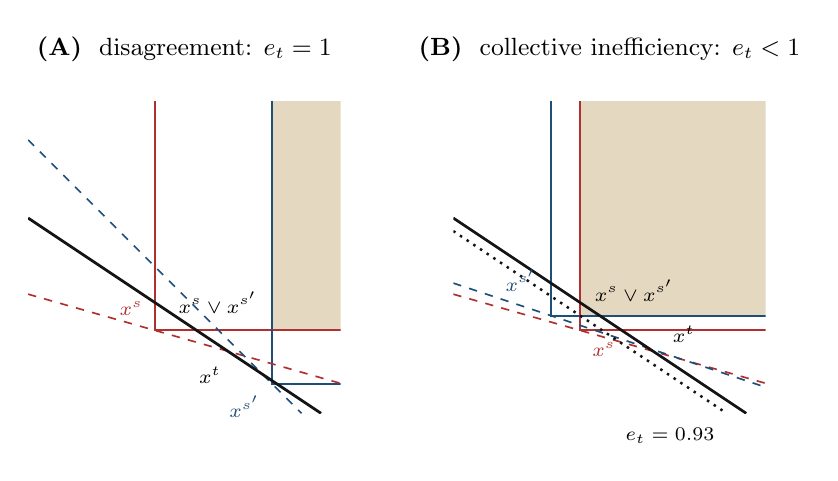
\begin{tikzpicture}[x=0.62cm, y=0.62cm]
%%%%% Panel (A): disagreement, e_t = 1
\begin{scope}
  \begin{scope}
    \clip (0,0) rectangle (6.4,6.4);
    \fill[sand] (5.0,1.7) rectangle (6.4,6.4);
    \draw[memi, line width=.6pt] (2.6,6.4) -- (2.6,1.7) -- (6.4,1.7);
    \draw[memj, line width=.6pt] (5.0,6.4) -- (5.0,0.6) -- (6.4,0.6);
    \draw[memi, dashed, line width=.6pt] (0,2.44) -- (8.55,0);
    \draw[memj, dashed, line width=.6pt] (0,5.6) -- (5.6,0);
    \draw[groupc, line width=1pt] (0,4) -- (6,0);
  \end{scope}
  \ceiframe
  \ceipt{4.2}{1.2}{groupc}
  \ceipt{2.6}{1.7}{memi}
  \ceipt{5.0}{0.6}{memj}
  \ceijoin{5.0}{1.7}
  \node[font=\scriptsize, anchor=north east] at (4.15,1.15) {$x^{t}$};
  \node[font=\scriptsize, anchor=south east, memi] at (2.55,1.8) {$x^{s}$};
  \node[font=\scriptsize, anchor=north east, memj] at (4.95,0.55) {$x^{s'}$};
  \node[font=\scriptsize, anchor=south east] at (4.9,1.85) {$x^{s} \vee x^{s'}$};
  \node[font=\small, anchor=south] at (3.2,7.0) {\textbf{(A)}\ \ disagreement: $e_{t} = 1$};
\end{scope}
%%%%% Panel (B): collective inefficiency, e_t < 1
\begin{scope}[xshift=5.4cm]
  \begin{scope}
    \clip (0,0) rectangle (6.4,6.4);
    \fill[sand] (2.6,2.0) rectangle (6.4,6.4);
    \draw[memi, line width=.6pt] (2.6,6.4) -- (2.6,1.7) -- (6.4,1.7);
    \draw[memj, line width=.6pt] (2.0,6.4) -- (2.0,2.0) -- (6.4,2.0);
    \draw[memi, dashed, line width=.6pt] (0,2.44) -- (8.55,0);
    \draw[memj, dashed, line width=.6pt] (0,2.667) -- (8,0);
    \draw[groupc, line width=1pt] (0,4) -- (6,0);
    \draw[groupc, dotted, line width=.9pt] (0,3.733) -- (5.6,0);
  \end{scope}
  \ceiframe
  \ceipt{4.2}{1.2}{groupc}
  \ceipt{2.6}{1.7}{memi}
  \ceipt{2.0}{2.0}{memj}
  \ceijoin{2.6}{2.0}
  \node[font=\scriptsize, anchor=south west] at (4.3,1.25) {$x^{t}$};
  \node[font=\scriptsize, anchor=north west, memi] at (2.65,1.65) {$x^{s}$};
  \node[font=\scriptsize, anchor=south east, memj] at (1.9,2.3) {$x^{s'}$};
  \node[font=\scriptsize, anchor=south west] at (2.7,2.1) {$x^{s} \vee x^{s'}$};
  \node[font=\scriptsize, anchor=north east] at (5.55,-0.1) {$e_{t} = 0.93$};
  \node[font=\small, anchor=south] at (3.2,7.0) {\textbf{(B)}\ \ collective inefficiency: $e_{t} < 1$};
\end{scope}
\end{tikzpicture}

\begin{minipage}{\textwidth}
\vspace{6pt}
{\footnotesize \emph{Notes}: The dashed diagonal is the certainty line. In both panels the solid black line is the group's budget at collective observation $t$, with $p^{t} = (\tfrac{1}{6}, \tfrac{1}{4})$, and the black dot is the group's choice $x^{t} = (4.2, 1.2)$. The red dot $x^{s}$ is an observation of member $i$ and the blue dot $x^{s'}$ is an observation of member $j$; the dashed red and blue lines are the members' own budgets at those observations, on which $x^{t}$ is affordable, so that $s \in A_{i}(t)$ and $s' \in A_{j}(t)$ by a chain of length zero. The thin red and blue staircases bound the regions that each member's data reveal she would accept in place of $x^{t}$, and the shaded region, the upper orthant with corner at the join $x^{s} \vee x^{s'}$ (open dot), is the region both would accept. In Panel (A), the objectors lie on opposite sides of $x^{t}$: member $i$'s data would move the group's choice toward the certainty line and member $j$'s away from it. Each objection alone closes into a cross violation of $\mathcal{D}^{ig}$ or $\mathcal{D}^{jg}$, which the distance index of \autoref{subsec:rpd} prices, but the join $(5.0, 1.7)$ costs $p^{t} \cdot (x^{s} \vee x^{s'}) = 1.26 > 1$, the shaded region lies outside the budget set, and $e_{t} = 1$. In Panel (B), both objectors lie on the same side of $x^{t}$ and strictly inside the group's budget set; the join $(2.6, 2.0)$ costs $0.93$, so the shaded region reaches inside the budget set. The dotted line is the group's budget contracted to the fraction $e_{t} = 0.93$, the first contraction at which the budget line touches the shaded region: the group could have discarded 7\% of its budget and still afforded a payoff vector that both members' own choices reveal they prefer. No choice in either panel violates first-order stochastic dominance.}
\end{minipage}
\end{figure}

The two panels separate the two objects that this paper measures. In Panel (A), the group's choice lies between the members' objectors, and each member's data would move it in a different direction. This is disagreement: which member's direction the group followed is what the distance index $I_{ig}$ of \autoref{subsec:rpd} measures, and \autoref{lem:objection}(i) shows that each objection contributes to the cross-consistency costs $c_{ig}$ and $c_{jg}$ that enter it. In Panel (B), both members' data would move the group's choice in the same direction, toward the certainty line, and the CEI records how far. On a budget line with two goods, the choices that no affordable alternative Pareto dominates form the interval between the members' most preferred payoff vectors; the CEI flags a choice outside that interval whenever the members' own data reveal it to be so, without estimating their most preferred points.

The following proposition collects the properties of the index and its relation to the measures of \autoref{sec:measurement}.

\begin{proposition}\label{prop:cei}
Fix chain levels $(e_{i}, e_{j}) \in (0,1]^{2}$.
\begin{enumerate}
\item[(i)] If $e_{t} < 1$, then for every pair $(u_{i}, u_{j})$ of continuous and strictly increasing functions such that $u_{m}$ $e_{m}$-rationalizes $\mathcal{D}^{m}$ for each $m \in N$, there is $y \in \mathbb{R}^{2}_{+}$ with $p^{t} \cdot y < 1$ and $u_{m}(y) > u_{m}(x^{t})$ for both $m$. In particular, no such pair provides a collective rationalization of $\mathcal{D}^{g}$ in the sense of \autoref{subsec:two_benchmarks}.
\item[(ii)] If $e_{m} \leq e'_{m}$ for both $m \in N$, then the index at $(e_{i}, e_{j})$ is weakly larger than the index at $(e'_{i}, e'_{j})$. In particular, the untempered index is a lower bound for the index at $(e^{*}_{i}, e^{*}_{j})$.
\item[(iii)] If $\mathcal{D}^{mg}$ admits no cross $e_{m}$-violation for some $m \in N$, then $e^{c}_{g} \geq e_{m}$. In particular, under the untempered specification, $e^{c}_{g} = 1$ whenever no cross $e$-violation of $\mathcal{D}^{Ng}$ at any $e \in (0,1]$ involves member $m$'s dataset, which is the hypothesis under which \autoref{prop:properties}(iii) gives $I_{mg} = 0$.
\end{enumerate}
\end{proposition}

Part (i) is the content of the index: a collective violation certifies a Pareto improvement under \emph{every} pair of utility functions consistent with the members' individual choices at the chain levels, so the CEI tests the collective model of \autoref{subsec:two_benchmarks} against the members' revealed preferences without recovering those preferences. It also identifies where the primary specification matters. If $e^{*}_{m} < 1$, no function $1$-rationalizes $\mathcal{D}^{m}$, the quantifier in part (i) is empty at $e_{m} = 1$, and an untempered violation may reflect nothing more than member $m$'s own inconsistency; at $e_{m} = e^{*}_{m}$ the quantifier is nonempty. Part (ii) orders the two specifications: the untempered index is more demanding and provides an upper bound on the incidence of violations.

Part (iii) states formally that the test requires \emph{both} members to object. A group whose choices never conflict with one member's revealed preferences, the case in which the distance index assigns that member a share of zero and the other member a share of one, is collectively efficient: a dictator's optimum is Pareto efficient. Conversely, a pair can be collectively inefficient only if its choices conflict with both members' datasets, but Panel (A) of \autoref{fig:cei_geometry} shows that such two-sided conflict is not sufficient. A group choice that one member's data reject and the other's accept is a disagreement resolved in the second member's favor, not an inefficiency. The CEI is therefore conservative by design, in that it flags only unambiguous Pareto improvements, and the two measures of this paper read together: $I_{ig}$ locates the group's choices between the members, and $e^{c}_{g}$ asks whether they leave the region both members would accept.

The CEI and the group CCEI $e^{*}_{g}$ of \autoref{subsec:two_benchmarks} are not nested. The following lemma records the two implications that hold and the two that do not.

\begin{lemma}\label{lem:cei_ccei}
Fix chain levels $(e_{i}, e_{j})$.
\begin{enumerate}
\item[(i)] If $\mathcal{D}^{g}$ is generated by maximizing $U_{g}(\cdot\,;b_{i})$ in \eqref{eq:collective_objective} on every budget with $b_{i} \in (0,1)$ fixed, then $e^{*}_{g} = 1$. If in addition $u_{i}$ and $u_{j}$ are continuous and strictly increasing and $u_{m}$ $e_{m}$-rationalizes $\mathcal{D}^{m}$ for each $m$, as is the case when $\mathcal{D}^{i}$ and $\mathcal{D}^{j}$ are generated by maximizing $u_{i}$ and $u_{j}$, then $e^{c}_{g} = 1$.
\item[(ii)] If $\mathcal{D}^{g}$ is generated by maximizing $\mu^{t} u_{i} + u_{j}$ on the budget of each $t$ with $\mu^{t} > 0$ varying across $t$, then $e^{c}_{g} = 1$ under the same condition on the individual datasets, while $e^{*}_{g}$ may be strictly below one.
\item[(iii)] Neither $e^{c}_{g} = 1$ nor $e^{*}_{g} = 1$ implies the other.
\end{enumerate}
\end{lemma}

Part (i) restates the observation made after \eqref{eq:collective_objective} that a stable weight yields unitary consistency, and adds that it also yields collective efficiency. Part (ii) is the case that motivates this section: a pair that alternates between the members' preferred allocations, or otherwise shifts the weight from round to round, is collectively efficient but can violate GARP. Part (iii) states that the two indices are separate measurements. Reading them together decomposes observed inconsistency into interpretable parts. A pair with $e^{*}_{g} < 1$ and $e^{c}_{g} = 1$ is consistent with efficient aggregation under a varying weight; the inconsistency reflects how the pair resolved its disagreement, not a failure to realize gains that both members would recognize. A pair with $e^{c}_{g} < 1$ makes a choice that some affordable alternative dominates under both members' own revealed preferences, which is a failure of decision quality in the strongest sense available without imposing a functional form. Proofs for this subsection are collected in \autoref{appendix:cei}.
\end{comment}
%\paragraph{Power.} Because the test is one-sided, a pair that passes it is not thereby shown to be efficient: with 18 individual observations per member, the objector sets may be too sparse to rule out inefficiency, and the pair's choices may happen to lie in the region the individual data do not discipline.\footnote{This asymmetry is shared by every revealed-preference test; \citet{cherchye2007} make the same point about their sufficiency condition.} We therefore accompany every pass rate with a measure of power following \citet{bronars1987power}: for each pair we keep the members' actual individual choices, replace the collective choices with random points on the actual collective budgets, and recompute the CEI. The gap between the actual index and the distribution of the random index measures the test's ability to detect inefficient behavior for that pair. Because the Pareto set on a budget line is the interval between the members' preferred allocations, power is lower for pairs whose members disagree more; we report power by pair type for this reason.


To begin with, a group of two members with different tastes need not behave like a single decision maker, and a group that consistently aggregates two stable preferences can violate GARP without making any mistake. To distinguish the level of each index from whether it reaches one, \autoref{fig:collective_joint_outcomes} reports the four joint outcomes. XXX explain what each section means, with much more theoretical details XXX Both indices are below one in 415 pair-waves (31.8\%); only CCEI equals one in 117 (9.0\%); only CEIV equals one in 300 (23.0\%); and both equal one in 472 (36.2\%). The two off-diagonal categories illustrate that group consistency and collective rationalizability are distinct benchmarks, as discussed in \autoref{subsec:collective_rationalizability}.

CEIV$<$1, CCEI=1 is not driven by all corner or all midpoint choices. these cases seem to capture that genuinely often times group deliberation shape group choices that are distinct from preferences both individuals bring into the deliberation process. XXX example of detailed figure? XXX 

\begin{figure}[H]
\centering
\singlespacing
\caption{Joint Collective Outcomes}
\label{fig:collective_joint_outcomes}
\includegraphics[width=0.6\textwidth]{figures_2025/collective_rationality/joint_outcome_quadrants.pdf}
\vspace{8pt}
\begin{minipage}{\textwidth}
\footnotesize
\emph{Notes}: The horizontal axis classifies group CCEI and the vertical axis classifies group CEIV. Diagonal cells are blue and off-diagonal cells are white; stripes and dots distinguish outcomes within each color. Each quadrant reports the observed count and percentage of all 1,304 pair-waves from 652 pairs in 64 classes; each pair contributes one observation in each of two waves. These are pooled pair-wave frequencies, rather than a classification of unique pairs. Percentages sum to 100\% before rounding. An index is classified as one at values at least $1-10^{-9}$; all other observations are below one. CEIV endpoint classifications agree with both supplied numerical bounds. The axes represent binary status, rather than distances between continuous index values. CEIV$=1$ denotes rationalizability under the specified individual calibrations and varying weights.
\end{minipage}
\end{figure}

\subsection{Individual Rationality and Collective Outcomes}\label{subsec:cei_results}

We now ask how the rationality of each member relates to two dimensions of collective choice: group CCEI and the varying-weight collective rationalizability index, CEIV, defined in \autoref{subsec:collective_rationalizability}. Group CCEI measures consistency with a single utility function, whereas CEIV measures compatibility with the members' individual choices under the specified individual calibrations and weights that may vary across collective decisions. The analysis pools both waves and uses 1,304 pair-wave observations from 652 pairs in 64 classes. Unlike the revealed-preference-distance regressions in \autoref{tab:pref_agg_ccei}, it retains pairs for which that distance is undefined, since both group indices remain observed.

\autoref{fig:collective_ccei_ceiv_categories} compares group CCEI and CEIV across three pair types. Each member is classified as High if her individual CCEI exceeds the pooled median across both waves (0.9806594), and as Low otherwise. Mean group CCEI rises from 0.877 for Low--Low pairs to 0.928 for Low--High pairs and 0.964 for High--High pairs. Mean CEIV likewise rises from 0.901 to 0.942 and 0.957. All pairwise mean differences are statistically significant in the unadjusted comparisons. The CDF panels show the corresponding full distributions, including the mass at one.

\begin{figure}[h!]
\centering
\caption{Collective CCEI and CEIV by Members' Individual CCEI Category}
\label{fig:collective_ccei_ceiv_categories}
\begin{subfigure}{0.485\textwidth}
\centering
\includegraphics[width=\linewidth]{figures_2025/collective_rationality/group_ccei_bar.pdf}
\caption{Mean collective CCEI}
\end{subfigure}\hfill
\begin{subfigure}{0.485\textwidth}
\centering
\includegraphics[width=\linewidth]{figures_2025/collective_rationality/group_ccei_cdf.pdf}
\caption{CDFs of collective CCEI}
\end{subfigure}
\begin{subfigure}{0.485\textwidth}
\centering
\includegraphics[width=\linewidth]{figures_2025/collective_rationality/group_ceiv_bar.pdf}
\caption{Mean collective CEIV}
\end{subfigure}\hfill
\begin{subfigure}{0.485\textwidth}
\centering
\includegraphics[width=\linewidth]{figures_2025/collective_rationality/group_ceiv_cdf.pdf}
\caption{CDFs of collective CEIV}
\end{subfigure}
\vspace{8pt}
\begin{minipage}{\textwidth}
\footnotesize
\emph{Notes}: Each member is High if individual CCEI exceeds the pooled median across both waves, and Low otherwise; no individual CCEI equals the median. The sample contains 1,304 pair-waves from 652 pairs in 64 classes. Low--Low, Low--High, and High--High contain 348, 608, and 348 pair-waves, respectively. Bars show unadjusted means with 95\% Student-$t$ confidence intervals. Bracket labels are upper-category minus lower-category means; significance uses Welch two-sample $t$-tests. CDFs use all observations, including the mass at one. These descriptive intervals and tests do not adjust for class clustering; \autoref{fig:cei_ame_members} and \autoref{tab:collective_ccei_ceiv_categories} do. +, *, and ** denote $p<0.10$, $p<0.05$, and $p<0.01$.
\end{minipage}
\end{figure}

Appendix \autoref{tab:collective_ccei_ceiv_categories} reports regressions using these categories, with Low--Low as the omitted category. Column (1) includes class fixed effects; Column (2) adds student, friendship, and choice-pattern controls; Column (3) uses these controls with pair fixed effects. Standard errors are clustered by class. The High--High minus Low--High comparison remains significant for group CCEI in all three specifications ($p<0.001$, $p<0.001$, and $p=0.045$), while it is not significant for CEIV ($p=0.111$, $p=0.168$, and $p=0.991$). Thus, the unadjusted increase in CEIV between these two categories is less precisely estimated after accounting for controls and class clustering.

As laid out in  \autoref{fig:collective_joint_outcomes}, CCEI and CEIV jointly define qualities of group choices.  Thus, we examine how individual rationalities define these two outcomes jointly. To this end, for each pair $g$ and wave $t$, let $\text{CCEI}_{\text{max},gt}$ and $\text{CCEI}_{\text{min},gt}$ denote the higher and lower individual CCEIs. We estimate a pooled multinomial logit for the four joint outcomes, with both individual CCEIs entering jointly, the student, friendship, and choice-pattern controls in Column (2) of Appendix \autoref{tab:collective_ccei_ceiv_categories}, and class fixed effects. \autoref{fig:cei_ame_members} reports average marginal effects scaled to a 0.1 increase in the indicated member's CCEI, with class-clustered confidence intervals.

\begin{figure}[h!]
\centering
\singlespacing
\caption{Individual Rationality and Joint Collective Outcomes}
\label{fig:cei_ame_members}
\begin{subfigure}{0.45\textwidth}
\centering
\includegraphics[width=\linewidth]{figures_2025/collective_rationality/figure6_a_ame_maximum.png}
\caption{$\text{CCEI}_{\text{max},gt}$}
\end{subfigure}
\begin{subfigure}{0.45\textwidth}
\centering
\includegraphics[width=\linewidth]{figures_2025/collective_rationality/figure6_a_ame_minimum.png}
\caption{$\text{CCEI}_{\text{min},gt}$}
\end{subfigure}
\vspace{8pt}
\begin{minipage}{\textwidth}
\footnotesize
\emph{Notes}: Pooled four-category multinomial-logit average marginal effects, expressed in percentage points and scaled to a 0.1 increase in the indicated member's individual CCEI. These are scaled average derivatives, rather than exact finite changes in predicted probabilities. Both individual CCEIs enter jointly, with student, friendship, and corner/midpoint share controls and class fixed effects. The control set matches Appendix \autoref{tab:collective_ccei_ceiv_categories}, Column (2); risk-aversion controls and wave fixed effects are excluded. The sample is 1,304 pair-waves from 652 pairs in 64 classes. Horizontal bars are 95\% normal confidence intervals based on class-clustered standard errors. Effects sum to zero across the four outcomes for each member. An index is classified as one within a numerical tolerance of $10^{-9}$. Joint-outcome counts and shares appear in \autoref{fig:collective_joint_outcomes}. CEIV$=1$ denotes rationalizability under the specified individual calibrations and varying weights; it does not identify actual aggregation weights or a communication process. The effects describe conditional associations.
\end{minipage}
\end{figure}


The higher individual CCEI is positively associated with the probability that both group indices equal one. Its average marginal effect, scaled to a 0.1 increase, is 19.2 percentage points, compared with 2.4 percentage points for the lower individual CCEI; both 95\% confidence intervals exclude zero. The lower individual CCEI also has a positive effect of 2.5 percentage points on the outcome with CCEI$=1$ and CEIV$<1$. These estimates describe conditional associations with category probabilities, rather than observed transitions of particular pairs, and the figure does not test equality of the two members' effects.


XXX the role of other variables: how do other covariates' AME figures look like? Shapley decomposition? also robustness using other rationality measures, but only show the variation of figure 8 XXX


Together, these results connect individual rationality to both group consistency and compatibility with the members' individual choices. They complement the finding in \autoref{tab:pref_agg_ccei} that collective choices are more closely aligned with those of the more rational member. CEIV permits weights to vary, including the special case of constant weights, so neither the joint outcomes nor the marginal effects identify actual aggregation weights or the process through which pairs reach agreement.

%%%%%%%%%%
\section{Mechanism}

\subsection{A Framework of Rationality-Weighted Deliberation}
\label{sec:framework}

We provide a parsimonious framework to organize the relationship between individual rationality, deliberation, and preference aggregation. Its central distinction is between a member's underlying preferences and the precision with which she implements those preferences. Members may disagree in tastes without either preference being normatively superior, while differing in how consistently their choices reveal a stable preference.

Consider a pair $g$ with members $i$ and $j$. Member $k\in\{i,j\}$ has a stable utility function $u_k$ over the two Arrow securities and a latent decision precision $r_k>0$. One way to make this interpretation concrete is a random-utility representation. On individual budget $B_{kt}$, member $k$ chooses
\begin{equation}
    x_{kt}\in\arg\max_{x\in B_{kt}}
    \left\{u_k(x)+r_k^{-1/2}\varepsilon_{kt}(x)\right\},
    \label{eq:random_utility_appendix}
\end{equation}
where $\varepsilon_{kt}(x)$ is a mean-zero choice disturbance. This decision problem distinguish tastes, represented by $u_k$, from the precision with which those tastes are implemented.

Let $R_k$ denote the observed CCEI. We assume only
\begin{equation}
    \mathbb{E}[R_k\mid r_k]=m(r_k),
    \qquad m'(r_k)>0.
    \label{eq:ccei_precision_appendix}
\end{equation}
The CCEI is therefore interpreted as a monotone proxy for latent decision precision, rather than as a cardinal measure of $r_k$. 

Deliberation determines how effectively differences in decision precision translate into collective choice. We distinguish a member-specific component from the common deliberative environment. Let $d_{kg}$ denote member $k$'s deliberative effectiveness: her ability to formulate and communicate a recommendation in a way that can be understood and assessed by her partner. Let $q_g$ denote the quality of the deliberative environment: features of the pair or classroom that facilitate substantive exchange and the evaluation of competing recommendations.

In our data, mathematics performance and in-degree in the classroom friendship network are plausible correlates of member-specific deliberative effectiveness, $d_{kg}$. Greater cognitive ability may help a member formulate, compare, and articulate the arguments underlying her preferred allocation, whereas greater in-degree may make her recommendations more salient, credible, or readily received by her partner. By contrast, the second wave and a classroom with fewer socially excluded students are plausible correlates of the common deliberative environment, $q_g$. The same pairs remain together across waves separated by approximately four months, so later interaction may facilitate mutual understanding during deliberation. Similarly, a classroom with fewer socially excluded students may reflect a more socially inclusive setting in which communication and the assessment of competing recommendations face fewer frictions.

Suppose that communication introduces a common noise variance $\tau^2(q_g)$, where $\tau^{2\prime}(q_g)<0$. The effective precision with which member $k$'s underlying preference is conveyed is
\begin{equation}
    \pi_k(q_g)=\left(r_k^{-1}+\tau^2(q_g)\right)^{-1}
    =\frac{r_k}{1+r_k\tau^2(q_g)}.
    \label{eq:effective_precision}
\end{equation}
Let $a(d_{kg})>0$, with $a'(d)>0$, capture the member-specific effectiveness with which this recommendation enters deliberation. We summarize the resulting deliberative weight by
\begin{equation}
    b_{kg}=\frac{a(d_{kg})\pi_k(q_g)}{a(d_{ig})\pi_i(q_g)+a(d_{jg})\pi_j(q_g)},
    \qquad b_{ig}+b_{jg}=1.
    \label{eq:deliberative_weight}
\end{equation}
The weight $b_{kg}$ is a latent theoretical object, not the revealed-preference distance measured in the data.

Let $H$ and $L$ denote the higher- and lower-precision members, with $r_H>r_L$. The framework yields three directly interpretable implications.

\begin{proposition}
\label{prop:deliberation}
Suppose $r_H>r_L$ and $a'(d)>0$.
\begin{enumerate}
    \item Holding deliberative effectiveness and the common environment fixed, greater decision precision raises a member's deliberative weight. In particular, if $d_{Hg}=d_{Lg}$, then $b_{Hg}>b_{Lg}$.
    \item Holding decision precision and the common environment fixed, greater deliberative effectiveness raises a member's deliberative weight.
    \item The relative deliberative-weight advantage associated with greater decision precision is larger in a better deliberative environment---that is, when communication noise is lower.
\end{enumerate}
\end{proposition}

The first implication is the framework's basic rationality-weighting result: when two members are equally able to communicate their views, the member whose choices more reliably implement a stable preference receives greater deliberative weight. The second allows this relationship to be amplified or attenuated by a member's ability to make her recommendation effective in discussion. Cognitive ability may facilitate the formulation and evaluation of a coherent argument, while social connectedness may affect whether a recommendation receives attention or is treated as credible.

The third implication is a communication-complementarity result. When communication is noisy, both members' recommendations are blurred by a common source of error, compressing the difference between a more and a less precise decision maker. As the deliberative environment improves, this common noise recedes and underlying differences in decision precision become more consequential. Formally,
\begin{equation}
    \log\frac{b_{Hg}}{b_{Lg}}=
    \log\frac{a(d_{Hg})}{a(d_{Lg})}+
    \log\frac{r_H}{r_L}+
    \log\frac{1+r_L\tau^2(q_g)}{1+r_H\tau^2(q_g)}.
    \label{eq:log_weight}
\end{equation}
The final term shows why better communication strengthens the role of relative decision precision. This mechanism is consistent with work emphasizing persuasive arguments, preference consistency, and information exchange in group deliberation \citep{burnstein1975what,goeree2011experimental,mojzisch2014consistency}.

The empirical analysis does not observe $b_{kg}$. It observes the revealed-preference distance $I_{kg}$, with lower values indicating that collective choices are closer to member $k$'s individually revealed preferences. We therefore impose only the monotone interpretation
\begin{equation}
    \mathbb{E}[1-I_{kg}\mid b_{kg},Z_g]=h(b_{kg},Z_g),
    \qquad \frac{\partial h}{\partial b}>0,
    \label{eq:distance_mapping}
\end{equation}
where $Z_g$ collects features of the realized choice environment. A lower revealed-preference distance does not by itself establish that a member actively persuaded her partner; rather, it means that collective choices are more closely aligned with that member's revealed preferences.

The framework therefore gives a direct interpretation to the heterogeneity analysis in Section~6.2. A stronger rationality--distance relationship when the more rational member has a higher mathematics score or greater in-degree is consistent with greater member-specific deliberative effectiveness. Its strengthening in the second wave and in classrooms with fewer socially excluded students is consistent with a deliberative environment in which recommendations can be communicated and assessed more effectively. Because these moderators are not experimentally assigned, we interpret these patterns as evidence on the conditions under which rationality-based preference aggregation is most pronounced, rather than as causal effects of the moderators themselves.

The framework can also organize the relationship between members' decision precision and the internal consistency of collective choices. As a benchmark, suppose that the pair uses a stable deliberative weight $b_{ig}=b_i$ and therefore has the collective objective
\begin{equation}
    U_g(x;b_i)=b_i u_i(x)+(1-b_i)u_j(x).
    \label{eq:collective_objective}
\end{equation}
If the pair maximized equation~\eqref{eq:collective_objective} exactly on every budget, the resulting choices would be rationalizable by a single utility function. Unequal deliberative weights by themselves therefore need not generate revealed-preference inconsistency.

Collective choices may nevertheless be implemented imperfectly. We summarize the precision of the collective decision process by total effective precision,
\begin{equation}
    \Pi_g=\pi_i(q_g)+\pi_j(q_g),
    \label{eq:collective_precision_appendix}
\end{equation}
and represent collective choice as
\begin{equation}
    x_{gt}\in\arg\max_{x\in B_{gt}}\left\{U_g(x;b_i)+\Pi_g^{-1/2}\varepsilon_{gt}(x)\right\}.
    \label{eq:collective_random_utility}
\end{equation}
Because the CCEI is a nonlinear statistic of a finite set of choices, we do not impose an exact analytical mapping from $\Pi_g$ to collective CCEI. Instead, let $R_g$ denote collective CCEI and assume
\begin{equation}
    \mathbb{E}[R_g\mid\Pi_g]=G(\Pi_g), \qquad G'(\Pi_g)>0.
    \label{eq:collective_ccei_mapping}
\end{equation}

\begin{proposition}
\label{prop:collective_precision}
Suppose that expected collective CCEI is increasing in $\Pi_g$ and that communication noise is positive.
\begin{enumerate}
    \item An increase in either member's decision precision raises expected collective CCEI.
    \item The marginal contribution of an increase in decision precision is larger for the less precise member.
\end{enumerate}
\end{proposition}

This result is important because rationality-weighted deliberation does not imply that the less rational member is irrelevant. Collective choices may be tilted toward the more precise member's revealed preferences, but both members supply effective precision to the joint decision. Moreover, effective precision exhibits diminishing returns: improving an already highly precise recommendation matters, but an equal improvement in the less precise recommendation can matter more. This is the theoretical counterpart to the empirical result in Section~7 that both members' CCEIs positively predict collective CCEI, with the coefficient on the lower-CCEI member larger. Proofs and further details are provided in Appendix~D.


\subsection{What Mediate Individual Rationality's Effect on Group Choices?}
\label{sec:heterogeneity}

Having established that collective choices are systematically closer to the individual choices of more rational members, we next examine when this rationality--distance relationship is stronger. One possible mechanism is that greater rationality is associated with more consistent and clearly defined preferences, which may be easier to articulate during deliberation. Under this interpretation, the revealed-preference distance of the more rational member should be especially low when communication within the pair is easier or when she can convey her preferences more effectively. This prediction is consistent with evidence that communication plays an important role in group deliberation \citep[e.g.,][]{burnstein1975what, goeree2011experimental}.

% TODO: Current Ihat_ig/HighCCEI_both_high GATES outputs are missing; archived estimates use different definitions.
Following \citet{chernozhukov2018generic}, we conduct a data-driven Classification Analysis (CLAN) to examine heterogeneity in the extent to which group choices align with the more rational member's individual choices. We train several machine-learning algorithms to rank observations by this predicted alignment. We prespecify five quintiles of the ranking and compare observable characteristics in the two extremes: the 20\% of observations in which group choices are predicted to be most closely aligned with the more rational member's individual choices and the 20\% in which they are predicted to be least closely aligned. We find significant heterogeneity: the average estimated difference in revealed-preference distance between higher- and lower-CCEI members is XXX in the most-aligned quintile and XXX in the least-aligned quintile (Appendix Figure XXX; Appendix Table XXX). \autoref{fig:clan_selected_boosting} presents selected results from the boosting specification, while \autoref{tab:clan_clb_rf} and \autoref{tab:clan_clb_rf2} report the full CLAN results.

%\autoref{fig:mechanism_heterogeneity} presents the Higher CCEI coefficient estimated separately on subgroups defined by pair characteristics. Panel (a) splits pairs by mutual friendship and observable traits such as gender composition. In each case, the coefficient is more negative for the subgroup likely to communicate more easily (mutual friends, same sex), but these differences are not statistically significant. This null result is itself informative: it reaffirms that the rationality advantage does not operate primarily through demographic or social channels, complementing the regression evidence in \autoref{tab:pref_agg_ccei} that observable controls leave the effect intact.

%We next examine which observable characteristics distinguish settings in which the more rational member exerts a larger influence on the group decision. Demographic and cognitive characteristics provide relatively little robust evidence. The Boosting estimates suggest that the rationality premium is larger when the more rational member has a lower math score and is less outgoing relative to the partner, but these patterns do not persist under Random Forest. Gender composition is likewise not robustly associated with the estimated premium. Among personality traits, lower agreeableness is the only consistent predictor across the two algorithms.
%In contrast, the friendship-network results reveal a clear pattern. The rationality premium is larger when the focal individual has more friends, is more popular among classmates, and shares a mutual friendship with the partner. The within-pair differences in network measures are generally insignificant, suggesting that absolute social embeddedness and relational closeness matter more than a network advantage over the partner.
%The broader classroom environment also matters. The rationality premium is larger at endline and among students who report less social exclusion and greater fairness among their peers. We also find a robust association with the horizontal-PBL measure, although its direction requires careful interpretation based on the survey scale. By contrast, teacher induction and most other measures of classroom climate are not systematically related to the estimated premium.
%Taken together, the most consistent results concern the social setting in which deliberation occurs. Rationality translates more strongly into influence when the individual is socially embedded, when the pair shares a mutual relationship, and when the classroom environment is less exclusionary. These findings are consistent with communication facilitating the translation of decision-making quality into bargaining influence.


\begin{figure}[H]
\centering
\caption{Predictors of Alignment with the More Rational Member}
\label{fig:clan_selected_boosting}
\begin{subfigure}[b]{0.5\textwidth}
  \centering
  \includegraphics[width=\textwidth]{figures_2025/Figure_clan_selected_boosting_demographics.pdf}
  \caption{Demographics and Skills}
\end{subfigure}
\begin{subfigure}[b]{0.5\textwidth}
  \centering
  \includegraphics[width=\textwidth]{figures_2025/Figure_clan_selected_boosting_network.pdf}
  \caption{Friendship Network}
\end{subfigure}
\begin{subfigure}[b]{0.5\textwidth}
  \centering
  \includegraphics[width=\textwidth]{figures_2025/Figure_clan_selected_boosting_classroom.pdf}
  \caption{Classroom Environment}
\end{subfigure}
\vspace{12pt}
\begin{minipage}{\textwidth}
 {\footnotesize \emph{Notes}: The figure reports selected results from the boosting specification of the Classification Analysis. The machine-learning model estimates how the effect of higher individual rationality on revealed preference distance varies across observations. We partition the estimated heterogeneity score into five quantile groups and compare the two extreme groups, corresponding to the bottom and top 20 percent of the score distribution. For each characteristic, points show the difference between its mean in the group with the less negative estimated coefficient on higher CCEI and its mean in the group with the more negative coefficient, divided by the full-sample standard deviation of that characteristic. Negative values indicate that larger values of the characteristic are associated with a smaller revealed preference distance index for the more rational individual, meaning that collective choices align more closely with the more rational individual's choices. Horizontal bars show 95\% confidence intervals. Blue triangles indicate differences with adjusted $p<0.05$; open circles indicate otherwise.}
\end{minipage}
\end{figure}

\autoref{fig:clan_selected_boosting} compares observable characteristics between the most- and least-aligned quintiles in the boosting specification. The most-aligned quintile is characterized by a higher math score and greater in-degree for the more rational member, suggesting that cognitive ability and popularity within the friendship network help her steer group choices toward her individual choices. Group choices are also more closely aligned with the more rational member's choices in the second wave and in classrooms with fewer socially excluded students. These patterns are consistent with the interpretation that repeated interaction and a more inclusive classroom environment facilitate communication during deliberation. Mutual friendship points in the same direction, although the difference is not statistically significant. Other demographic, friendship-network, and classroom characteristics—including gender composition, outgoingness, and encouragement of participation—do not differ significantly between the two extreme quintiles.

\begin{comment}

\begin{figure}[H]
\small
\centering
\caption{Heterogeneity Analysis}
\label{fig:mechanism_heterogeneity}
\subfigure[Panel (a): Mutual friendship, observable characteristics]{%
  \centering
  \includegraphics[width=0.48\textwidth]{figures_2025/fig6_A_ver1}
}
\subfigure[Panel (b): PBL related]{%
  \centering
  \includegraphics[width=0.48\textwidth]{figures_2025/fig6_B_ver1}
}
\vspace{1em}
\subfigure[Panel (c): Class participation without mentioning PBL]{%
  \centering
  \includegraphics[width=0.48\textwidth]{figures_2025/fig6_C_ver1}
}
\vspace{6pt}
\begin{minipage}{0.9 \textwidth}
{\footnotesize \emph{Notes}: 
This figure illustrates the heterogeneity of the HighCCEI coefficients. Confidence intervals are at the 95\% level. We tested whether the two coefficients for each pair are statistically different. \textit{Value Trust} and \textit{PBL Share Idea} were found to be significantly different, highlighted with a red diamond, and the corresponding $p$-values are displayed below the lines. Statistical significance of the coefficients is denoted by ** $p<0.05$ and *** $p<0.01$.}
\end{minipage}
\end{figure}

Panels (b) and (c) uncover significant heterogeneity along dimensions that more directly capture the substance of in-class interaction. In Panel (b), which exploits items related to project-based learning (PBL), the bargaining advantage of the more rational member is significantly larger in pairs where both members come from classrooms with frequent idea sharing (PBL Share Idea). In Panel (c), which uses non-PBL measures of class participation, the advantage is significantly larger when both members report that they value trust (Value Trust). These two patterns are consistent with the persuasive-arguments mechanism of \citet{burnstein1975what}: more rational members exert greater influence in environments where substantive idea exchange is easier and more credible. The contrast with the null result on observable demographics in Panel (a) suggests that the channel operates through how individuals deliberate rather than through who they are.
\end{comment}

\begin{comment}
\subsection{Procedural Heuristics: Taking Turns?}
One plausible alternative mechanism concerns the procedure through which pairs reach collective choices. Rather than deliberating toward a stable compromise or consistently following one member’s recommendation, the two members may take turns controlling the collective decision. Under this procedure, the more rational member may simply make more internally consistent choices during her turns. The resulting collective dataset could then be more compatible with her individual choices even without the more rational member persuading her partner or the pair converging toward her preferences. Such a procedural heuristics would not contradict our main finding that collective choices are closer to the more rational member, but it would provide a different interpretation from the communication-based mechanism considered above.

To examine this possibility, we exploit the sequential structure of the collective-choice task. Holding fixed all 18 individual choices of each member, we calculate revealed-preference distance separately using the odd-numbered and even-numbered collective rounds. For exposition, we select the member with the lower distance in the full collective-choice dataset and keep that member fixed throughout the exercise. For each pair-wave $gt$, we define the observed split gap as $T^{obs}_{gt}=\lvert\widehat I^{odd}_{igt}-\widehat I^{even}_{igt}\rvert$. Because the two members’ indices are complementary within each partition, this absolute difference is identical for both members and can be interpreted as a pair-wave-level measure. If taking-turns is a common procedure adopted by pairs, then one can expect the gap to be large. To benchmark the magnitude of this measure, we conduct a permutation test where we repeatedly assign the 18 collective choices to two randomly selected sets of nine and recalculating the corresponding split gap by 500 times. This procedure captures the divergence that arises mechanically from estimating the index on smaller subsets of collective choices.\footnote{This procedure also captures other pair-wave-level factors that decides the magnitude of this measure. For example, the index can be mechanically small if two members share similar preferences. By comparing the distribution of $T^{obs}_{gt}$ and index from the permutation test, we examine if the distribution of the former seems to be compatible with taking-turns holding such pair-wave-level factors constant. }

Figure \ref{fig:taking_turns_cdf} compares the CDF of the observed odd–even gaps with the corresponding distribution generated by randomly halving the collective choices. Panel (a) reports the comparison for all pair-waves, while Panel (b) focuses on pairs in the bottom quartile of the overall within-pair distance gap, for which procedural alternation may be particularly relevant given that it will result in similar distance measure between the two members. In both panels, the observed and placebo distributions overlap closely. The observed mean and median gaps are 0.228 and 0.147, compared with placebo values of 0.221 and 0.150, and the distribution of two CDFs are not different from each other ($p=$ 0.839 (median), 0.517 (median) in Panel (a) and (b), respectively). 

We next examine whether the small number of pair-waves displaying unusually large odd–even divergence accounts for our principal result. We classify a pair-wave as turn-like when its observed split gap exceeds the 95th percentile of its pair-wave-specific placebo distribution, exclude both member observations from these pair-waves, and re-estimate the specifications from Section \ref{sec:main_results}. As shown in Table \ref{tab:taking_turns_exclusion}, the coefficient on the higher-CCEI-member indicator remains negative, statistically significant, and similar in magnitude to the full-sample estimate. The coefficient changes from -0.293 in the original specification to -0.289 after the exclusion, and the difference between the two estimates is not statistically significant ($p=$ 0.455). The relationship between individual rationality and revealed-preference distance therefore does not appear to be driven by the pair-waves for which we detect unusually strong temporal alternation.

Taken together, these results provide little evidence that systematic odd–even taking turns is a common collective-choice procedure in our sample. This conclusion does not rule out isolated instances of taking turns, alternation that does not follow odd–even parity\footnote{To examine this possibility, we conducted the same exercise where we split group choices into the first half rounds and the second half rounds. Results are presented in appndix Figures \ref{fig:taking_turns_first_last} and \ref{fig:taking_turns_first_last_ks} and remain the same as the one discussed above.}, or procedures that cannot be detected precisely using nine collective choices per partition. Nevertheless, the close correspondence between the observed and placebo distributions, together with the stability of the main estimates after excluding turn-like pair-waves, suggests that procedural alternation does not explain our central result. More broadly, the exercise illustrates how our revealed-preference framework can be extended to subsets of collective choices to study not only whose preferences collective decisions resemble, but also the behavioral procedures through which preferences are aggregated.

\textcolor{red}{To conclude the section, we visit another alternative behavioral procedure: being assigned to move seats for the collective-choice rounds might affect whose individual preference is more reflected in group choices. Appendix \autoref{tab:bargaining_ccei_ihat_mover} shows that mover status is not statistically associated with revealed-preference distance, nor does mover status significantly moderate the relationship between higher-CCEI status and revealed-preference distance (see the interaction coefficients in Columns~(1)--(3)).}

%%%%%%%%%%
\section{From Individual to Group Rationality}
\label{sec:rationality_extension}

The results in \autoref{section:results} show that group choices are more closely aligned with those of the more rational member. This pattern suggests a channel through which individual decision-making quality of the more rational one may shape the rationality of group choices. At the same time, the coefficient on Higher CCEI in \autoref{tab:pref_agg_ccei} is smaller than $-1$, indicating that the less rational member's choices also remain reflected in the group decision. Thus, the rationality of both members may be relevant for collective rationality.

\autoref{fig:cdf_ccei_g} provides evidence consistent with this prediction. We classify each member as High if her individual CCEI exceeds the pooled sample median and as Low otherwise. Panel (a) reports mean group CCEI across the resulting pair types: Low--Low, Low--High, and High--High. Mean group CCEI rises monotonically from 0.877 for Low--Low pairs to 0.928 for Low--High pairs and 0.964 for High--High pairs. The difference between High--High and Low--Low pairs is 0.087, or 64.5\% of the standard deviation of group CCEI (\autoref{tab:ccei_summary}). All three pairwise mean differences are statistically significant at the 1\% level. Panel (b) further shows that the distributions of group CCEI differ across all three pair types (pairwise Kolmogorov--Smirnov tests: $p<0.01$). Given the random assignment of partners within classrooms, these patterns support a causal interpretation: groups composed of more rational members make more rational collective choices.


\begin{figure}[H]
\small
\caption{Collective CCEI By Members' Individual CCEI Category}
\label{fig:cdf_ccei_g}
\centering
\begin{subfigure}{0.485\textwidth}
    \centering
  \includegraphics[width=\textwidth]{figures_2025/group_ccei_by_member_ccei_median_bar.png}
  \caption{Mean Collective CCEI}
\end{subfigure}
\begin{subfigure}{0.485\textwidth}
    \centering
  \includegraphics[width=\textwidth]{figures_2025/group_ccei_by_member_ccei_median_cdf.png}
  \caption{CDFs of Collective CCEI}
\end{subfigure}
\vspace{12pt}
\begin{minipage}{\textwidth}
{\footnotesize \emph{Notes}: Panel (a) reports mean collective CCEI ($ccei_g$) with 95\% confidence intervals for three pair categories,  Low--Low, Low--High, and High--High, where we classify each member as High if her individual CCEI exceeds the pooled sample median and as Low otherwise. Panel (b) reports the corresponding empirical CDFs. Difference labels in Panel (a) report two-sample $t$-tests; +, *, and ** denote $p<0.10$, $p<0.05$, and $p<0.01$, respectively.}
\end{minipage}
\end{figure}


\autoref{tab:collective_ccei} reports the estimates. Column (1) includes the two CCEI variables and class fixed effects. The coefficient on $\text{CCEI}_{\text{max}}$ is 0.362 ($p<0.01$): a one-standard-deviation increase in the more rational member's CCEI is associated with a 0.156-standard-deviation increase in group CCEI. The coefficient on $\text{CCEI}_{\text{dist}}$ is -0.234 ($p<0.01$). Conditional on $\text{CCEI}_{\text{max}}$, a one-standard-deviation increase in the within-pair CCEI gap is associated with a 0.232-standard-deviation decrease in group CCEI.\footnote{The standard deviations of group CCEI, the CCEI of the more rational member, and the CCEI of the less rational member are 0.1345, 0.058, and 0.128, respectively. Thus, for example, 0.156-standard-deviation comes from $0.262\times\frac{0.058}{0.1345}$. }

\begin{table}[H]
\centering
\caption{Collective CCEI}
\label{tab:collective_ccei}
\begin{tabular}{lcccc}
\toprule \hline
Dependent variable: $CCEI_g$ & (1) & (2) & (3) & (4) \\
\midrule
\input{tables_2025/final_collective_ccei_high_low}
\end{tabular}

\begin{minipage}{\textwidth}
{\footnotesize \emph{Notes}: $CCEI_{high}$ and $CCEI_{low}$ denote the higher and lower individual CCEIs within each pair in each wave, respectively. Columns (1)--(3) are pooled OLS specifications with class fixed effects. Column (4) includes pair fixed effects. Standard errors are clustered at the class level and reported in parentheses. Student controls include gender composition, height, math scores, and Big Five personality traits, as well as missing indicators. Friendship controls include the number of friends, popularity within the class, and whether two students within a pair identified each other as friends. RA controls include the maximum and absolute within-pair difference of the two members' risk-aversion measures. Corner and midpoint share controls include the maximum and absolute within-pair difference of the two members' shares of individual choices made exactly at a corner or at the 50/50 allocation, respectively. +, *, and ** denote significance at the 10\%, 5\%, and 1\% levels, respectively.}
\end{minipage}
\end{table}
\end{comment}


\begin{comment}
    
\begin{table}[H]
\centering
\caption{Collective CCEI}
\label{tab:collective_ccei}
\begin{tabular}{lcccc}
\toprule \hline
Dependent variable: $CCEI_g$ & (1) & (2) & (3) & (4) \\ \midrule
\input{tables_2025/final_collective_ccei}
\end{tabular}
\begin{minipage}{\textwidth}
{\footnotesize \emph{Notes}: Columns (1)--(3) are pooled OLS specifications with class fixed effects. Column (4) includes pair fixed effects. Robust standard errors are clustered at the class level. Student controls include gender composition, height, math scores, and Big Five personality traits, as well as missing indicators. Friendship controls include the number of friends, popularity within the class, and whether two students within a pair identified each other as friends. RA controls include the maximum and absolute within-pair difference of the two members' risk-aversion measures. Corner and midpoint share controls include the maximum and absolute within-pair difference of the two members' shares of individual choices made exactly at a corner or at the 50/50 allocation, respectively. +, *, and ** denote significance at the 10\%, 5\%, and 1\% levels, respectively.}
\end{minipage}
\end{table}

\end{comment}

The pattern remains stable as controls are added. Column (2) adds student and friendship characteristics, and Column (3) further controls for the members' risk-aversion measures and their shares of choices at corners and midpoints of the budget lines. These controls leave the coefficients on $CCEI_{max}$ and $CCEI_{dist}$ largely unchanged. Column (4) replaces class fixed effects with pair fixed effects. Although both coefficients decline in magnitude, they remain statistically and economically significant. The pair-fixed-effects estimates show that, within the same pair, changes in members' CCEIs are systematically related to changes in group CCEI after absorbing stable pair characteristics, including time-invariant compatibility. These estimates indicate that group rationality rises with the CCEI of the more rational member and falls with the within-pair CCEI gap. In sum, the results in \autoref{tab:collective_ccei} show that individual rationality—rather than its observed correlates or stable unobserved pair characteristics—is a key determinant of whether group choices are consistent with utility maximization. The Shorrocks--Shapley decomposition of the $R^2$ from Column (4), reported in \autoref{fig:shapley_groupccei}, attributes 37.4\% of the explained variation in group CCEI to the individual-CCEI block, further underscoring the importance of directly measuring individual rationality. The full specification is reported in \autoref{tab:collective_ccei2}. Appendix Tables \autoref{tab:collective_fgarp} and \autoref{tab:collective_rev_max_mpi} report analogous results using alternative rationality measures and confirm that the results remain similar.

%%%%%%%


\section{Conclusion}\label{section:conclusion}

In this paper, we study how individual rationality shapes group decision-making, using a large-scale panel experiment in which 1,304 Korean middle-school students were randomly assigned into pairs. Our central methodological contribution is a nonparametric revealed-preference distance that builds on the CCEI and applies to all subjects, including those whose choices violate utility maximization. We find that collective choices are substantially closer to the choices of the more rational member. Group rationality itself rises with the more rational member's CCEI and falls with the within-pair gap, while observable demographic and social traits play only a limited role. The alignment between collective choices and the more rational member's choices is especially pronounced in environments that facilitate substantive idea exchange, consistent with a persuasive-arguments interpretation of the rationality--distance relationship.

Methodologically, the revealed-preference distance extends the analysis of preference aggregation to populations whose choices violate the parametric structure required by standard approaches, including children, the elderly, and others who have so far been largely excluded from collective-choice experiments. Substantively, the result that rationality, rather than demographics, friendship, or cognitive ability, is the strongest predictor of whose choices are more closely reflected within a pair suggests that interventions which improve individual decision quality may improve the quality of group decisions.

Several questions remain open. The aggregate index is silent on whether pairs whose members have equal revealed-preference distances are using stable compromise rules or procedural alternation, and round-level analysis is needed to distinguish these. Extending the framework to groups with more than two members, and to settings in which preferences differ along dimensions beyond risk, are natural next steps to explore.

%%%%%%%%%%%%%%%%%%%%%%%%%%%%%%%%%%%%%%%%%%%%%%%%%%%%%%%

\newpage

\printbibliography

%%%%%%%%%%%%%%%%%%%%%%%%%%%%%%%%%%%%%%%%%%%%%%%%%%%%%%%

\clearpage

\appendix
\pagenumbering{arabic}

\doublespacing
%\onehalfspacing

\counterwithin{equation}{section} % Restart equation numbering in each appendix section
\renewcommand{\theequation}{\thesection.\arabic{equation}}

%\renewcommand{\theequation}{(\thesection.\arabic{equation})} % Add parentheses around the numbers

%%%%%%%%%%%%%%%%%%%%%%%%%%%%%%%%%%%%%%%%%%%%%%%%%%%%%%%
\setcounter{figure}{0}
\renewcommand{\thefigure}{A\arabic{figure}}

\setcounter{table}{0}
\renewcommand{\thetable}{A\arabic{table}}

\setcounter{theorem}{0}
\renewcommand{\thetheorem}{A\arabic{theorem}}

\setcounter{proposition}{0}
\renewcommand{\theproposition}{A\arabic{proposition}}

\setcounter{lemma}{0}
\renewcommand{\thelemma}{A\arabic{lemma}}

%%%%%%%%%%%%%%%%%%%%%%%%%%%%%%%%%%%%%%%%%%%%%%%%%%%%%%%

\section{Additional Figures}\label{appendix:figures}
\begin{figure}[H]
\centering
\caption{Photograph From The Fieldwork}\label{fig:photoshoot}
\includegraphics[width=0.7\textwidth]{figures_2025/pblrealshot.jpeg}
\vspace{12pt}
\begin{minipage}{\textwidth}
{\footnotesize \emph{Notes}: This photo was taken from the fieldwork. We rented laptops and set them up in participating classrooms. All sessions were computerized through oTree \citep{Chenetal:2015:JBEF} on these laptops connected to a classroom Wi-Fi router. Four trained experimenters concurrently conducted sessions across participating classes in a school.}
\end{minipage}
\end{figure}

\begin{figure}[H]
\centering
\caption{Illustration Of The Experimental Design }\label{fig:decition_problem_example}
\begin{tikzpicture}[scale = 0.80]
% axes
\draw[->, thick] (0,0) -- (7,0) node[anchor = west] {$x_r$};
\draw[->, thick] (0,0) -- (0,7) node[anchor = east] {$x_b$};
% 45 degree line
\draw[thick, dashed] (0,0) -- (6,6);
\draw (6, 6) node[anchor = south] {$x_b = x_r$};
% budget lines
\draw[thick] (6,0) -- (0,4);
% prices
%\draw[->, thick] (6,0) -- (6+1/2, 1) node[anchor = south] {$p = (p_r, p_b)$};
% bundles
\draw (2.4, 2.4) node {\textbullet};
\draw (2.4, 2.4) node[anchor = north] {$A$};
\draw (4, 4-2/3*4) node {\textbullet};
\draw (4, 4-2/3*4) node[anchor = north] {$C$};
\draw (6, 0) node {\textbullet};
\draw (6, 0) node[anchor = south] {$B$};
\end{tikzpicture}
\begin{minipage}{\textwidth}
{\footnotesize \emph{Notes}: This figure illustrates the decision environment faced by the subjects. The horizontal axis represents the values of $x_r$, and the vertical axis denotes the values of $x_b$. Points $A$, $B$, and $C$ represent possible portfolio choices on a common linear budget set corresponding to a given price pair $(p_r, p_b)$ with $p_r < p_b$. Portfolio $A$ lies on the $45^\circ$ line (dashed), yielding a constant return regardless of the realized state. Portfolio $B$ corresponds to the case where all wealth is allocated to the cheaper security associated with state $r$. Portfolio $C$ represents an intermediate allocation between $A$ and $B$. The figure also illustrates the risk-aversion measure $ra^k$ introduced in \autoref{subsec:risk_aversion}. Since $p_r < p_b$, $x_b$ is the more expensive asset and $ra^k = x_b^k / (x_r^k + x_b^k)$ for any choice $x^k$ on this budget. Portfolio $A$ on the $45^\circ$ line yields $ra^A = 1/2$, the maximum value of the measure, reflecting extreme risk aversion. Portfolio $B$ at the corner where all wealth is on the cheaper asset yields $ra^B = 0$, the minimum, reflecting risk neutrality or risk seeking. Portfolio $C$ lies between the two and yields $ra^C = 1/4$. The measure thus takes values in $[0, 1/2]$, with larger values indicating greater risk aversion.

Because the two states are equally likely, a choice with $ra^k > 1/2$ is first-order stochastically dominated by any choice on the same budget with $ra^k < 1/2$. In our data, 22.89\% of individual decisions (6,477 out of 28,294) and 21.12\% of group decisions (2,988 out of 14,148) fall in this dominated region; relaxing the cutoff to $0.6$ to allow for trembling around the $45^\circ$ line reduces these counts to 2,276 and 812, respectively.}
\end{minipage}
\end{figure}

\begin{figure}[H]
\small
\caption{Illustration of the Experiment}
\label{fig:screenshot}
\centering
\includegraphics[width=0.7\textwidth]{figures_2025/expshot.png}
\vspace{12pt}
\begin{minipage}{\textwidth}
{\footnotesize \emph{Notes}:
Given the budget line (i.e., determined by the prices of two Arrow securities), the students select a point along the line. Each axis is measured in Korean Won, where 1,000 KRW corresponds to 0.72 USD.}
\end{minipage}
\end{figure}

\begin{figure}[H]
\centering
\caption{CDF Of Individual And Group CCEIs}\label{fig:cdf_ind_group_ccei}
\begin{subfigure}[b]{0.47\textwidth}
\centering
\includegraphics[width=\textwidth]{figures_2025/figure_individual_ccei_cdf_baseline_endline.png}
\caption{Individual CCEI}
\end{subfigure}
\hfill
\begin{subfigure}[b]{0.47\textwidth}
\centering
\includegraphics[width=\textwidth]{figures_2025/figure_group_ccei_cdf_baseline_endline.png}
\caption{Group CCEI}
\end{subfigure}
\vspace{1em}
\begin{minipage}{\textwidth}
\footnotesize \emph{Notes}: This figure presents the cumulative distribution functions of individual- and group-level rationality, measured by the Critical Cost Efficiency Index (CCEI), at baseline and endline experiments.
\end{minipage}
\end{figure}

\begin{figure}[H]
\centering
\caption{CDF Of Individual And Group Risk Aversion}
\label{fig:cdf_ind_group_ra}
\begin{subfigure}[b]{0.47\textwidth}
\centering
\includegraphics[width=\textwidth]{figures_2025/figure_individual_ra_cdf_baseline_endline.png}
\caption{Individual Risk Aversion}
\end{subfigure}
\hfill
\begin{subfigure}[b]{0.47\textwidth}
\centering
\includegraphics[width=\textwidth]{figures_2025/figure_group_ra_cdf_baseline_endline.png}
\caption{Group Risk Aversion}
\end{subfigure}
\vspace{1em}
\begin{minipage}{\textwidth}
\footnotesize \emph{Notes}: This figure presents the cumulative distribution functions of individual- and group-level risk aversion at baseline and endline experiments. Risk aversion is measured as the average share allocated to the relatively more expensive asset across the 18 relevant allocation decisions.
\end{minipage}
\end{figure}

\begin{figure}[H]
\centering
\singlespacing
\caption{Histogram of Placebo-Adjusted Revealed-Preference Distance}
\label{fig:hist_bargaining_index}
\includegraphics[width=0.85\textwidth]{figures_2025/hist_IminusM_ig.png}
\par\vspace{8pt}
\begin{minipage}{\textwidth}
\footnotesize
\emph{Notes}: The histogram plots $I^*_{ig}=I_{ig}-M_{ig}$, pooling 2,560 student-wave observations with defined actual distance across baseline and endline. Distributions are shown separately for higher- and lower-CCEI members; both members are classified as higher CCEI in a tie. Each distribution uses bins of width 0.05, with percentages normalized within the corresponding member category. The benchmark $M_{ig}$ averages distances to all 651 non-own pairs in the same wave, assigning undefined donor distances one half. Negative values indicate that the member's own group choices are closer to her individual choices than the placebo benchmark predicts.
\end{minipage}
\end{figure}

\begin{figure}[H]
\centering
\caption{Shorrocks--Shapley Decomposition of Revealed-Preference Distance \mbox{(Updated)}}
\label{fig:shapley_I_ig}
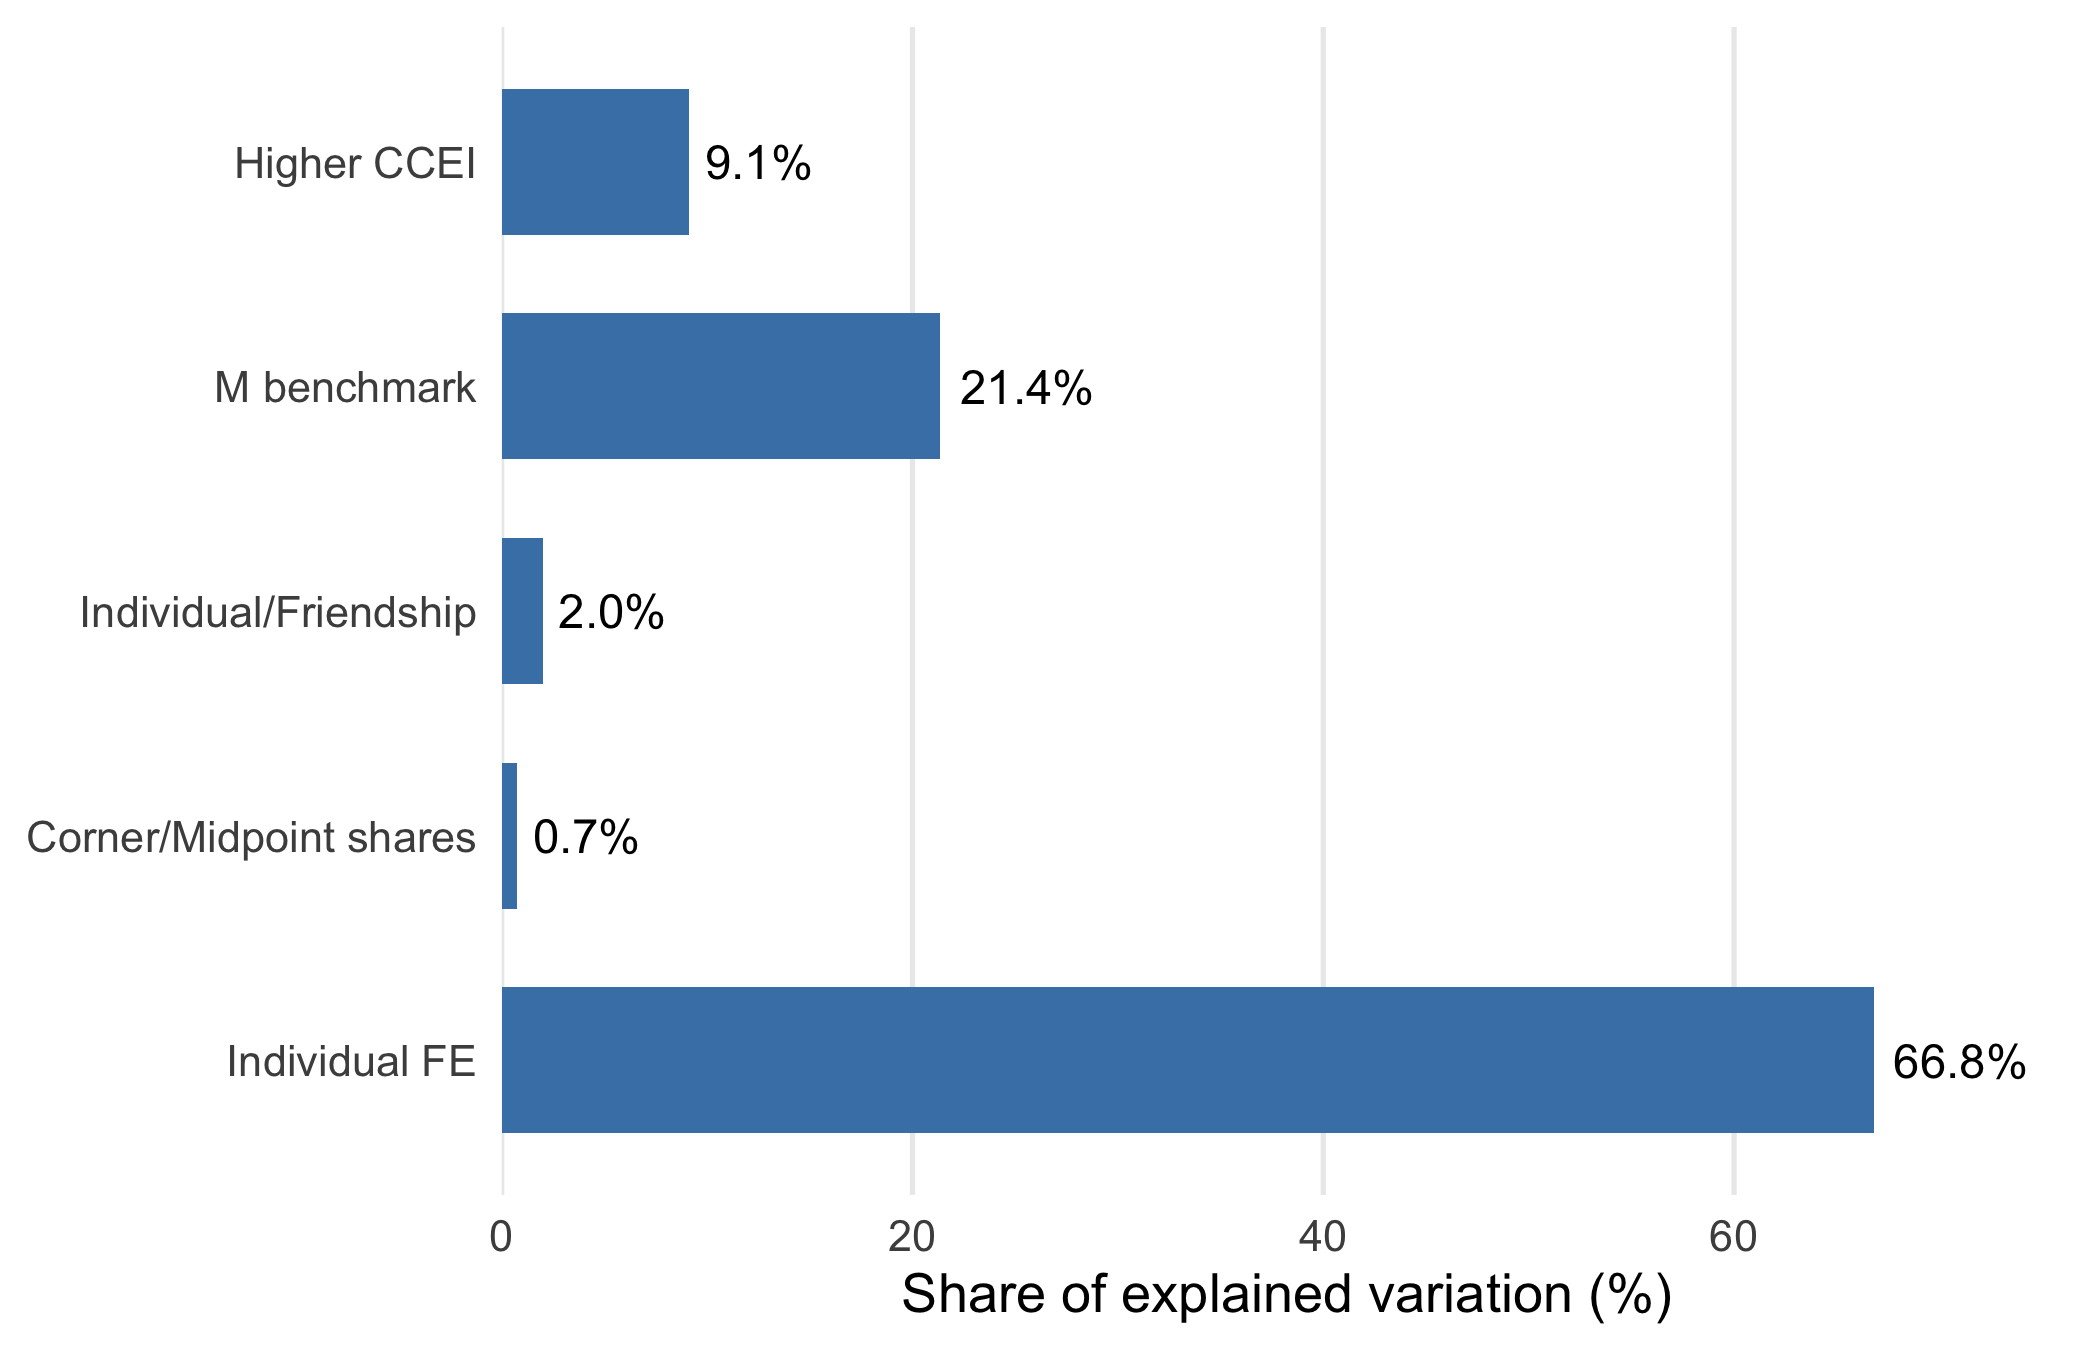
\includegraphics[width=0.85\textwidth]{figures_2025/shapley_bargaining_index_M.png}

\vspace{12pt}
\begin{minipage}{0.9\textwidth}
{\footnotesize \textcolor{red}{\emph{Notes}: Shorrocks--Shapley decomposition of the $R^2$ from Column (3) of \autoref{tab:pref_agg_ccei}, using actual distance $I_{ig}$ and controlling for $M_{ig}$. Blocks are the higher-CCEI indicator, the placebo benchmark, individual and friendship characteristics (including missing-value indicators), corner/midpoint choice shares, and individual fixed effects. Risk-aversion controls are excluded. The respective shares of explained variation are 9.1\%, 21.4\%, 2.0\%, 0.7\%, and 66.8\%.}}
\end{minipage}
\end{figure}


\begin{figure}[H]
\centering
\caption{Parametric Simulation Benchmark for Revealed-Preference Distance}
\label{fig:simulation_V1}
\includegraphics[width=0.72\textwidth]{figures_2025/Ihat_rho0.3and0.7_gi30_gj30_gg30_L200_n50_B100.png}
\vspace{12pt}
\begin{minipage}{\textwidth}
{\footnotesize \emph{Notes}: This figure reports a Monte Carlo benchmark connecting the nonparametric revealed-preference distance to a parametric collective model. For each true preference weight $\alpha \in \{0,0.1,\ldots,1\}$, we generate $B=100$ independent datasets. In each dataset, two individuals face 50 randomly drawn budget sets; on each budget line, choices are made from a 200-point grid of feasible portfolio allocations. Individual utilities are CRRA, with risk-aversion parameters $\rho_1=0.3$ and $\rho_2=0.7$, following the portfolio-choice setting of \citet{Choietal:2007:AER}. Individual choices are drawn from a logit rule over the grid with precision $\gamma=30$, so choices are close to utility maximization and individual CCEIs are high. Group choices are drawn from the same logit rule using the collective utility $U_g=\alpha U_1+(1-\alpha)U_2$, where $\alpha$ is individual 1's true parametric preference weight. For each simulated dataset, we compute the CCEIs for the group dataset, the group dataset combined with individual 1's dataset, the group dataset combined with individual 2's dataset, and the combined dataset containing both individuals and the group; we then calculate $I_{1g}$ using \autoref{eqn:I_ig}. The vertical axis plots $1-I_{1g}$, so larger values indicate closer alignment of collective choices with individual 1's preferences and can be compared directly with $\alpha$. Blue dots denote the Monte Carlo mean of $1-I_{1g}$ across simulations. Shaded bands show the 10--90\% and 5--95\% quantile ranges. The red dashed line is the 45-degree benchmark $y=\alpha$. Red annotations under the x-axis report the share of simulations in which the index is undefined because the denominator in \autoref{eqn:I_ig} is zero.}
\end{minipage}
\end{figure}


\begin{figure}[H]
\centering
\caption{Observed odd--even gaps and random-split benchmark}
\label{fig:taking_turns_cdf}
\begin{subfigure}[b]{0.485\textwidth}
\centering
\includegraphics[width=\textwidth]{figures_2025/taking_turns_cdf_all.png}
\caption{All Pair-Waves}
\end{subfigure}
\hfill
\begin{subfigure}[b]{0.485\textwidth}
\centering
\includegraphics[width=\textwidth]{figures_2025/taking_turns_cdf_bottom25.png}
\caption{Bottom Quartile of Within-Pair Distance Gap}
\end{subfigure}

\vspace{12pt}
\begin{minipage}{\textwidth}
{\footnotesize \emph{Notes}: Panel (a) includes 1,201 selected pair-waves; Panel (b) includes 301 pair-waves in the bottom quartile of the full-index within-pair gap. The blue solid line is the observed CDF; the red dashed line averages 200 placebo CDFs. Shading indicates the pointwise 2.5th--97.5th percentile range across 200 random splits.
}
\end{minipage}
\end{figure}


\begin{figure}[H]
\centering
\caption{First-half versus second-half gaps and random-split benchmark}
\label{fig:taking_turns_first_last}
\begin{subfigure}[b]{0.485\textwidth}
\centering
\includegraphics[width=\textwidth]{figures_2025/taking_turns_first_last_cdf_all.png}
\caption{All Pair-Waves}
\end{subfigure}
\hfill
\begin{subfigure}[b]{0.485\textwidth}
\centering
\includegraphics[width=\textwidth]{figures_2025/taking_turns_first_last_cdf_bottom25.png}
\caption{Bottom Quartile of Within-Pair Distance Gap}
\end{subfigure}

\vspace{12pt}
\begin{minipage}{\textwidth}
{\footnotesize \emph{Notes}: Panel (a) includes 1,201 selected pair-waves; Panel (b) includes 301 pair-waves in the bottom quartile of the full-index within-pair gap. The blue solid line is the observed CDF; the red dashed line averages 200 placebo CDFs. Shading indicates the pointwise 2.5th--97.5th percentile range across 200 random splits.
}
\end{minipage}
\end{figure}

\begin{figure}[H]
\centering
\caption{Distribution of KS p-values: first-half versus second-half gaps}
\label{fig:taking_turns_first_last_ks}
\begin{subfigure}[b]{0.485\textwidth}
\centering
\includegraphics[width=\textwidth]{figures_2025/taking_turns_first_last_ks_pvalues_all.png}
\caption{All Pair-Waves}
\end{subfigure}
\hfill
\begin{subfigure}[b]{0.485\textwidth}
\centering
\includegraphics[width=\textwidth]{figures_2025/taking_turns_first_last_ks_pvalues_bottom25.png}
\caption{Bottom Quartile of Within-Pair Distance Gap}
\end{subfigure}

\vspace{12pt}
\begin{minipage}{\textwidth}
{\footnotesize \emph{Notes}: The panels use the same samples as \autoref{fig:taking_turns_first_last}. Each of 200 random splits produces one asymptotic two-sample KS p-value. Bars show the percentage of splits in each bin. These are descriptive nominal p-values; samples share pair-waves and contain ties. They are not independent tests.
}
\end{minipage}
\end{figure}

\begin{figure}[H]
\centering
\caption{Shorrocks--Shapley Decomposition Of Collective CCEI}
\label{fig:shapley_groupccei}
\includegraphics[width=0.6\textwidth]{figures_2025/shapley_collective_ccei.png}

\vspace{12pt}
\begin{minipage}{\textwidth}
{\footnotesize \emph{Notes}: This figure reports the Shorrocks--Shapley decomposition of the regression $R^2$ from \autoref{tab:collective_ccei}, Column~(4). Explanatory variables are grouped into (i) CCEI variables, (ii) student and friendship characteristics, (iii) individual risk-aversion measures, (iv) individual corner and midpoint choice shares, and (v) pair fixed effects. The CCEI block includes the maximum and absolute within-pair difference of the two members' individual CCEIs. The corner and midpoint share block includes the maximum and absolute within-pair difference of the two members' shares of individual choices made exactly at a corner or at the 50/50 allocation, respectively.}
\end{minipage}
\end{figure}

\begin{figure}[H]
\centering
\caption{Placebo Reassignment Test: CCEI Difference}
\label{fig:placebo_reassignment_cceidiff}

\begin{subfigure}[b]{0.485\textwidth}
\centering
\includegraphics[width=\textwidth]
{figures_2025/placebo_cceidiff_spec1.png}
\caption{Raw index: Class FE}
\end{subfigure}
\hfill
\begin{subfigure}[b]{0.485\textwidth}
\centering
\includegraphics[width=\textwidth]
{figures_2025/placebo_cceidiff_spec2.png}
\caption{\textcolor{red}{Student and friendship controls}}
\end{subfigure}

\begin{subfigure}[b]{0.485\textwidth}
\centering
\includegraphics[width=\textwidth]
{figures_2025/placebo_cceidiff_spec3.png}
\caption{Raw index: Full controls}
\end{subfigure}
\hfill
\begin{subfigure}[b]{0.485\textwidth}
\centering
\includegraphics[width=\textwidth]
{figures_2025/placebo_cceidiff_spec4.png}
\caption{Raw index: Individual FE}
\end{subfigure}

\vspace{12pt}
\begin{minipage}{\textwidth}
{\footnotesize
\emph{Notes}: Each panel shows the distribution of the coefficient on
$CCEI_i-CCEI_j$ across 500 placebo reassignments. Positive values indicate
that member $i$ has a higher individual CCEI than member $j$, while the
difference equals zero when their CCEIs are equal. In each reassignment,
pairs are randomly matched to another pair's group choices within the same
wave and class, and both members of a pair are matched to the same placebo
group. Individual choices and CCEIs are held fixed, while the
revealed-preference distance index is recomputed using the reassigned group
choices. The red dashed line indicates the coefficient estimated using the
actual group choices. \textcolor{red}{Panels (a), (c), and (d) use the baseline, full-controls, and individual-fixed-effects versions,
respectively, of the unadjusted specifications, without $M_{ig}$. Panel (b), highlighted in red,
adds only student and friendship controls to the baseline specification
and is omitted from that table.}
}
\end{minipage}
\end{figure}

\begin{figure}[H]
\centering
\caption{Self-Reported Influence and Alternative Revealed-Preference Distance Measures}
\label{fig:validation_alternative_indices}
\begin{subfigure}[b]{0.485\textwidth}
\centering
\includegraphics[width=\textwidth]{figures_2025/validation_hm_whose_suggestion.png}
\caption{Suggestions: HM-based distance}
\end{subfigure}
\begin{subfigure}[b]{0.485\textwidth}
\centering
\includegraphics[width=\textwidth]{figures_2025/validation_hm_similarity.png}
\caption{Similarity: HM-based distance}
\end{subfigure}
\begin{subfigure}[b]{0.485\textwidth}
\centering
\includegraphics[width=\textwidth]{figures_2025/validation_maxmpi_whose_suggestion.png}
\caption{Suggestions: MaxMPI-based distance}
\end{subfigure}
\begin{subfigure}[b]{0.485\textwidth}
\centering
\includegraphics[width=\textwidth]{figures_2025/validation_maxmpi_similarity.png}
\caption{Similarity: MaxMPI-based distance}
\end{subfigure}
\begin{minipage}{\textwidth}
{\footnotesize \emph{Notes}: Bars report mean revealed-preference distance with 95\% confidence intervals. Panels (a)--(b) use HM-based $I_{ig}$, and Panels (c)--(d) use MaxMPI-based $I_{ig}$. Lower values indicate closer alignment between the individual's choices and the group choices. Panels (b) and (d) restrict the sample to pairs whose absolute difference in individual risk aversion is at or above the pooled sample median.}
\end{minipage}
\end{figure}

\begin{figure}[H]
\centering
\caption{Collective Rationality by Members' Alternative Rationality Measures}
\label{fig:collective_alternative_indices}
\begin{subfigure}[b]{0.485\textwidth}
\centering
\includegraphics[width=\textwidth]{figures_2025/collective_hm_by_member_category_bar.png}
\caption{Mean collective HM index}
\end{subfigure}
\begin{subfigure}[b]{0.485\textwidth}
\centering
\includegraphics[width=\textwidth]{figures_2025/collective_hm_by_member_category_cdf.png}
\caption{CDFs of collective HM index}
\end{subfigure}
\begin{subfigure}[b]{0.485\textwidth}
\centering
\includegraphics[width=\textwidth]{figures_2025/collective_maxmpi_by_member_category_bar.png}
\caption{Mean collective RevMaxMPI}
\end{subfigure}
\begin{subfigure}[b]{0.485\textwidth}
\centering
\includegraphics[width=\textwidth]{figures_2025/collective_maxmpi_by_member_category_cdf.png}
\caption{CDFs of collective RevMaxMPI}
\end{subfigure}
\begin{minipage}{\textwidth}
{\footnotesize \emph{Notes}: Members are classified using the pooled median of the corresponding individual rationality measure. The HM index equals $1-HM/18$, and RevMaxMPI equals $1-MaxMPI$, so higher values indicate greater rationality. Panels (a)--(b) report collective HM outcomes; Panels (c)--(d) report collective RevMaxMPI outcomes. Bars report means with 95\% confidence intervals. Difference labels report pairwise two-sample $t$-tests. +, *, and ** denote $p<0.10$, $p<0.05$, and $p<0.01$, respectively.}
\end{minipage}
\end{figure}

\begin{figure}[H]
\centering
\caption{CDFs of Individual and Group HM Indices}
\label{fig:cdf_hm_individual_group}
\begin{subfigure}[b]{0.485\textwidth}
\centering
\includegraphics[width=\textwidth]{figures_2025/figure_individual_hm_index_cdf_baseline_endline.png}
\caption{Individual HM index}
\end{subfigure}
\begin{subfigure}[b]{0.485\textwidth}
\centering
\includegraphics[width=\textwidth]{figures_2025/figure_group_hm_index_cdf_baseline_endline.png}
\caption{Group HM index}
\end{subfigure}
\begin{minipage}{\textwidth}
{\footnotesize \emph{Notes}: The HM index is defined as one minus the minimum number of observations that must be removed to satisfy GARP, divided by 18. Higher values therefore indicate greater rationality. The panels report empirical CDFs separately for the baseline and endline.}
\end{minipage}
\end{figure}


\begin{figure}[H]
\centering
\caption{CDFs of Individual and Group RevMaxMPI}
\label{fig:cdf_revmaxmpi_individual_group}
\begin{subfigure}[b]{0.485\textwidth}
\centering
\includegraphics[width=\textwidth]{figures_2025/figure_individual_revmaxmpi_cdf_baseline_endline.png}
\caption{Individual RevMaxMPI}
\end{subfigure}
\begin{subfigure}[b]{0.485\textwidth}
\centering
\includegraphics[width=\textwidth]{figures_2025/figure_group_revmaxmpi_cdf_baseline_endline.png}
\caption{Group RevMaxMPI}
\end{subfigure}
\begin{minipage}{\textwidth}
{\footnotesize \emph{Notes}: RevMaxMPI is defined as one minus MaxMPI, so higher values indicate greater rationality. The panels report empirical CDFs separately for the baseline and endline.}
\end{minipage}
\end{figure}

\begin{figure}[H]
\centering
\caption{Histograms of Alternative Revealed-Preference Distance Measures}
\label{fig:hist_alternative_rp_distance}
\begin{subfigure}[b]{0.485\textwidth}
\centering
\includegraphics[width=\textwidth]{figures_2025/hist_revealed_preference_distance_hm_bothhigh.png}
\caption{HM index: ties assigned High}
\end{subfigure}
\begin{subfigure}[b]{0.485\textwidth}
\centering
\includegraphics[width=\textwidth]{figures_2025/hist_revealed_preference_distance_hm_bothlow.png}
\caption{HM index: ties assigned Low}
\end{subfigure}
\begin{subfigure}[b]{0.485\textwidth}
\centering
\includegraphics[width=\textwidth]{figures_2025/hist_revealed_preference_distance_maxmpi_bothhigh.png}
\caption{RevMaxMPI: ties assigned High}
\end{subfigure}
\begin{subfigure}[b]{0.485\textwidth}
\centering
\includegraphics[width=\textwidth]{figures_2025/hist_revealed_preference_distance_maxmpi_bothlow.png}
\caption{RevMaxMPI: ties assigned Low}
\end{subfigure}
\begin{minipage}{\textwidth}
{\footnotesize \emph{Notes}: The panels report the distributions of revealed-preference distance for more- and less-rational members. Panels (a)--(b) use the HM index and HM-based $I_{ig}$; Panels (c)--(d) use RevMaxMPI and MaxMPI-based $I_{ig}$. Panels (a) and (c) assign both members to the more-rational category when their indices are tied, whereas Panels (b) and (d) assign both to the less-rational category. Each distribution is normalized to percentage shares within the corresponding member category. Lower values of $I_{ig}$ indicate closer alignment between the individual's choices and the group choices.}
\end{minipage}
\end{figure}


\begin{figure}[H]
\centering
\caption{Distribution of KS p-values: odd--even gaps}
\label{fig:taking_turns_ks}
\begin{subfigure}[b]{0.485\textwidth}
\centering
\includegraphics[width=\textwidth]{figures_2025/taking_turns_ks_pvalues_all.png}
\caption{All Pair-Waves}
\end{subfigure}
\hfill
\begin{subfigure}[b]{0.485\textwidth}
\centering
\includegraphics[width=\textwidth]{figures_2025/taking_turns_ks_pvalues_bottom25.png}
\caption{Bottom Quartile of Within-Pair Distance Gap}
\end{subfigure}

\vspace{12pt}
\begin{minipage}{\textwidth}
{\footnotesize \emph{Notes}: The panels use the same samples as \autoref{fig:taking_turns_cdf}. Each of 200 random splits produces one asymptotic two-sample KS p-value. Bars show the percentage of splits in each bin. These are descriptive nominal p-values; samples share pair-waves and contain ties. They are not independent tests.
}
\end{minipage}
\end{figure}

\begin{figure}[H]
\centering
\caption{Shorrocks--Shapley Decomposition Of Alternative Collective Rationality Indices}
\label{fig:shapley_collective_alternative_indices}
\begin{subfigure}[b]{0.485\textwidth}
\centering
\includegraphics[width=\textwidth]{figures_2025/shapley_collective_hm.png}
\caption{Collective HM index}
\end{subfigure}
\begin{subfigure}[b]{0.485\textwidth}
\centering
\includegraphics[width=\textwidth]{figures_2025/shapley_collective_revmaxmpi.png}
\caption{Collective RevMaxMPI}
\end{subfigure}

\vspace{12pt}
\begin{minipage}{\textwidth}
{\footnotesize \emph{Notes}: This figure reports robustness checks for the Shorrocks--Shapley decomposition of the regression $R^2$ from the specifications corresponding to \autoref{tab:collective_ccei}, Column~(4). Panel (a) uses the collective HM index as the dependent variable and groups the maximum and absolute within-pair difference of the members' HM indices into the rationality-index block. Panel (b) uses collective RevMaxMPI as the dependent variable and groups the maximum and absolute within-pair difference of the members' RevMaxMPI measures into that block. Both indices are defined so that higher values indicate greater rationality. The remaining blocks contain (ii) student and friendship characteristics, (iii) individual risk-aversion measures, (iv) individual corner and midpoint choice shares, and (v) pair fixed effects. The corner and midpoint share block includes the maximum and absolute within-pair difference of the two members' shares of individual choices made exactly at a corner or at the 50/50 allocation, respectively.}
\end{minipage}
\end{figure}


\begin{figure}[H]
\centering
\caption{Shorrocks--Shapley Decomposition of $C_{Ng}$}
\label{fig:shapley_collective_cng}
\includegraphics[width=0.6\textwidth]{figures_2025/shapley_collective_cNg.png}

\vspace{12pt}
\begin{minipage}{\textwidth}
{\footnotesize \emph{Notes}: This figure reports the Shorrocks--Shapley decomposition of the regression $R^2$ from the pair fixed-effects specification in which the CCEI-based cross-consistency cost $C_{Ng}$ is the dependent variable. Explanatory variables are grouped into (i) individual CCEI variables, (ii) student and friendship characteristics, (iii) individual risk-aversion measures, (iv) individual corner and midpoint choice shares, and (v) pair fixed effects. The individual CCEI block includes the maximum and absolute within-pair difference of the two members' individual CCEIs. The decomposition is descriptive.}
\end{minipage}
\end{figure}

\begin{figure}[H]
\centering
\caption{Shorrocks--Shapley Decomposition of Alternative Cross-Consistency Costs}
\label{fig:shapley_collective_cng_alternative_indices}
\begin{subfigure}[b]{0.485\textwidth}
\centering
\includegraphics[width=\textwidth]{figures_2025/shapley_collective_cNg_hm.png}
\caption{HM cross-consistency cost}
\end{subfigure}
\begin{subfigure}[b]{0.485\textwidth}
\centering
\includegraphics[width=\textwidth]{figures_2025/shapley_collective_cNg_revmaxmpi.png}
\caption{MaxMPI cross-consistency cost}
\end{subfigure}

\vspace{12pt}
\begin{minipage}{\textwidth}
{\footnotesize \emph{Notes}: This figure reports robustness checks for the Shorrocks--Shapley decomposition in \autoref{fig:shapley_collective_cng}. Panel (a) uses the HM cross-consistency cost $C^{HM}_{Ng}$ as the dependent variable and groups the maximum and absolute within-pair difference of the members' HM indices into the rationality-index block. Panel (b) uses the MaxMPI cross-consistency cost $C^{MP}_{Ng}$ as the dependent variable and groups the maximum and absolute within-pair difference of the members' RevMaxMPI measures into that block. The HM index and RevMaxMPI are defined so that higher values indicate greater individual rationality, whereas lower cross-consistency costs indicate greater consistency between individual and group choices. The remaining blocks contain student and friendship characteristics, individual risk-aversion measures, individual corner and midpoint choice shares, and pair fixed effects.}
\end{minipage}
\end{figure}



\begin{comment}
\begin{landscape}
\begin{figure}[H]
\small
\centering
\caption{Selected Individuals For Illustration}
\label{fig:selected_individuals}
\subfigure[Panel (a)]{%
  \centering
  \includegraphics[width=0.7\textwidth]{figures_2025/relconsumption1110116_Baseline.png}
}
\subfigure[Panel (b)]{%
  \centering
  \includegraphics[width=0.7\textwidth]{figures_2025/relconsumption1110123_Baseline.png}
}
\subfigure[Panel (c)]{%
  \centering
  \includegraphics[width=0.7\textwidth]{figures_2025/relconsumption1110128_Baseline.png}
}
\subfigure[Panel (d)]{%
  \centering
  \includegraphics[width=0.7\textwidth]{figures_2025/relconsumption1110224_Baseline.png}
}
\begin{minipage}{\textwidth}
{\footnotesize \emph{Notes}: This figure illustrates portfolio choices for four groups, selected to highlight heterogeneity in behavior. Each combined figure displays the decisions of two members within the same group: the left panel represents the stayer, while the right panel represents the mover. Individual decisions are shown as colored circles, while collective (group) decisions are shown as black crosses (X). The blue markers indicate the more rational individual, whereas the red markers indicate the less rational individual.}
\end{minipage}
\end{figure}
\end{landscape}

\begin{figure}[H]
\centering
\includegraphics[width=0.8\textwidth]{figures_2025/ccei_bargaining_had_individual_low.png}
\caption{Low RA Difference Sample}\label{figure:ccei_bargainig_individual_low}
\end{figure}

\end{comment}



\newpage
\section{Additional Tables}\label{appendix:tables}

\begin{table}[H]
\centering
\small
\singlespacing
\renewcommand{\arraystretch}{1.05}
\caption{Sensitivity to Buffers around Corner and Equal-Allocation Choices}
\label{tab:pref_agg_ccei_buffers}
\begin{tabular*}{\textwidth}{@{\extracolsep{\fill}}lcccc}
\toprule
& \multicolumn{2}{c}{Higher-CCEI indicator} & \multicolumn{2}{c}{CCEI difference} \\
\cmidrule(lr){2-3}\cmidrule(lr){4-5}
Dependent variable: $I_{ig}$ & (1) & (2) & (3) & (4) \\
\midrule
\csname @@input\endcsname tables_2025/table_bargainingCCEI_buffers_M.tex
\midrule
Observations & 2,512 & 2,512 & 2,512 & 2,512 \\
Fixed effects & Class & Individual & Class & Individual \\
Individual and friendship controls & \checkmark & \checkmark & \checkmark & \checkmark \\
Corner/equal-allocation share controls & \checkmark & \checkmark & \checkmark & \checkmark \\
\bottomrule
\end{tabular*}
\begin{minipage}{\textwidth}
{\footnotesize \emph{Notes}:   The table reports results from estimating \autoref{eqn:individual_distance}. In Columns (1)--(2), the higher-CCEI indicator equals one for both members when their individual CCEIs are equal. Columns (3)--(4) replace this indicator with $CCEI_i-CCEI_j$. Panel A reproduces the coefficients and standard errors in Columns (2), (3), (5), and (6) of \autoref{tab:pref_agg_ccei}, respectively. Panels B and C change only the definitions of the corner and equal-allocation choice shares. Let $q=x/(x+y)$ be the share of total payoff allocated to the first account. For buffer $b$, a choice is classified as a corner if $q\leq b$ or $q\geq 1-b$, and as an equal allocation if $|q-0.5|\leq b$. Panels A, B, and C use $b=0$, $0.025$, and $0.05$, respectively. Each specification controls for the member's share of each choice pattern and its signed member-minus-partner difference, together with individual and friendship characteristics; risk aversion and its within-pair difference are excluded. The revealed-preference distance $I_{ig}$ is undefined when the total cost, $c_{Ng}$, is zero; the common balanced sample retains only pairs for which $I_{ig}$ is defined in both waves, yielding 2,512 student-wave observations from 1,256 students in 628 pairs. Columns (1) and (3) include class fixed effects and gender-composition controls, with same-sex pairs as the omitted category. Columns (2) and (4) include individual fixed effects, which absorb gender composition. Standard errors are clustered at the class level and presented in parentheses. +, *, ** denote significance at the 10\%, 5\%, and 1\% levels, respectively.}
\end{minipage}
\end{table}

\begin{landscape}
\begin{table}[H]
\centering
\footnotesize
\begin{threeparttable}
\caption{Correlation Table}
\label{tab:corr_ihat}
\input{tables_2025/table_correlation_IminusM}
\begin{tablenotes}[flushleft]
\footnotesize
\item[] \emph{Notes}: This table reports pairwise correlations among baseline
individual characteristics. The distance column uses the placebo-adjusted index $I^*_{ig}=I_{ig}-M_{ig}$. +, *, and ** denote significance at the 10\%, 5\%, and
1\% levels, respectively.
\end{tablenotes}
\end{threeparttable}
\end{table}
\end{landscape}

\begin{table}[H]
\centering
\singlespacing
\caption{Individual Rationality and Revealed-Preference Distance by Mover Status}
\label{tab:bargaining_ccei_ihat_mover}
\footnotesize
\setlength{\tabcolsep}{3pt}
\renewcommand{\arraystretch}{1.1}
\resizebox{\textwidth}{!}{%
\begin{tabular}{lcccccc}
\toprule
& \multicolumn{3}{c}{Ties Assigned High} & \multicolumn{3}{c}{CCEI Difference} \\
\cmidrule(lr){2-4}\cmidrule(lr){5-7}
Dependent variable: $I_{ig}$ & (1) & (2) & (3) & (4) & (5) & (6) \\
\midrule
\input{tables_2025/table_bargainingCCEI_mover_M}
\end{tabular}}
\begin{minipage}{\textwidth}
\footnotesize
\emph{Notes}:   Each column augments the corresponding specification in \autoref{tab:pref_agg_ccei} with mover status and its interaction with the rationality measure. The higher-CCEI indicator equals one for both members in a tie. All columns use the same balanced sample of 2,512 student-wave observations. Columns (1), (2), (4), and (5) include class fixed effects; Columns (3) and (6) include individual fixed effects, which absorb the time-invariant mover and gender-composition indicators. Columns (2), (3), (5), and (6) include individual and friendship characteristics and exact corner and equal-allocation shares, together with their within-pair differences. Risk aversion and its within-pair difference are excluded. The interaction tests whether the rationality--distance relationship differs by mover status. The continuous-gap interaction is numerically near zero in Column (4) by pair symmetry; rounded zeros should not be interpreted as separately informative effects. Standard errors are clustered at the class level and reported in parentheses. +, *, and ** denote significance at the 10\%, 5\%, and 1\% levels, respectively.
\end{minipage}
\end{table}

\begin{table}[H]
\centering
\singlespacing
\caption{Individual Characteristics and Changes in CCEI}
\label{tab:individual_ccei_change}
\small
\renewcommand{\arraystretch}{1.05}
\begin{tabular*}{0.9\textwidth}{@{\extracolsep{\fill}}lcc}
\toprule
Dependent variable: $\Delta CCEI_i$ & (1) & (2) \\
 & Baseline characteristics & Baseline and changes \\
\midrule
\input{tables_2025/table_individual_ccei_change}
\end{tabular*}
\par\smallskip
\begin{minipage}{\textwidth}
\footnotesize
\emph{Notes}: The dependent variable is the change in individual CCEI from baseline to endline. Each column reports an individual-level OLS regression using the 1,256 students in the balanced sample of \autoref{tab:pref_agg_ccei}, with one observation per student. Column (1) includes baseline gender, height, math score, the five personality measures, and friendship-network out-degree and in-degree. Column (2) additionally includes endline-minus-baseline changes in math score, out-degree, and in-degree. Neither specification includes class fixed effects, partner characteristics, within-pair differences, risk aversion, or choice-pattern shares. Missing baseline math and personality values are set to zero, with corresponding missing-value indicators included; their coefficients and the constant are omitted from the display. Standard errors are clustered across 64 classes and reported in parentheses. +, *, and ** denote significance at the 10\%, 5\%, and 1\% levels, respectively.
\end{minipage}
\end{table}

\begin{table}[H]
\centering
\singlespacing
\caption{Alternative Measures of Rationality and Preference Distance \mbox{(Updated)}}
\label{tab:pref_agg_alternatives}
\label{tab:pref_agg_hm}
\label{tab:pref_agg_maxmpi}
\label{tab:pref_agg_ra_index}
\footnotesize
\setlength{\tabcolsep}{3pt}
\renewcommand{\arraystretch}{1.0}
\resizebox{\textwidth}{!}{%
\begin{tabular}{lcccccc}
\toprule
& \multicolumn{3}{c}{Ties Assigned High} & \multicolumn{3}{c}{Rationality Difference} \\
\cmidrule(lr){2-4}\cmidrule(lr){5-7}
& (1) & (2) & (3) & (4) & (5) & (6) \\
\midrule
\csname @@input\endcsname tables_2025/table_bargaining_alternatives_M.tex
\end{tabular}}
\begin{minipage}{\textwidth}
\footnotesize
\emph{Notes}: \textcolor{red}{Every column retains actual distance as the outcome and controls for its measure-specific placebo benchmark $M_{ig}$.}  Panels A and B use HM- and MaxMPI-based revealed-preference distance; Panel C uses normalized risk-aversion distance from \eqref{eqn:simple_measure}. Columns (1)--(3) assign both members the higher-rationality indicator in a tie; Columns (4)--(6) use the rationality difference. In Panel A, $FGARP_i=1-HM_i/18$, where $HM_i$ counts observations removed to restore GARP; the continuous regressor is $HM_j-HM_i=18(FGARP_i-FGARP_j)$. Panel B uses $RevMaxMPI_i=1-MaxMPI_i$, and Panel C uses CCEI. Panels A and B retain students with distance defined in both waves (2,512 observations); Panel C includes all 2,604 observations with defined distance, retaining four singleton students under individual fixed effects. Specifications and controls follow \autoref{tab:pref_agg_ccei}: risk aversion and its within-pair difference are excluded, and corner/equal-allocation shares use exact choices. Individual fixed effects absorb gender composition. \textcolor{red}{Panels A and B are provisional: HM uses 50 sampled donors and MaxMPI uses 20. MaxMPI donor calculations exceeding two seconds receive distance one half (2.0\% on average). Panel C uses all 651 non-own donors.} Other control coefficients are omitted. Standard errors are clustered at the class level and reported in parentheses. +, *, and ** denote significance at the 10\%, 5\%, and 1\% levels, respectively.
\end{minipage}
\end{table}


\begin{table}[H]
\centering
\caption{Summary Statistics of Alternative Rationality Measures}
\label{tab:alternative_indices_summary}
\begin{tabular}{lrrrrrr}
\toprule
& (1) & (2) & (3) & (4) & (5) & (6) \\
\input{tables_2025/table_alternative_indices_summary}
\end{tabular}
\begin{minipage}{\textwidth}
{\footnotesize \emph{Notes}: The HM index is one minus the minimum number of observations that must be removed to satisfy GARP, divided by 18. RevMaxMPI is one minus MaxMPI. Thus, higher values of both measures indicate greater rationality. HM-based and MaxMPI-based $I_{ig}$ are constructed from the corresponding cross-index costs. Lower values of $I_{ig}$ indicate closer alignment between the individual's choices and the group choices.}
\end{minipage}
\end{table}


\begin{table}[H]
\centering
\caption{Disjoint-Choice Test}
\label{tab:disjoint_choice}
% The retained table remains visible until the full 500-partition build is ready.
\IfFileExists{tables_2025/table_disjoint_choice.tex}{%
\input{tables_2025/table_disjoint_choice.tex}
}{%
\begin{tabular}{lcc}
\toprule
Estimate & Median & 95\% range \\
\midrule
\multicolumn{3}{l}{\emph{Panel A: Higher-CCEI indicator}} \\
\textcolor{red}{Raw index: baseline}
    & $-0.168$ & $[-0.216,\,-0.120]$ \\
\textcolor{red}{Student and friendship controls}
    & $-0.164$ & $[-0.212,\,-0.117]$ \\
\textcolor{red}{Raw index: full controls}
    & $-0.139$ & $[-0.192,\,-0.087]$ \\
\textcolor{red}{Raw index: individual FE}
    & $-0.082$ & $[-0.205,\,\phantom{-}0.026]$ \\
\midrule
\multicolumn{3}{l}{\emph{Panel B: Continuous CCEI difference}} \\
Both directions
    & $-0.832$ & $[-1.066,\,-0.586]$ \\
\bottomrule
\end{tabular}

\begin{minipage}{\textwidth}
{\footnotesize \emph{Notes}: For each pair-wave observation, the 18 choices of each member and the 18 group choices are independently divided into two sets of nine. In the $A\rightarrow B$ analysis, individual choices in set $A$ are used to determine the higher-CCEI member and to construct the individual risk-aversion and corner/midpoint-share controls, while choices in set $B$ are used to construct the dependent variable. The $B\rightarrow A$ analysis reverses the roles of the two sets. \textcolor{red}{Rows 1--4 of Panel A are raw-distance diagnostic regressions with class fixed effects alone, student and friendship controls, full controls, and individual fixed effects, respectively. They omit the placebo benchmark $M_{ig}$.} Observations for which the two members have equal CCEIs in the set used to determine relative rationality are omitted because the higher-CCEI member is undefined. The median coefficients are negative in all four specifications. \textcolor{red}{The 95\% ranges for the first three rows lie below zero, whereas the range for the individual-fixed-effects specification in the fourth row includes zero.} In Panel B, the absolute within-pair CCEI difference calculated from one set is used to explain the difference in the two members' revealed-preference distance indices calculated from the other set. The difference in revealed-preference distance is defined as the higher-CCEI member's distance minus the lower-CCEI member's distance. The Panel B regressions include no additional controls or fixed effects, and standard errors are clustered at the class level. Both panels pool the coefficient estimates from the $A\rightarrow B$ and $B\rightarrow A$ analyses; each reported row therefore summarizes 1,000 coefficient estimates, with 500 from each direction. All Panel B estimates are negative. The 95\% range reports the 2.5th and 97.5th percentiles of the corresponding coefficient distribution.}
\end{minipage}
}
\end{table}


\begin{table}[H]
\centering
\caption{Individual Rationality and Revealed-Preference Distance: Ties Assigned Low \mbox{(Updated)}}
\label{tab:pref_agg_ccei_bothlow}
\begin{tabular}{lccc}
\toprule \hline
Dependent variable: $I_{ig}$ & (1) & (2) & (3) \\ \midrule
\input{tables_2025/table_bargainingCCEI_bothlow_M}
\end{tabular}
\begin{minipage}{\textwidth}
{\footnotesize \emph{Notes}: \textcolor{red}{Every column retains actual distance as the outcome and controls for its measure-specific placebo benchmark $M_{ig}$.}  The table repeats the main analysis while assigning both members to the lower-CCEI category when their individual CCEIs are equal. Columns (1)--(2) include class fixed effects, and Column (3) includes individual fixed effects. Columns (2)--(3) include the full set of individual, friendship, and corner/midpoint-share controls; risk-aversion controls are excluded. Gender-composition controls are included in Column (2), with same-sex pairs as the omitted category, and are absorbed by individual fixed effects in Column (3). The balanced sample contains 2,512 student-wave observations from 1,256 students in 628 pairs. Standard errors are clustered at the class level and presented in parentheses. +, *, ** denote significance at the 10\%, 5\%, and 1\% levels, respectively.}
\end{minipage}
\end{table}

\begin{table}[H]
\centering
\singlespacing
\small
\caption{Individual Rationality and Collective Outcomes}
\label{tab:collective_ccei_ceiv_categories}
\setlength{\tabcolsep}{9pt}
\renewcommand{\arraystretch}{1.12}
\input{tables_2025/collective_ccei_ceiv_categories.tex}
\par\vspace{8pt}
\begin{minipage}{\textwidth}
\footnotesize
\emph{Notes}: OLS regression coefficients have class-clustered standard errors in parentheses. All columns
use 1,304 pair-waves from 652 pairs in 64 classes. Low--Low is omitted. High means individual CCEI exceeds
the pooled median across both waves (0.9806594), and Low otherwise, as in \autoref{fig:collective_ccei_ceiv_categories}. Column (1) includes
class fixed effects; Column (2) adds full controls with class fixed effects; Column (3) uses full controls
with pair fixed effects.

The post-estimation section reports the linear contrast $\beta_{HH}-\beta_{LH}$ and its class-clustered
standard error; the contrast is not an additional regressor. Its two-sided $p$-value tests
$H_0:\beta_{HH}=\beta_{LH}$ using the estimated coefficient covariance.

Full controls comprise pair maxima and absolute differences in math score, height, Big Five traits,
network degree, popularity, and exact corner/equal-allocation shares, with mixed-gender, friendship,
and missing-value indicators. Risk-aversion controls and wave fixed effects are excluded.
Estimates and category comparisons describe conditional associations. +, *, and ** denote significance
at the 10\%, 5\%, and 1\% levels.
\end{minipage}
\end{table}

%%%%%%%%%

\begin{table}[H]
\centering
\footnotesize
\begin{threeparttable}
\caption{Classification Analysis Of HighCCEI (Random Forest)}\label{tab:clan_clb_rf}
\begin{tabular}{lccc}
\toprule \hline
 & 20\% Most ($\delta_5$) & 20\% Least ($\delta_1$) & Difference ($\delta_5-\delta_1$) \\
\midrule
height\_diff & -0.702 & 0.134 & -0.820 \,[0.180] \\
& ( -2.261,\,0.851 ) & ( -1.316,\,1.547 ) & ( -3.098,\,1.443 ) \\
\addlinespace
height\_i & 161.783 & 164.851 & -2.994 \,[0.002] \\
& ( 160.246,\,163.330 ) & ( 163.237,\,166.434 ) & ( -4.894,\,-1.189 ) \\
\addlinespace
inclass\_n\_diff & -0.189 & 0.068 & -0.233 \,[0.105] \\
& ( -0.724,\,0.339 ) & ( -0.376,\,0.480 ) & ( -0.969,\,0.486 ) \\
\addlinespace
inclass\_n\_friends & 4.522 & 5.248 & -0.764 \,[0.012] \\
& ( 4.005,\,5.026 ) & ( 4.808,\,5.676 ) & ( -1.377,\,-0.149 ) \\
\addlinespace
inclass\_pop\_diff & -0.394 & 0.314 & -0.696 \,[0.066] \\
& ( -1.023,\,0.283 ) & ( -0.141,\,0.808 ) & ( -1.502,\,0.110 ) \\
\addlinespace
inclass\_popularity & 4.183 & 5.543 & -1.370 \,[0.000] \\
& ( 3.652,\,4.707 ) & ( 5.054,\,6.015 ) & ( -2.079,\,-0.678 ) \\
\addlinespace
math\_diff & -0.134 & 0.161 & -0.258 \,[0.081] \\
& ( -0.477,\,0.206 ) & ( -0.114,\,0.424 ) & ( -0.715,\,0.184 ) \\
\addlinespace
mathscore\_dist\_missing & 0.000 & 0.050 & -0.043 \,[0.274] \\
& ( 0.000,\,0.000 ) & ( -0.033,\,0.126 ) & ( -0.121,\,0.035 ) \\
\addlinespace
mathscore\_i & 2.425 & 3.050 & -0.621 \,[0.001] \\
& ( 2.163,\,2.694 ) & ( 2.750,\,3.334 ) & ( -1.005,\,-0.255 ) \\
\addlinespace
post & 0.398 & 0.671 & -0.273 \,[0.000] \\
& ( 0.327,\,0.469 ) & ( 0.597,\,0.752 ) & ( -0.380,\,-0.166 ) \\
\addlinespace 
\hline \bottomrule
\end{tabular}
\end{threeparttable}
\begin{minipage}{\textwidth}
{\footnotesize \emph{Notes}: Entries are medians over 250 splits. Confidence intervals are in parentheses. $p$-values for the null that the difference equals zero are reported in brackets. This appendix reports the full Classification Analysis (CLAN) results summarized in \autoref{section:results}. Following \citet{chernozhukov2018generic}, we train a random forest to predict the revealed-preference-distance outcome from a wide set of pair- and individual-level characteristics, rank observations by their predicted heterogeneity, and compare characteristic means in the top 20\% ($\delta_5$) and bottom 20\% ($\delta_1$) of the ranking. Estimates are medians over 250 sample splits, with bootstrap confidence intervals in parentheses and $p$-values for the null that the difference equals zero in brackets.

The pair-level differences in status dimensions (\texttt{height\_diff}, \texttt{inclass\_pop\_diff}, \texttt{math\_diff}) are themselves only marginally significant, reinforcing that what matters is the absolute endowment of the more rational member, not the gap between members. Among the Big Five traits, only the more rational member's own \emph{agreeableness} ($+0.31$, $p = 0.026$) and \emph{emotional stability} ($+0.28$, $p = 0.041$) load on the high-heterogeneity bin, while pair-level differences in personality traits and the remaining three dimensions (openness, extraversion, conscientiousness) are statistically indistinguishable across the two groups. Together with the pre-specified subgroup analysis in \autoref{section:results}, the CLAN exercise points to a coherent picture: the rationality--distance relationship is strongest at baseline, in pairs where the more rational member lacks other status advantages, and is amplified by prosocial temperament; the PBL intervention attenuates this relationship, consistent with rationality becoming more evenly distributed across pair members after the program.}
\end{minipage}
\end{table}


\begin{table}[H]
\centering
\footnotesize
\begin{threeparttable}
\caption{Classification Analysis Of HighCCEI (Random Forest), Continued}\label{tab:clan_clb_rf2}
\begin{tabular}{lccc}
\toprule \hline
 & 20\% Most ($\delta_5$) & 20\% Least ($\delta_1$) & Difference ($\delta_5-\delta_1$) \\
\midrule
agreeable\_diff & 0.009 & 0.020 & -0.006 \,[0.163] \\
& ( -0.149,\,0.165 ) & ( -0.114,\,0.154 ) & ( -0.222,\,0.209 ) \\
\addlinespace
agreeable\_diff\_missing & 0.000 & 0.050 & -0.043 \,[0.274] \\
& ( 0.000,\,0.000 ) & ( -0.033,\,0.126 ) & ( -0.121,\,0.035 ) \\
\addlinespace
agreeable\_i & 2.944 & 2.624 & 0.309 \,[0.026] \\
& ( 2.807,\,3.076 ) & ( 2.378,\,2.871 ) & ( 0.038,\,0.588 ) \\
\addlinespace
conscientious\_diff & -0.022 & 0.019 & -0.034 \,[0.156] \\
& ( -0.185,\,0.149 ) & ( -0.167,\,0.183 ) & ( -0.294,\,0.218 ) \\
\addlinespace
conscientious\_diff\_missing & 0.000 & 0.050 & -0.043 \,[0.274] \\
& ( 0.000,\,0.000 ) & ( -0.033,\,0.126 ) & ( -0.121,\,0.035 ) \\
\addlinespace
conscientious\_i & 3.387 & 3.239 & 0.161 \,[0.270] \\
& ( 3.239,\,3.547 ) & ( 2.935,\,3.537 ) & ( -0.173,\,0.472 ) \\
\addlinespace
opened\_diff & -0.034 & 0.003 & -0.031 \,[0.171] \\
& ( -0.226,\,0.158 ) & ( -0.151,\,0.160 ) & ( -0.298,\,0.229 ) \\
\addlinespace
opened\_diff\_missing & 0.000 & 0.050 & -0.043 \,[0.274] \\
& ( 0.000,\,0.000 ) & ( -0.033,\,0.126 ) & ( -0.121,\,0.035 ) \\
\addlinespace
opened\_i & 3.509 & 3.418 & 0.087 \,[0.368] \\
& ( 3.349,\,3.666 ) & ( 3.113,\,3.735 ) & ( -0.268,\,0.429 ) \\
\addlinespace
outgoing\_diff & -0.034 & 0.014 & -0.059 \,[0.189] \\
& ( -0.281,\,0.209 ) & ( -0.152,\,0.184 ) & ( -0.360,\,0.261 ) \\
\addlinespace
outgoing\_diff\_missing & 0.000 & 0.050 & -0.043 \,[0.274] \\
& ( 0.000,\,0.000 ) & ( -0.033,\,0.126 ) & ( -0.121,\,0.035 ) \\
\addlinespace
outgoing\_i & 3.478 & 3.467 & -0.009 \,[0.396] \\
& ( 3.303,\,3.651 ) & ( 3.141,\,3.803 ) & ( -0.384,\,0.378 ) \\
\addlinespace
stable\_diff & 0.019 & -0.034 & 0.053 \,[0.286] \\
& ( -0.160,\,0.191 ) & ( -0.183,\,0.113 ) & ( -0.198,\,0.312 ) \\
\addlinespace
stable\_diff\_missing & 0.000 & 0.050 & -0.043 \,[0.274] \\
& ( 0.000,\,0.000 ) & ( -0.033,\,0.126 ) & ( -0.121,\,0.035 ) \\
\addlinespace
stable\_i & 2.581 & 2.301 & 0.280 \,[0.041] \\
& ( 2.447,\,2.714 ) & ( 2.061,\,2.528 ) & ( 0.011,\,0.553 ) \\
\addlinespace
\hline \bottomrule
\end{tabular}
\end{threeparttable}
\begin{minipage}{\textwidth}
{\footnotesize \emph{Notes}: Entries are medians over 250 splits. Confidence intervals are in parentheses. $p$-values for the null that the difference equals zero are reported in brackets.}
\end{minipage}
\end{table}

\begin{table}[H]
\centering
\caption{Main estimates after excluding turn-like pair-waves}
\label{tab:taking_turns_exclusion}
\begin{tabular}{lcccc}
\toprule \hline
Dependent variable: $I_{ig}$ & (1) & (2) & (3) & (4) \\ \midrule
\multicolumn{5}{l}{Panel A: Full sample} \\
\input{tables_2025/table_taking_turns_exclusion}
\end{tabular}
\begin{minipage}{\textwidth}
{\footnotesize \emph{Notes}: \textcolor{red}{These are retained raw-index results without $M_{ig}$; an updated counterpart is not yet available in the review outputs.}  The dependent variable is revealed-preference distance. Columns (1)--(4) follow the corresponding specifications in \autoref{tab:pref_agg_ccei}, with the same controls and fixed effects. Panel A reports the full-sample estimates; Panel B excludes both members of 51 turn-like pair-waves. Classification uses the pair-specific 95th percentile across 200 random splits. Standard errors are clustered at the class level and presented in parentheses. +, *, ** denote significance at the 10\%, 5\%, and 1\% levels, respectively.
}
\end{minipage}
\end{table}

\begin{table}[H]
\centering
\caption{Collective HM Index: More- and Less-Rational Members}
\label{tab:collective_hm_highlow}
\begin{tabular}{lcccc}
\toprule
Dependent variable: Collective HM index & (1) & (2) & (3) & (4) \\
\midrule
\input{tables_2025/final_collective_hm_highlow}
\end{tabular}
\begin{minipage}{\textwidth}
{\footnotesize \emph{Notes}: $HM_{max}$ and $HM_{min}$ denote the higher and lower rationality-oriented HM indices within each pair. The HM index is $1-HM/18$, so higher values indicate greater rationality. Columns (1)--(3) include class fixed effects; Column (4) includes pair fixed effects. Standard errors are clustered at the class level and reported in parentheses. +, *, and ** denote significance at the 10\%, 5\%, and 1\% levels, respectively.}
\end{minipage}
\end{table}

\begin{table}[H]
\centering
\caption{Collective HM Index: Maximum and Distance Parameterization}
\label{tab:collective_hm_maxdist}
\begin{tabular}{lcccc}
\toprule
Dependent variable: Collective HM index & (1) & (2) & (3) & (4) \\
\midrule
\input{tables_2025/final_collective_hm_maxdist}
\end{tabular}
\begin{minipage}{\textwidth}
{\footnotesize \emph{Notes}: $HM_{max}$ is the larger rationality-oriented HM index within the pair and $HM_{dist}$ is its absolute within-pair difference. This is a reparameterization of the preceding high--low specification. Columns (1)--(3) include class fixed effects; Column (4) includes pair fixed effects. Standard errors are clustered at the class level and reported in parentheses. +, *, and ** denote significance at the 10\%, 5\%, and 1\% levels, respectively.}
\end{minipage}
\end{table}

\begin{table}[H]
\centering
\caption{Collective RevMaxMPI: More- and Less-Rational Members}
\label{tab:collective_maxmpi_highlow}
\begin{tabular}{lcccc}
\toprule
Dependent variable: Collective RevMaxMPI & (1) & (2) & (3) & (4) \\
\midrule
\input{tables_2025/final_collective_revmaxmpi_highlow}
\end{tabular}
\begin{minipage}{\textwidth}
{\footnotesize \emph{Notes}: $RevMaxMPI_{max}$ and $RevMaxMPI_{min}$ denote the higher and lower RevMaxMPI within each pair. RevMaxMPI is $1-MaxMPI$, so higher values indicate greater rationality. Columns (1)--(3) include class fixed effects; Column (4) includes pair fixed effects. Standard errors are clustered at the class level and reported in parentheses. +, *, and ** denote significance at the 10\%, 5\%, and 1\% levels, respectively.}
\end{minipage}
\end{table}

\begin{table}[H]
\centering
\caption{Collective RevMaxMPI: Maximum and Distance Parameterization}
\label{tab:collective_maxmpi_maxdist}
\begin{tabular}{lcccc}
\toprule
Dependent variable: Collective RevMaxMPI & (1) & (2) & (3) & (4) \\
\midrule
\input{tables_2025/final_collective_revmaxmpi_maxdist}
\end{tabular}
\begin{minipage}{\textwidth}
{\footnotesize \emph{Notes}: $RevMaxMPI_{max}$ is the larger RevMaxMPI within the pair and $RevMaxMPI_{dist}$ is its absolute within-pair difference. This is a reparameterization of the preceding high--low specification. Columns (1)--(3) include class fixed effects; Column (4) includes pair fixed effects. Standard errors are clustered at the class level and reported in parentheses. +, *, and ** denote significance at the 10\%, 5\%, and 1\% levels, respectively.}
\end{minipage}
\end{table}

\begin{table}[H]
\centering
\caption{Shorrocks--Shapley Decomposition Of Collective CCEI}
\label{tab:shapley}
\begin{tabular}{lcc}
\toprule \hline
Block
    & Shorrocks--Shapley Value
    & Contribution (\% of $R^2$) \\
\midrule
CCEI                                  & 0.053 & 8.284 \\
Group and friendship characteristics & 0.011 & 1.769 \\
Risk aversion                         & 0.020 & 3.133 \\
Corner and midpoint shares            & 0.006 & 1.008 \\
Pair fixed effects                    & 0.548 & 85.806 \\
\midrule
\textbf{Total}                        & 0.639 & 100.000 \\
\hline \bottomrule
\end{tabular}
\begin{minipage}{\textwidth}
{\footnotesize \emph{Notes}: This table reports the Shorrocks--Shapley decomposition of the regression $R^2$ from Table~\ref{tab:collective_ccei}, Column~(4). Explanatory variables are grouped into (i) CCEI variables, (ii) student and friendship characteristics, (iii) individual risk-aversion measures, (iv) individual corner and midpoint choice shares, and (v) pair fixed effects. The corner and midpoint share block includes the maximum and absolute within-pair difference of the two members' shares of individual choices made exactly at a corner or at the 50/50 allocation, respectively.}
\end{minipage}
\end{table}

% Appendix robustness checks corresponding to Table 3.
% Appendix robustness check corresponding to Table 5: Reversed MaxMPI

\begin{table}[H]
\centering
\caption{$C_{Ng}$}
\label{tab:collective_cng}
\begin{tabular}{lcccc}
\toprule \hline
Dependent variable: $C_{Ng}$ & (1) & (2) & (3) & (4) \\ \midrule
\input{tables_2025/final_collective_cNg}
\end{tabular}

\begin{minipage}{\textwidth}
{\footnotesize
\emph{Notes}:
Columns (1)--(3) are pooled OLS specifications with class fixed effects.
Column (4) includes pair fixed effects.
Robust standard errors are clustered at the class level.
Student controls include gender composition, height, math scores, and Big Five
personality traits, as well as missing indicators.
Friendship controls include the number of friends, popularity within the class,
and whether two students within a pair identified each other as friends.
RA controls include the maximum and absolute within-pair difference of the two
members' risk-aversion measures.
Corner and midpoint share controls include the maximum and absolute within-pair
difference of the two members' shares of individual choices made exactly at a
corner or at the 50/50 allocation, respectively.
+, *, and ** denote significance at the 10\%, 5\%, and 1\% levels, respectively.
}
\end{minipage}
\end{table}

%%%%%%%%%%%%%%%%%%%%%%%%%%%%%%%%%%%%%%%%%%%%%%%%%%%%%%%

\newpage

\section{Proofs and Additional Results for \autoref{subsec:rpd}}\label{appendix:rpd}

This appendix proves the results of \autoref{subsec:rpd}. Throughout, $g$ is a fixed group with a finite member set $N$ of size $| N | \geq 2$, all datasets are finite, and every observation has income normalized to one (i.e., $p \cdot x = 1$ for every observation $(p,x)$). For $S \subseteq N$, the merged dataset $\mathcal{D}^{Sg}$, its individual dataset and group dataset, cross $e$-violations, and the cross-consistency costs $c_{Sg}$ are as defined in the main text. The preliminary lemmas are stated and proven for arbitrary group size $|N| = n$.

%%%%%%%%%
\subsection{Preliminaries}\label{subsec:app_prelim}

A \emph{cost game} on $N$ is a function $c : 2^{N} \to \mathbb{R}$ with $c(\varnothing) = 0$, and it is \emph{monotone} if $c(S) \leq c(S')$ whenever $S \subseteq S'$. For $m \in N$ and $S \subseteq N \setminus \{m\}$, we define $\Delta_{m}(S) = c(S \cup \{m\}) - c(S)$. The \emph{Shapley value} of member $m$ is $\varphi_{m}(c) = \sum_{S \subseteq N \setminus \{m\}} w_{|S|}\, \Delta_{m}(S)$, where $w_{s} = \frac{s!\,(n-1-s)!}{n!}$. Splitting each sum according to whether the other of $i$ and $j$ belongs to $S$ and using $\Delta_{i}(S_0 \cup \{j\}) - \Delta_{j}(S_0 \cup \{i\}) = c(S_0 \cup \{i\}) - c(S_0 \cup \{j\}) = \Delta_{i}(S_0) - \Delta_{j}(S_0)$ for $S_0 \subseteq N \setminus \{i,j\}$ yields, for distinct $i, j \in N$,
\begin{align}\label{eqn:app_phi_diff}
\varphi_{i}(c) - \varphi_{j}(c) = \sum_{S_0 \subseteq N \setminus \{i,j\}} \bigl( w_{|S_0|} + w_{|S_0|+1} \bigr) \bigl( \Delta_{i}(S_0) - \Delta_{j}(S_0) \bigr).
\end{align}

This subsection collects three lemmas. The first shows that the supremum in \autoref{def:cost} is over a nonempty set, so that $e^{\times}_{Sg}$ and $c_{Sg}$ are well defined.

\begin{lemma}\label{lem:app_persist}
Fix $S \subseteq N$ and efficiency levels $e' \leq e$ in $(0,1]$. Then, the following hold:
\begin{itemize}
\item[(i)] Every $e'$-violation of $\mathcal{D}^{Sg}$ is an $e$-violation with the same support.    
\item[(ii)] The set $E_{Sg} = \{ e \in (0,1] : \mathcal{D}^{Sg} \text{ admits no cross } e\text{-violation} \}$ is nonempty and downward closed, so $e^{\times}_{Sg} = \sup E_{Sg}$ is well defined and $c_{Sg} \in [0,1)$.
\end{itemize} 
\end{lemma}

\begin{proof}
Since $p^{k} \cdot x^{l} \leq e'$ implies $p^{k} \cdot x^{l} \leq e$, we have $\mathrel{R^{0}_{e'}} \subseteq \mathrel{R^{0}_{e}}$ and $\mathrel{P^{0}_{e'}} \subseteq \mathrel{P^{0}_{e}}$, so every $e'$-violation of $\mathcal{D}^{Sg}$ is an $e$-violation with the same support. Downward closedness of $E_{Sg}$ follows from (i) by contraposition. For nonemptiness, let $\rho$ be the minimum of $p^{k} \cdot x^{l}$ over all ordered pairs of observations of $\mathcal{D}^{Sg}$, including $k = l$. Since $\mathcal{D}^{Sg}$ is finite and $p \cdot x = 1$ rules out a zero payoff, $\rho > 0$. Moreover, since $p^{k} \cdot x^{k} = 1$, $\rho \leq 1$. For $e < \rho$ no pair of observations, distinct or not, is $\mathrel{R^{0}{e}}$-related, so no $e$-violation exists and $(0, \rho) \subseteq E_{Sg}$. Hence $e^{\times}_{Sg} \geq \rho > 0$ and $c_{Sg} \in [0,1)$.
\end{proof}

The second lemma states that cross violations are inherited by larger datasets.

\begin{lemma}\label{lem:app_transfer}
Let $\mathcal{D} \subseteq \mathcal{D}'$ be datasets, each partitioned into an individual dataset and a group dataset, with each side of $\mathcal{D}$ contained in the corresponding side of $\mathcal{D}'$. Then, every cross $e$-violation of $\mathcal{D}$ is a cross $e$-violation of $\mathcal{D}'$.
\end{lemma}

\begin{proof}
Let $A$ and $B$ denote the individual dataset and the group dataset of $\mathcal{D}$, and $A'$ and $B'$ those of $\mathcal{D}'$. Then, it follows that $A \subseteq A'$ and $B \subseteq B'$. Let $V = (k_{1}, \dots, k_{L})$ be a cross $e$-violation of $\mathcal{D}$, with support $\operatorname{supp}(V) = \{ k_{1}, \dots, k_{L} \}$. 

First, $V$ is an $e$-violation of $\mathcal{D}'$. Each $k_{a}$ lies in $\mathcal{D} \subseteq \mathcal{D}'$, so $V$ is a sequence of observations of $\mathcal{D}'$. For any two observations $k$ and $l$, the conditions $x^{k} \mathrel{R^{0}_{e}} x^{l}$ and $x^{k} \mathrel{P^{0}_{e}} x^{l}$ read $p^{k} \cdot x^{l} \leq e$ and $p^{k} \cdot x^{l} < e$, which involve only the prices and choices at $k$ and $l$ and not the dataset in which $k$ and $l$ are recorded. Hence, the chain $x^{k_{1}} \mathrel{R^{0}_{e}} \cdots \mathrel{R^{0}_{e}} x^{k_{L}}$ and the closing comparison $x^{k_{L}} \mathrel{P^{0}_{e}} x^{k_{1}}$ required by \autoref{def:eviol} hold in $\mathcal{D}'$, and $\operatorname{supp}(V)$ is unchanged.

Second, $V$ is a cross $e$-violation of $\mathcal{D}'$. Since $V$ is a cross $e$-violation of $\mathcal{D}$, we have that $\operatorname{supp}(V) \cap A \neq \varnothing$ and $\operatorname{supp}(V) \cap B \neq \varnothing$. Then, since $A \subseteq A'$ and $B \subseteq B'$, it follows that $\operatorname{supp}(V) \cap A' \neq \varnothing$ and $\operatorname{supp}(V) \cap B' \neq \varnothing$.
\end{proof}

The next third lemma establishes the properties of the normalized Shapley shares of an arbitrary monotone cost game.

\begin{lemma}\label{lem:app_shares}
Let $c$ be a monotone cost game on $N$ with $c(N) > 0$, and let $I_{m} = \varphi_{m}(c)/c(N)$ for $m \in N$. Then, for distinct $i, j \in N$:
\begin{enumerate}
\item[(i)] $\sum_{m \in N} I_{m} = 1$ and $I_{m} \in [0,1]$ for every $m$;
\item[(ii)] if $\Delta_{i}(S) = 0$ for every $S \subseteq N \setminus \{i\}$, then $I_{i} = 0$;
\item[(iii)] if $\Delta_{i}(S) = \Delta_{j}(S)$ for every $S \subseteq N \setminus \{i,j\}$, then $I_{i} = I_{j}$;
\item[(iv)] if $\Delta_{i}(S) \geq \Delta_{j}(S)$ for every $S \subseteq N \setminus \{i,j\}$, then $I_{i} \geq I_{j}$, with strict inequality if the inequality is strict for some $S$.
\end{enumerate}
\end{lemma}

\begin{proof}
For each linear order of $N$, the marginal costs of the members telescope to $c(N)$; since each $S \subseteq N \setminus \{m\}$ arises as the set of members preceding $m$ in exactly $|S|!\,(n-1-|S|)!$ orders, $\varphi_{m}(c)$ is the average over the $n!$ orders of $m$'s marginal cost, so $\sum_{m} \varphi_{m}(c) = c(N)$. Monotonicity gives $\Delta_{m}(S) \geq 0$, hence $\varphi_{m}(c) \geq 0$ for every $m$; together with the unit sum this proves (i), and (ii) is immediate from the formula for $\varphi_{i}(c)$. Parts (iii) and (iv) follow from \eqref{eqn:app_phi_diff}, since every weight $w_{|S_0|} + w_{|S_0|+1}$ is strictly positive.
\end{proof}


%%%%
\subsection{Proof of Lemma~\ref{lem:game}}\label{subsec:app_lemgame}

\begin{proof}
The individual side of $\mathcal{D}^{\varnothing g} = \mathcal{D}^{g}$ is empty, and the support of a cross violation must meet it; hence $E_{\varnothing g} = (0,1]$ and $c_{\varnothing g} = 0$. For $S \subseteq S' \subseteq N$, \autoref{lem:app_transfer} applies to $\mathcal{D}^{Sg} \subseteq \mathcal{D}^{S'g}$, whose group sides coincide and whose individual sides are nested: every cross $e$-violation of $\mathcal{D}^{Sg}$ is one of $\mathcal{D}^{S'g}$, so $E_{S'g} \subseteq E_{Sg}$ and $c_{Sg} \leq c_{S'g}$.
\end{proof}

\subsection{Proof of Proposition~\ref{prop:shapley}}\label{subsec:app_shapley}

\begin{proof}
The Shapley value satisfies the three axioms: efficiency was verified by the telescoping argument in the proof of \autoref{lem:app_shares}, symmetry follows from \eqref{eqn:app_phi_diff}, and marginality holds because the formula for $\varphi_{m}(c)$ involves only $\bigl( \Delta_{m}(S) \bigr)_{S \subseteq N \setminus \{m\}}$. For the game $c(S) = c_{Sg}$ with $n = 2$, the formula reads $\varphi_{ig} = \tfrac{1}{2} \Delta_{i}(\varnothing) + \tfrac{1}{2} \Delta_{i}(\{j\}) = \tfrac{1}{2}\, c_{ig} + \tfrac{1}{2} \bigl( c_{Ng} - c_{jg} \bigr)$, which is the display in the proposition.

Conversely, let $\psi$ be a value satisfying the three axioms; we show $\psi = \varphi$ by the argument of \citet{young1985monotonic}. For $\varnothing \neq T \subseteq N$, let $u_{T}$ be the \emph{unanimity cost game}, $u_{T}(S) = 1$ if $T \subseteq S$ and $u_{T}(S) = 0$ otherwise. By M\"{o}bius inversion, every cost game has a unique representation $c = \sum_{\varnothing \neq T \subseteq N} \lambda_{T}(c)\, u_{T}$ with $\lambda_{T}(c) = \sum_{R \subseteq T} (-1)^{|T|-|R|} c(R)$. We induct on the number $\nu(c)$ of coalitions with $\lambda_{T}(c) \neq 0$. If $\nu(c) = 0$, then $c = 0$: all marginal vectors are zero, so symmetry makes all shares equal and efficiency makes them zero, as under $\varphi$. Let $\nu(c) = k \geq 1$, suppose the claim holds below $k$, and let $D = \bigcap \{ T : \lambda_{T}(c) \neq 0 \}$. For $m \notin D$, the game $c' = \sum_{T \ni m} \lambda_{T}(c)\, u_{T}$ satisfies $\nu(c') < k$ and gives $m$ the same marginal vector as $c$, since $u_{T}(S \cup \{m\}) = u_{T}(S)$ whenever $m \notin T$; marginality, the induction hypothesis, and marginality of $\varphi$ give $\psi_{m}(c) = \psi_{m}(c') = \varphi_{m}(c') = \varphi_{m}(c)$. If $D = \varnothing$, this covers every member. Otherwise, for distinct $m, m' \in D$ and $S \subseteq N \setminus \{m,m'\}$, no $T$ with $\lambda_{T}(c) \neq 0$ is contained in $S$, $S \cup \{m\}$, or $S \cup \{m'\}$, so $\Delta_{m}(S) = \Delta_{m'}(S) = 0$; by symmetry the members of $D$ receive a common share, under $\psi$ and under $\varphi$ alike (a vacuous requirement when $|D| = 1$), and by efficiency that share is $\bigl[ c(N) - \sum_{m \notin D} \psi_{m}(c) \bigr] / |D|$ in both cases, since the shares outside $D$ agree. Hence $\psi(c) = \varphi(c)$.
\end{proof}

\subsection{Proof of Proposition~\ref{prop:properties}}\label{subsec:app_properties}

By \autoref{lem:game}, $S \mapsto c_{Sg}$ is a monotone cost game, and $c_{Ng} > 0$ by assumption, so \autoref{lem:app_shares} applies to it. Part (iii) is proven for arbitrary $n$, which is what \autoref{rem:largerN} uses.

\begin{proof}
\textbf{Parts (i), (ii), and (iv).} Part (i) is \autoref{lem:app_shares}(i). For $n = 2$, the only subset of $N \setminus \{i,j\}$ is $\varnothing$ and $\Delta_{m}(\varnothing) = c_{mg}$, so the hypothesis $c_{ig} = c_{jg}$ of part (ii) gives $I_{ig} = I_{jg}$ by \autoref{lem:app_shares}(iii), and both equal $\tfrac{1}{2}$ by part (i); part (iv) is \autoref{lem:app_shares}(iv) in the same way.

\textbf{Part (iii).} Suppose no cross $e$-violation of $\mathcal{D}^{Ng}$, at any $e \in (0,1]$, has member $i$'s observations in its support. We claim that, for every $S \subseteq N \setminus \{i\}$ and every $e$, the cross $e$-violations of $\mathcal{D}^{(S \cup \{i\})g}$ are exactly those of $\mathcal{D}^{Sg}$; then $E_{(S \cup \{i\})g} = E_{Sg}$, so $\Delta_{i}(S) = 0$ for every $S$, and \autoref{lem:app_shares}(ii) gives $I_{ig} = 0$. One direction is \autoref{lem:app_transfer}. Conversely, let $V$ be a cross $e$-violation of $\mathcal{D}^{(S \cup \{i\})g}$. By \autoref{lem:app_transfer}, $V$ is a cross $e$-violation of $\mathcal{D}^{Ng}$, so by hypothesis its support avoids member $i$'s observations. Its individual-side observations therefore belong to members of $S$, and there is at least one, since $V$ is cross; in particular $S \neq \varnothing$, so when $S = \varnothing$ no such $V$ exists and $c_{ig} = 0 = c_{\varnothing g}$ directly. For $S \neq \varnothing$, the support of $V$ is contained in $\mathcal{D}^{Sg}$ and meets both of its sides, so $V$ is a cross $e$-violation of $\mathcal{D}^{Sg}$, proving the claim.

\textbf{The converse of part (iii).} The following example shows that the converse fails; each party's dataset consists of a single observation, which the construction permits. Let $\mathcal{D}^{g} = \{ (x^{g}, p^{g}) \}$, $\mathcal{D}^{j} = \{ (x^{j}, p^{j}) \}$, and $\mathcal{D}^{i} = \{ (x^{i}, p^{i}) \}$, with
\begin{align*}
x^{g} = \bigl( 5, \tfrac{1}{2} \bigr), \quad
x^{j} = \bigl( 2, \tfrac{3}{2} \bigr), \quad
x^{i} = \bigl( \tfrac{51}{10}, \tfrac{3}{5} \bigr),
\qquad
p^{g} = \bigl( \tfrac{1}{6}, \tfrac{1}{3} \bigr), \quad
p^{j} = \bigl( \tfrac{1}{8}, \tfrac{1}{2} \bigr), \quad
p^{i} = \bigl( \tfrac{1}{6}, \tfrac{1}{4} \bigr).
\end{align*}
Each observation has income one, and each choice buys more of the cheaper security, so no choice violates first-order stochastic dominance. The cross expenditures are
\begin{align*}
p^{g} \cdot x^{j} = \tfrac{5}{6}, \quad
p^{j} \cdot x^{g} = \tfrac{7}{8}, \quad
p^{j} \cdot x^{i} = \tfrac{15}{16}, \quad
p^{i} \cdot x^{g} = \tfrac{23}{24}, \quad
p^{i} \cdot x^{j} = \tfrac{17}{24}, \quad
p^{g} \cdot x^{i} = \tfrac{21}{20},
\end{align*}
so $x^{g} \mathrel{R^{0}_{e}} x^{i}$ holds at no $e \in (0,1]$, and each of the other five comparisons $x^{k} \mathrel{R^{0}_{e}} x^{l}$ holds exactly when $e \geq p^{k} \cdot x^{l}$, strictly for $\mathrel{P^{0}_{e}}$.

In $\mathcal{D}^{ig}$, the only strict comparison at any $e$ is $x^{i} \mathrel{P^{0}_{e}} x^{g}$ (for $e > \tfrac{23}{24}$), so a violation would require a chain of comparisons from $x^{g}$ to $x^{i}$; but no comparison points into $x^{i}$ other than from itself at $e = 1$, and none leads out of $x^{g}$ except to itself at $e = 1$. Hence $\mathcal{D}^{ig}$ admits no violation at any $e$, and $c_{ig} = 0$. In $\mathcal{D}^{jg}$ and $\mathcal{D}^{Ng}$ alike, every strict comparison available below $e = \tfrac{7}{8}$ points into $x^{j}$, while no comparison leads out of $x^{j}$ below $e = \tfrac{7}{8}$, so no violation exists there; at $e = \tfrac{7}{8}$ the sequence $(x^{j}, x^{g})$, with $x^{j} \mathrel{R^{0}_{e}} x^{g}$ and $x^{g} \mathrel{P^{0}_{e}} x^{j}$, becomes a cross violation of both datasets. Hence $e^{\times}_{jg} = e^{\times}_{Ng} = \tfrac{7}{8}$ and $c_{jg} = c_{Ng} = \tfrac{1}{8}$, so $\varphi_{ig} = \tfrac{1}{2} \cdot 0 + \tfrac{1}{2} \bigl( \tfrac{1}{8} - \tfrac{1}{8} \bigr) = 0$ and $I_{ig} = 0$. Yet for $e \geq \tfrac{23}{24}$ the sequence $(x^{j}, x^{i}, x^{g})$, with $x^{j} \mathrel{R^{0}_{e}} x^{i}$, $x^{i} \mathrel{R^{0}_{e}} x^{g}$, and $x^{g} \mathrel{P^{0}_{e}} x^{j}$, is a cross $e$-violation of $\mathcal{D}^{Ng}$ whose support contains member $i$'s observation. The hypothesis of part (iii) thus fails while $I_{ig} = 0$.
\end{proof}

Since parts (i), (ii), and (iv) invoke \autoref{lem:app_shares} directly and part (iii) was proven for arbitrary $n$, the statements of \autoref{rem:largerN} follow at once: for any finite $N$ with $c_{Ng} > 0$, the shares $I_{mg} = \varphi_{mg}/c_{Ng}$ sum to one and lie in $[0,1]$; members with identical marginal costs receive equal shares; a member whose observations appear in the support of no cross $e$-violation of $\mathcal{D}^{Ng}$ receives a share of zero, and the converse fails already for $n = 2$; and dominance of marginal costs orders the shares.

\subsection{Other Rationality Measures}\label{subsec:app_othermeasures}

This subsection records the formal statements behind \autoref{rem:othermeasures}. Both alternative costs are defined on violations at efficiency level $e = 1$, which we call violations. By \autoref{lem:app_persist}(i), a dataset admits a cross $e$-violation at some $e \in (0,1]$ if and only if it admits a cross violation, so restating the hypothesis of part (iii) of \autoref{prop:properties} at $e = 1$ does not change it. \autoref{prop:shapley} concerns values on cost games and involves no rationality measure, so it applies unchanged.

\begin{definition}\label{def:app_mp}
Let $V = (k_1, \dots, k_L)$ be a violation of $\mathcal{D}^{Sg}$ with pairwise distinct observations, and set $k_{L+1} = k_1$. Following \citet{echenique2011money}, the \emph{money-pump index} of $V$ is
\begin{align*}
\mathrm{MPI}(V) \;=\; \frac{\sum_{a=1}^{L} \bigl( p^{k_a} \cdot x^{k_a} - p^{k_a} \cdot x^{k_{a+1}} \bigr)}{\sum_{a=1}^{L} p^{k_a} \cdot x^{k_a}},
\end{align*}
and the \emph{cross money-pump cost} of $\mathcal{D}^{Sg}$ is the maximum of $\mathrm{MPI}(V)$ over the cross violations $V$ of $\mathcal{D}^{Sg}$ with pairwise distinct observations, denoted $c^{\mathrm{MP}}_{Sg}$, with $c^{\mathrm{MP}}_{Sg} = 0$ if no such violation exists.
\end{definition}

Along a violation, each comparison $x^{k_a} \mathrel{R^{0}} x^{k_{a+1}}$ makes the corresponding numerator term nonnegative and the final strict comparison makes its term strictly positive, so $\mathrm{MPI}(V) \in (0,1]$, and the restriction to pairwise distinct observations makes the maximum over a finite set. The restriction is substantive only for knife-edge datasets in which every cross violation repeats an observation; it affects none of the results below.

\begin{definition}\label{def:app_hm}
In the spirit of \citet{houtman1985determining}, the \emph{cross Houtman--Maks cost} of $\mathcal{D}^{Sg}$ is
\begin{align*}
c^{\mathrm{HM}}_{Sg} \;=\; \min \bigl\{ |R| : R \subseteq \mathcal{D}^{Sg} \text{ and } \mathcal{D}^{Sg} \setminus R \text{ admits no cross violation} \bigr\},
\end{align*}
which is well defined since removing the entire group side leaves no cross violation.
\end{definition}

\begin{proposition}\label{prop:app_othermeasures}
The set functions $S \mapsto c^{\mathrm{MP}}_{Sg}$ and $S \mapsto c^{\mathrm{HM}}_{Sg}$ vanish at $S = \varnothing$ and are monotone under set inclusion, as in \autoref{lem:game}. If the index of \autoref{def:index} is built from either cost in place of $c_{Sg}$, then whenever the corresponding total cost is strictly positive, parts (i), (ii), and (iv) of \autoref{prop:properties} hold verbatim, and part (iii) holds with ``cross $e$-violation of $\mathcal{D}^{Ng}$, at any $e \in (0,1]$'' replaced by ``cross violation of $\mathcal{D}^{Ng}$''.
\end{proposition}

\begin{proof}
At $S = \varnothing$ there are no cross violations, so both costs are zero. For monotonicity, let $S \subseteq S'$. By \autoref{lem:app_transfer}, every cross violation of $\mathcal{D}^{Sg}$ is a cross violation of $\mathcal{D}^{S'g}$ with the same observations, and $\mathrm{MPI}(V)$ depends only on those observations, so the maximum defining $c^{\mathrm{MP}}_{S'g}$ is over a larger set and $c^{\mathrm{MP}}_{Sg} \leq c^{\mathrm{MP}}_{S'g}$. For $c^{\mathrm{HM}}$, let $R'$ attain $c^{\mathrm{HM}}_{S'g}$ and set $R = R' \cap \mathcal{D}^{Sg}$; a cross violation of $\mathcal{D}^{Sg} \setminus R$ would be, by \autoref{lem:app_transfer}, a cross violation of $\mathcal{D}^{S'g} \setminus R'$, contradicting the choice of $R'$, so $c^{\mathrm{HM}}_{Sg} \leq |R| \leq c^{\mathrm{HM}}_{S'g}$.

Both costs are therefore monotone cost games, and parts (i), (ii), and (iv) follow from \autoref{lem:app_shares}. For part (iii), suppose no cross violation of $\mathcal{D}^{Ng}$ has member $i$'s observations in its support. The claim in part (iii) of \autoref{subsec:app_properties}, applied at $e = 1$, shows that for every $S \subseteq N \setminus \{i\}$ the cross violations of $\mathcal{D}^{(S \cup \{i\})g}$ are exactly those of $\mathcal{D}^{Sg}$. For $c^{\mathrm{MP}}$, the two maxima are then over the same set of violations, so $\Delta_{i}(S) = 0$. For $c^{\mathrm{HM}}$, monotonicity gives $\Delta_{i}(S) \geq 0$; conversely, if $R$ attains $c^{\mathrm{HM}}_{Sg}$, then a cross violation of $\mathcal{D}^{(S \cup \{i\})g} \setminus R$ would be a cross violation of $\mathcal{D}^{(S \cup \{i\})g}$, hence of $\mathcal{D}^{Sg}$, with support avoiding $R$, hence a cross violation of $\mathcal{D}^{Sg} \setminus R$, a contradiction; so $\Delta_{i}(S) \leq 0$ as well. In both cases $\Delta_{i}(S) = 0$ for every $S$, and \autoref{lem:app_shares}(ii) gives $I_{ig} = 0$.
\end{proof}

The example in \autoref{subsec:app_properties} also shows that the converse of part (iii) fails for both costs. There, $c^{\mathrm{MP}}_{ig} = c^{\mathrm{HM}}_{ig} = 0$, $c^{\mathrm{MP}}_{jg} = c^{\mathrm{MP}}_{Ng} = \tfrac{7}{48}$, and $c^{\mathrm{HM}}_{jg} = c^{\mathrm{HM}}_{Ng} = 1$, so $I_{ig} = 0$ under either cost, while the cross violation $(x^{j}, x^{i}, x^{g})$ of $\mathcal{D}^{Ng}$ contains member $i$'s observation.

%%%%%%%%%%%%%%%%%%%%%%%%%%%%%%%%%%%%%%%%%%%%%%%%%%%%%%%

\newpage

\section{Proofs for \autoref{subsec:cei}}\label{appendix:cei}

Throughout, $g$ is a fixed pair with members $N = \{i,j\}$, every observation has income normalized to one, and the datasets $\mathcal{D}^{m}$, $\mathcal{D}^{g}$, and $\mathcal{D}^{mg}$, the relations $R^{0}_{e}$ and $P^{0}_{e}$, cross $e$-violations, objector sets, and collective $e$-violations are as defined in the main text. We use repeatedly that $R^{0}_{e'} \subseteq R^{0}_{e}$ and $P^{0}_{e'} \subseteq P^{0}_{e}$ whenever $e' \leq e$ (\autoref{lem:app_persist}).

\subsection{Proof of Lemma~\ref{lem:objection}}

\begin{proof}
(i) Let $e' \geq e_{m}$ and $p^{t} \cdot x^{s} < e'$. Each comparison in the chain \eqref{eqn:objection} holds for $R^{0}_{e_m} \subseteq R^{0}_{e'}$, so $x^{s} \mathrel{R^{0}_{e'}} x^{k_1} \mathrel{R^{0}_{e'}} \cdots \mathrel{R^{0}_{e'}} x^{k_n} \mathrel{R^{0}_{e'}} x^{t}$, and $p^{t} \cdot x^{s} < e'$ reads $x^{t} \mathrel{P^{0}_{e'}} x^{s}$. Hence the sequence $(s, k_1, \dots, k_n, t)$ satisfies \autoref{def:eviol} at level $e'$ in $\mathcal{D}^{mg}$. Its support contains $s \in \mathcal{D}^{m}$ and $t \in \mathcal{D}^{g}$, so the violation is cross by \autoref{def:cross}. Therefore $e' \notin E_{mg}$, and since $E_{mg}$ is downward closed (\autoref{lem:app_persist}(ii)), $E_{mg} \subseteq (0, e')$ and $e^{\times}_{mg} = \sup E_{mg} \leq e'$.

(ii) Let $u$ $e_{m}$-rationalize $\mathcal{D}^{m}$, so that $u(x^{k}) \geq u(y)$ whenever $k \in \mathcal{D}^{m}$ and $p^{k} \cdot y \leq e_{m}$. Each comparison $x^{k_a} \mathrel{R^{0}_{e_m}} x^{k_{a+1}}$ in the chain, with $k_{0} = s$, reads $p^{k_a} \cdot x^{k_{a+1}} \leq e_{m}$ and gives $u(x^{k_a}) \geq u(x^{k_{a+1}})$; the final comparison $p^{k_n} \cdot x^{t} \leq e_{m}$ gives $u(x^{k_n}) \geq u(x^{t})$. Chaining the inequalities yields $u(x^{s}) \geq u(x^{t})$.
\end{proof}

\subsection{Proof of Lemma~\ref{lem:cei_closed}}

\begin{proof}
Write $A_{i} = A^{e_i}_{i}(t)$, $A_{j} = A^{e_j}_{j}(t)$, and $F_{t} = \{ e \in (0,1] : t \text{ admits no collective } e\text{-violation} \}$. If $e \in F_{t}$ and $e' \leq e$, then $p^{t} \cdot (x^{s} \vee x^{s'}) < e'$ would imply $p^{t} \cdot (x^{s} \vee x^{s'}) < e$, so $e' \in F_{t}$: $F_{t}$ is downward closed. If $A_{i}$ or $A_{j}$ is empty, no collective $e$-violation exists at any $e$, so $F_{t} = (0,1]$ and $e_{t} = 1$. Otherwise, let $\rho = \min_{s \in A_{i},\, s' \in A_{j}} p^{t} \cdot (x^{s} \vee x^{s'})$, a minimum over a finite set. Since $x^{s} \vee x^{s'} \geq x^{s}$ and $p^{t} \gg 0$, we have $p^{t} \cdot (x^{s} \vee x^{s'}) \geq p^{t} \cdot x^{s} > 0$, where the last inequality holds because $p^{s} \cdot x^{s} = 1$ rules out $x^{s} = 0$; hence $\rho > 0$. For $e \leq \min\{\rho, 1\}$ no join costs strictly less than $e$, so $(0, \min\{\rho, 1\}] \subseteq F_{t}$, and $F_{t}$ is nonempty. For $e > \rho$ the minimizing join costs strictly less than $e$, so $e \notin F_{t}$. Therefore $F_{t} = (0, \min\{\rho, 1\}]$ and $e_{t} = \min\{1, \rho\}$, which is \eqref{eqn:e_t_closed}. Since $\rho > 0$, $e_{t} \in (0,1]$, and $e^{c}_{g} = \min_{t} e_{t} \in (0,1]$ as a minimum over the finite set $\mathcal{D}^{g}$. The second expression for $e^{c}_{g}$ in \eqref{eqn:cei} follows because the set $\{ e : \text{no } t \text{ admits a collective } e\text{-violation} \} = \bigcap_{t} F_{t}$ is the interval $(0, \min_{t} e_{t}]$.
\end{proof}

\subsection{Proof of Proposition~\ref{prop:cei}}

\begin{proof}
(i) Suppose $e_{t} < 1$. By \autoref{lem:cei_closed}, both objector sets are nonempty and there are $s \in A^{e_i}_{i}(t)$ and $s' \in A^{e_j}_{j}(t)$ with $p^{t} \cdot (x^{s} \vee x^{s'}) = e_{t} < 1$. Let $\mathbf{1} = (1,1)$ and choose $\varepsilon > 0$ with $\varepsilon\, (p^{t} \cdot \mathbf{1}) < 1 - e_{t}$, and set $y = x^{s} \vee x^{s'} + \varepsilon \mathbf{1}$. Then $p^{t} \cdot y < 1$ and $y \gg x^{s} \vee x^{s'}$. Let $(u_{i}, u_{j})$ be continuous, strictly increasing, and such that $u_{m}$ $e_{m}$-rationalizes $\mathcal{D}^{m}$. Strict monotonicity gives $u_{i}(y) > u_{i}(x^{s} \vee x^{s'}) \geq u_{i}(x^{s})$, and \autoref{lem:objection}(ii) gives $u_{i}(x^{s}) \geq u_{i}(x^{t})$; hence $u_{i}(y) > u_{i}(x^{t})$, and likewise $u_{j}(y) > u_{j}(x^{t})$ via $x^{s'}$. For the final claim, if $(u_{i}, u_{j})$ provided a collective rationalization of $\mathcal{D}^{g}$, then $x^{t}$ would maximize $\mu^{t} u_{i} + u_{j}$ on $\{ x : p^{t} \cdot x \leq 1 \}$ for some $\mu^{t} > 0$; but $y$ is in this budget set and $\mu^{t} u_{i}(y) + u_{j}(y) > \mu^{t} u_{i}(x^{t}) + u_{j}(x^{t})$, a contradiction.

(ii) If $e_{m} \leq e'_{m}$, then $R^{0}_{e_m} \subseteq R^{0}_{e'_m}$, so every chain \eqref{eqn:objection} at level $e_{m}$ is a chain at level $e'_{m}$ and $A^{e_m}_{m}(t) \subseteq A^{e'_m}_{m}(t)$ for every $t$. Every collective $e$-violation of $t$ at chain levels $(e_{i}, e_{j})$ is therefore a collective $e$-violation at $(e'_{i}, e'_{j})$, so the set in \eqref{eqn:e_t} at $(e_{i}, e_{j})$ contains the set at $(e'_{i}, e'_{j})$, and $e_{t}$, hence $e^{c}_{g}$, is weakly larger at $(e_{i}, e_{j})$. The particular case takes $(e_{i}, e_{j}) = (e^{*}_{i}, e^{*}_{j})$ and $(e'_{i}, e'_{j}) = (1,1)$.

(iii) Suppose $\mathcal{D}^{mg}$ admits no cross $e_{m}$-violation, and suppose toward a contradiction that some $t$ admits a collective $e$-violation with $e \leq e_{m}$, via $s \in A^{e_m}_{m}(t)$ and an objector of the other member. Then $p^{t} \cdot x^{s} \leq p^{t} \cdot (x^{s} \vee x^{s'}) < e \leq e_{m}$, so \autoref{lem:objection}(i) with $e' = e_{m}$ yields a cross $e_{m}$-violation of $\mathcal{D}^{mg}$, a contradiction. Hence no $t$ admits a collective $e$-violation for any $e \leq e_{m}$, so $e_{t} \geq e_{m}$ for every $t$ and $e^{c}_{g} \geq e_{m}$. Under the untempered specification $e_{m} = 1$. If no cross $e$-violation of $\mathcal{D}^{Ng}$ at any $e$ involves member $m$'s dataset, then $\mathcal{D}^{mg}$ admits no cross $1$-violation, since by \autoref{lem:app_transfer} a cross $1$-violation of $\mathcal{D}^{mg}$ would be a cross $1$-violation of $\mathcal{D}^{Ng}$ with member $m$'s observation $s$ in its support. Hence $e^{c}_{g} \geq 1$, that is, $e^{c}_{g} = 1$. That the same hypothesis gives $I_{mg} = 0$ is \autoref{prop:properties}(iii).
\end{proof}

\subsection{Proof of Lemma~\ref{lem:cei_ccei}}

\begin{proof}
(i) If $\mathcal{D}^{g}$ is generated by maximizing the single function $U_{g}(\cdot\,; b_{i})$ on every budget, then $U_{g}$ rationalizes $\mathcal{D}^{g}$, so $\mathcal{D}^{g}$ satisfies GARP by Afriat's theorem and $e^{*}_{g} = 1$. Suppose in addition that $u_{m}$ is continuous, strictly increasing, and $e_{m}$-rationalizes $\mathcal{D}^{m}$ for each $m$; if $\mathcal{D}^{m}$ is generated by maximizing $u_{m}$, this holds for every $e_{m} \in (0,1]$, since $p^{k} \cdot y \leq e_{m} \leq 1$ implies that $y$ is affordable at observation $k$. If $e^{c}_{g} < 1$, then $e_{t} < 1$ for some $t$, and \autoref{prop:cei}(i) provides $y$ with $p^{t} \cdot y < 1$ and $u_{m}(y) > u_{m}(x^{t})$ for both $m$, so $U_{g}(y; b_{i}) > U_{g}(x^{t}; b_{i})$ with $y$ affordable at $t$, contradicting the maximization that generated $x^{t}$. Hence $e^{c}_{g} = 1$.

(ii) The claim $e^{c}_{g} = 1$ follows exactly as in (i), with $\mu^{t} u_{i} + u_{j}$ in place of $U_{g}(\cdot\,; b_{i})$ at each $t$. That $e^{*}_{g}$ may be strictly below one is shown by the example in (iii).

(iii) Take $u_{i}(x) = x_{r}$ and $u_{j}(x) = x_{b}$, which are continuous and strictly increasing on $\mathbb{R}^{2}_{+}$, and let $\mathcal{D}^{i}$ and $\mathcal{D}^{j}$ be generated by maximizing $u_{i}$ and $u_{j}$, so that member $i$ always buys only security $r$ and member $j$ only security $b$. Let $\mathcal{D}^{g}$ contain the two observations $(x^{1}, p^{1}) = ((2, 0), (\tfrac{1}{2}, \tfrac{1}{4}))$ and $(x^{2}, p^{2}) = ((0, 2), (\tfrac{1}{4}, \tfrac{1}{2}))$, which are generated by $\mu^{1} u_{i} + u_{j}$ with $\mu^{1}$ large and by $\mu^{2} u_{i} + u_{j}$ with $\mu^{2}$ small, respectively. Then $p^{1} \cdot x^{2} = \tfrac{1}{2} \leq 1$ and $p^{2} \cdot x^{1} = \tfrac{1}{2} < 1$, so $(x^{1}, x^{2})$ is an $e$-violation of $\mathcal{D}^{g}$ for every $e > \tfrac{1}{2}$ and $e^{*}_{g} = \tfrac{1}{2} < 1$. By (ii), $e^{c}_{g} = 1$ at any chain levels. This shows that $e^{c}_{g} = 1$ does not imply $e^{*}_{g} = 1$ and completes the proof of (ii).

For the converse, take $u_{i}(x) = u_{j}(x) = \min\{x_{r}, x_{b}\}$, so that both members always buy the fully insured payoff, and let $\mathcal{D}^{i}$ and $\mathcal{D}^{j}$ each contain the observation $(x^{s}, p^{s}) = ((\tfrac{3}{2}, \tfrac{3}{2}), (\tfrac{1}{6}, \tfrac{1}{2}))$. Let $\mathcal{D}^{g}$ be generated by maximizing $u_{g}(x) = x_{r}$, so that the group always buys only security $r$; then $u_{g}$ rationalizes $\mathcal{D}^{g}$ and $e^{*}_{g} = 1$. Let $\mathcal{D}^{g}$ contain the observation $(x^{t}, p^{t}) = ((6, 0), (\tfrac{1}{6}, \tfrac{1}{3}))$. Since $p^{s} \cdot x^{t} = 1 \leq e_{m}$ at $e_{m} = 1$, we have $s \in A^{1}_{m}(t)$ for both members, and the join $x^{s} \vee x^{s} = (\tfrac{3}{2}, \tfrac{3}{2})$ costs $p^{t} \cdot (\tfrac{3}{2}, \tfrac{3}{2}) = \tfrac{3}{4} < 1$. Hence $e_{t} \leq \tfrac{3}{4}$ and $e^{c}_{g} < 1$ under the untempered specification; since each member's dataset is rationalizable, $e^{*}_{m} = 1$ and the primary specification coincides with the untempered one. Thus $e^{*}_{g} = 1$ does not imply $e^{c}_{g} = 1$.
\end{proof}




%%%%%%%%%%%%%%%%%%%%%%%%%%%%%%%%%%%%%%%%%%%%%%%%%%%%%%%

\newpage

\section{Theory Appendix: Rationality-Weighted Deliberation}
\label{app:framework}

This section proves Propositions~\ref{prop:deliberation} and~\ref{prop:collective_precision}. Let $H$ and $L$ denote the higher- and lower-precision members, with $r_H>r_L$. Suppress the pair subscript and write $z=\tau^2(q_g)$.

\paragraph{Proof of Proposition~\ref{prop:deliberation}.}
From equation~\eqref{eq:effective_precision},
\begin{equation}
    \frac{\partial \pi_k}{\partial r_k}=\frac{1}{(1+r_k z)^2}>0.
    \label{eq:pi_derivative}
\end{equation}
Because equation~\eqref{eq:deliberative_weight} is strictly increasing in member $k$'s own effective precision, holding the other member's credibility fixed, a higher $r_k$ raises $b_{kg}$. If $d_{Hg}=d_{Lg}$, then $\pi_H(q_g)>\pi_L(q_g)$ and hence $b_{Hg}>b_{Lg}$. This proves part 1.

Equation~\eqref{eq:deliberative_weight} is also strictly increasing in $a(d_{kg})$. Since $a'(d)>0$, greater deliberative effectiveness raises a member's deliberative weight, proving part 2.

For part 3, the rationality-based log-weight premium is
\begin{equation}
    \Delta_r(z)\equiv\log\frac{\pi_H(q_g)}{\pi_L(q_g)}=
    \log r_H-\log r_L+\log(1+r_Lz)-\log(1+r_Hz).
    \label{eq:rationality_premium}
\end{equation}
Therefore,
\begin{equation}
    \frac{d\Delta_r(z)}{dz}=
    \frac{r_L}{1+r_Lz}-\frac{r_H}{1+r_Hz}<0.
    \label{eq:rationality_premium_derivative}
\end{equation}
Because $z=\tau^2(q_g)$ decreases in $q_g$, the rationality-based log-weight premium increases with the quality of the deliberative environment. \hfill$\square$

%Equation~\eqref{eq:log_weight} provides the empirical interpretation. Individual attributes can matter through $d_{kg}$ even holding rationality fixed, while common environmental factors operate through $q_g$ by changing how informative members' recommendations are relative to communication noise. The model does not assign a unique behavioral channel to any observed moderator; rather, it provides a disciplined classification of the individual and environmental correlates uncovered by the heterogeneity analysis.


\paragraph{Proof of Proposition~\ref{prop:collective_precision}.}
Write $z=\tau^2(q_g)>0$ and $\pi(r)=r/(1+rz)$. Then
\begin{equation}
    \pi'(r)=\frac{1}{(1+rz)^2}>0, \qquad
    \pi''(r)=-\frac{2z}{(1+rz)^3}<0.
    \label{eq:pi_concavity}
\end{equation}
Since $\Pi_g=\pi(r_i)+\pi(r_j)$, $\partial\Pi_g/\partial r_k=\pi'(r_k)>0$ for each $k\in\{i,j\}$. Equation~\eqref{eq:collective_ccei_mapping} transfers this positive effect to expected collective CCEI.

If $r_H>r_L$, strict concavity implies $\pi'(r_L)>\pi'(r_H)$. Hence an equal increase in decision precision has a larger marginal effect on collective precision when it accrues to the less precise member, and equation~\eqref{eq:collective_ccei_mapping} transfers this ordering to expected collective CCEI. \hfill$\square$

%The proposition does not imply that groups place equal deliberative weight on the two members. Rather, it distinguishes alignment with an individual's preferences from the precision of the joint decision process. The former can be tilted toward the more precise member, while the latter benefits from improvements in either member's effective contribution.

%%%%%%%%%%%%%%%%%%%%%%%%%%%%%%%%%%%%%%%%%%%%%%%%%%%%%%%

\newpage

\section{Experimental Instructions}
\label{app:experimental-instructions}

%\includepdf[
%    pages=-,
%    landscape=true,
%    scale=0.95,
%    pagecommand={\thispagestyle{plain}},
%    addtotoc={
%        1,
%        section,
%        1,
%        {Experimental Instructions},
%        app:experimental-instructions-slides
%    }
%]{slides/English_Instruction_Daegu_0813.pdf}

\end{document}
